% Template for MEng/BEng/MSc final reports
% EEE Department - Imperial College London
%
% INSTRUCTIONS
% (1) Compile using LuaLatex (it is the successor of pdflatex). To check this on Overleaf, click on the Menu on the top left.
% (2) Complete the SETUP below
% (3) Students of Imperial College can claim a free premium Overleaf account, see https://www.imperial.ac.uk/admin-services/ict/self-service/computers-printing/devices-and-software/get-software/get-software-for-students/overleaf/ 
% Claim the free premium account because as your report becomes more and more complex you may reach the timeout limit of the free account.

%%%%%%%%%%%%%%%%%%%%%%%%%%%%%%%%%%%%%%%
% DO NOT MODIFY FROM HERE ...
\documentclass[10pt]{ic_eee_thesis}

\usepackage[style=ieee,backend=biber,hyperref=auto]{biblatex}
\addbibresource{references.bib}
% ... TO HERE
%%%%%%%%%%%%%%%%%%%%%%%%%%%%%%%%%%%%%%%


%%%%%%%%%%%%%%%% SETUP %%%%%%%%%%%%%%%%
%%%%%%%%%%%%%%%%%%%%%%%%%%%%%%%%%%%%%%%
% EDIT THE FOLLOWING INFORMATION WITH YOUR DATA
% COMPLETE PART A
% IF YOU ARE DOING A MENG/BENG COMPLETE ALSO PART B
% IF YOU ARE DOING AN MSC IGNORE PART B
% LINES STARTING WITH % ARE COMMENTS. UNCOMMENT JUST ONE OF A SET OF OPTIONS
% MAKE SURE YOU CHECK AND UPDATE ALL INFORMATION, INCLUDING SUBMITYEAR


%%%%%%%%%%% PART A %%%%%%%%%%%
% PICK A DEGREE FROM THE LIST BELOW 
% BY COMMENTING OUT/IN YOUR DEGREE
% DO NOT MODIFY THE NAMES
\degree{MEng}
%\degree{BEng}
%\degree{MSc}

\title{Edge-Deployable NIR-to-RGB Translation as a Pre-Processor for Pre-Trained Vision Models}
\subtitle{}
\author{Samuel Barber}
\cid{02278973}
\supervisor{Prof. Cong Ling} %UK: Dr no dot, prof has dot
\submityear{2026}

% PICK A COURSE FROM THE LIST BELOW
% DO NOT MODIFY THE NAMES
%%%%%%%%% BENG-MENG COMMON LIST
\course{Electronic and Information Engineering}
%%%%%%%%% MENG-ONLY LIST
%\course{Electrical and Electronic Engineering with Management}
%\course{Electrical and Electronic Engineering with a Year Abroad}
%\course{Electronic and Information Engineering with a Year Abroad}
%%%%%%%%% MSC LIST
%\course{Analogue and Digital Integrated Circuit Design}
%\course{Applied Machine Learning}
%\course{Communications and Signal Processing}
%\course{Control and Optimisation}
%\course{Future Power Networks}


% Do you want a list of figures?
% Do you want a list of tables?
% Do you want an acknowledgement page?
% Do you want a list of acronyms?
\setboolean{list_of_figures}{true} % false or true - Default is true
\setboolean{list_of_tables}{false} % false or true - Default is false
\setboolean{acknowledgement}{true} % false or true - Default is true
\setboolean{acronyms}{false} % false or true - Default is true

% If you want to print your thesis, consider changing the command below to true. If true, the command adds labels at the edge of the pages which will make easy to identify a chapter running through the pages with the finger. It is just a visual setting. The default values are different for MENG/BEng and MSc as a consequence of the different approval process. In any case, you can change this to either true or false as you prefer.
\setboolean{edge_labels}{false} % default for MEng
%\setboolean{edge_labels}{true} % default for MSc

%The preferred spacing for FYP/MSc reports is doublespacing. This is because it is easier for markers to annotate the document while marking. Some students requested the implementation of the singlespacing option. This can be activated below by changing from true to false, but discuss this with your supervisor first.
\setboolean{double_spacing}{true} %Default is true. If you want to change this, ask your supervisor if they are OK with singlespacing.

%%%%%%%%%%% PART B %%%%%%%%%%% 
% ONLY FOR MENG/BENG. MSC IGNORE THIS
% THESE ADDITIONAL SETTINGS HAVE BEEN ASKED BY THE MEng COMMITTEE BUT NOT BY THE MSC COMMITTEE
% Is this an interim report or final thesis?
\setboolean{final_thesis}{true} % true for final Thesis / false for interim report
\secondmarker{Second Marker\\[2mm]{\large \textsc{Dr T. Stathaki}}} 

%%%%%%%%%%%%% END SETUP %%%%%%%%%%%%%%%
%%%%%%%%%%%%%%%%%%%%%%%%%%%%%%%%%%%%%%%


% ADDITIONAL PACKAGES
% You can add your packages below. Note that the following packages are already loaded: pgfcore, geometry, bookmark, graphicx, setspace, kantlipsum, fontspec, polygrossia (default English), minitoc, silence, background, xpatch, tikzpagenodes, totcount, fancyhdr, titlesec and the tikz libraries calc, shapes.symbols and shapes.misc  

%Examples
\usepackage{amsmath}
\usepackage{amsfonts}
\usepackage{parskip} % no first-line paragraph indent; paragraphs separated by vertical space instead
\usepackage{float} % provides the [H] placement specifier
\usepackage{listings} % source-code listings
\usetikzlibrary{positioning,arrows.meta} % used by the architecture diagrams in Chapter 5
\lstset{
  basicstyle=\ttfamily\scriptsize,
  keywordstyle=\color{blue!60!black},
  commentstyle=\color{green!45!black}\itshape,
  stringstyle=\color{red!50!black},
  numbers=left, numberstyle=\tiny\color{gray}, numbersep=6pt,
  breaklines=true, frame=single, framesep=4pt,
  showstringspaces=false, captionpos=b, language=Python, tabsize=2,
}
%...

% ADDITIONAL COMMANDS
%Examples
\DeclareMathOperator{\diag}{diag}
\DeclareMathOperator{\vect}{vec}
\floatplacement{figure}{!htbp}
\floatplacement{table}{!htbp}
% Let LaTeX pack floats more aggressively so figures do not strand
% half-empty pages of text behind them.
\renewcommand{\topfraction}{0.85}
\renewcommand{\bottomfraction}{0.6}
\renewcommand{\textfraction}{0.1}
\renewcommand{\floatpagefraction}{0.75}
\setcounter{topnumber}{3}
\setcounter{totalnumber}{4}
% Remove the blank padding pages the book class inserts so chapters start on
% odd pages (electronic submission; no two-sided printing intended).
\let\cleardoublepage\clearpage
\newcommand{\TODO}[1]{\textbf{[TODO: #1]}} % visible placeholder for data still to gather
\newcommand{\subcap}[1]{\par\smallskip{\small #1}} % panel sub-label for multi-image figures (this class has no \caption*)
%...


\begin{document}

\preamble % Do not change - required

% EDIT THE CONTENT OF THE FILES
% Abstract.tex
% OrigSta_Copyright.tex
% Acknowledgement.tex
% You can find them under the folder 
% "chapters" on the left column

% ADD AS MANY CHAPTERS AS NEEDED
% BY CREATING .TEX FILES IN THE FOLDER chapters
% AND ADDING \input{namechapter.tex} BELOW
\doublespacing % Do not change - required

\chapter{Introduction}
\label{ch:introduction}

%%%%%%%%%%%%%%%%%%%%%%%%%%%%%%%%%%%%%%%
% IMPORTANT
\begin{spacing}{1} %THESE FOUR
\minitoc % LINES MUST APPEAR IN
\end{spacing} % EVERY
\thesisspacing % CHAPTER
% COPY THEM IN ANY NEW CHAPTER
%%%%%%%%%%%%%%%%%%%%%%%%%%%%%%%%%%%%%%%

\section{Motivation}
\label{sec:intro_motivation}

While working on industrial ML deployments, I repeatedly encountered the same problem. Standard pretrained vision models fail on near-infrared (NIR) sensor input, and retraining at scale is impractical, so this project builds a translation layer that lets the unmodified models run on NIR input instead.

NIR imaging captures information beyond the visible spectrum and is now standard in biometrics, agriculture, surveillance, autonomous driving and industrial inspection (see Chapter~\ref{ch:background}). Many of these applications would benefit from running general-purpose computer vision models directly on NIR data. The problem is that the dominant vision toolchain of object detectors, segmentation networks, classifiers and depth estimators is trained almost entirely on visible-band RGB imagery. These models usually degrade badly on NIR input: filters tuned for colour gradients barely respond to grayscale-like NIR, and features built on visible colour and material statistics no longer hold.

A practical remedy is to insert a learned NIR$\rightarrow$RGB translator between the NIR sensor and the off-the-shelf RGB model. If the translator produces RGB-like images that preserve scene semantics, the downstream model can be reused without retraining. 

\section{Objectives}
\label{sec:intro_objectives}

This project investigates whether a NIR$\rightarrow$RGB translator can be trained and deployed on a constrained edge device while preserving sufficient downstream task performance to be useful as a pre-processing stage for RGB-pretrained models. The specific objectives are:

\begin{itemize}
    \item \textbf{Dataset.} Collect a paired NIR/RGB dataset of representative real-world scenes, with sufficient geometric alignment that supervised image-to-image translation is well-posed.
    \item \textbf{Translator model.} Train a NIR$\rightarrow$RGB translator that produces images compatible with the input distribution of pretrained RGB models. The aim is semantic preservation measured by downstream RGB-trained models, rather than photorealism for human viewers.
    \item \textbf{Edge deployment.} Export the trained translator to a compact form (quantised to 8-bit integers, INT8) that runs at interactive frame rates on a Raspberry Pi~5 (target $\sim$5 frames per second, FPS).
    \item \textbf{Downstream evaluation.} Evaluate the translator with standard image-quality metrics (Peak Signal-to-Noise Ratio, PSNR; Structural Similarity Index Measure, SSIM; and Learned Perceptual Image Patch Similarity, LPIPS~\cite{zhang2018lpips}) and, more importantly, with a downstream harness that measures how much of the NIR$\rightarrow$RGB performance gap is closed for each pretrained task (\textit{gap closure}, defined in Section~\ref{sec:design_evaluation} and reported in Chapter~\ref{ch:results}).
\end{itemize}

\section{Challenges}
\label{sec:intro_challenges}

NIR-to-RGB translation differs from typical image-to-image translation in a few important ways. The mapping is one-to-many: many plausible RGB appearances fit the same NIR observation, because the NIR input carries no colour. A deterministic translator must therefore commit to one colourisation, biased by its training data. Material responses in NIR also differ from visible reflectance, as water absorbs, chlorophyll reflects and skin looks smoother, so the network has to recover colour from material cues rather than copy texture.

Producing paired training data is also hard. Two cameras separated by a baseline cannot share an optical centre, so parallax rules out a single global warp that aligns every depth at once. This project reduces that problem optically: a beam-splitter cube feeds both cameras through a shared aperture, allowing a per-pair homography instead of full stereo calibration (Chapter~\ref{ch:implementation}). 

On the deployment side, the target device imposes strict latency, memory and operator-support constraints. A translator that trains cleanly in full-precision PyTorch on a desktop GPU may not necessarily export cleanly to the Open Neural Network Exchange (ONNX) format, tolerate INT8 quantisation or fit the operator set available on the Raspberry~Pi~5 runtime. These constraints motivated the choice of a model family with predictable operator support and a clear teacher-to-student distillation path.

\section{Contributions}
\label{sec:intro_contributions}

This report contributes:
\begin{enumerate}
    \item A paired NIR/RGB capture pipeline: a beam-splitter co-axial rig (two Camera Module~3 sensors, one behind an 850\,nm long-pass filter, on a Raspberry~Pi~5) and a SIFT$+$RANSAC homography alignment pipeline, yielding 12{,}536 homography-aligned pairs (Chapter~\ref{ch:implementation}).
    \item A NAFNet NIR$\rightarrow$RGB teacher trained with a \emph{foundation-model feature-matching ensemble} (DINOv2~\cite{oquab2024dinov2}, CLIP~\cite{radford2021clip}, ResNet-50~\cite{he2016resnet}), added to pixel, structural and lightweight adversarial terms in place of the single VGG perceptual term (Chapter~\ref{ch:implementation}).
    \item An export and mixed-INT8 quantisation path from PyTorch to ONNX, LiteRT and a Hailo-8L HEF for a distilled edge student deployed on the Raspberry~Pi~5, benchmarked at 5.05\,FPS (model-inference) on the CPU and 27.2\,FPS on the Hailo-8L neural processing unit (NPU), both meeting the interactive target (Chapter~\ref{ch:implementation}).
    \item A task-agnostic downstream evaluation harness spanning YOLOv8m~\cite{jocher2023yolov8} and RT-DETR-L~\cite{zhao2024rtdetr} detection, ADE20K~\cite{zhou2017ade20k} and Cityscapes~\cite{cordts2016cityscapes} SegFormer~\cite{xie2021segformer} segmentation, DepthAnything depth~\cite{yang2024depthanything}, and supporting embedding probes. It compares raw NIR, native RGB and translated RGB and reports a per-task \emph{gap-closure} metric (Chapter~\ref{ch:results}).
\end{enumerate}

\section{Report structure}
\label{sec:intro_structure}

Chapter~\ref{ch:background} surveys NIR imaging physics, the NIR-vs-RGB statistical gap, and prior work on image-to-image translation. Chapter~\ref{ch:requirements} sets out the requirements and constraints and the design choices that follow, including the rationale for moving from a Pix2Pix-style baseline to a NAFNet teacher with a knowledge-distilled edge student. Chapter~\ref{ch:implementation} covers the data-collection rig, calibration, model implementation, training, and deployment pipeline. Chapter~\ref{ch:testplan} describes the test plan, Chapter~\ref{ch:results} reports image-quality, downstream gap-closure, ablation and export-readiness results, and Chapter~\ref{ch:evaluation} critically evaluates the project against its objectives.
 % Introduction
\doublespacing % Do not change - required

\chapter{Background}
\label{ch:background}

%%%%%%%%%%%%%%%%%%%%%%%%%%%%%%%%%%%%%%%
% IMPORTANT
\begin{spacing}{1} %THESE FOUR
\minitoc % LINES MUST APPEAR IN
\end{spacing} % EVERY
\thesisspacing % CHAPTER
% COPY THEM IN ANY NEW CHAPTER
%%%%%%%%%%%%%%%%%%%%%%%%%%%%%%%%%%%%%%%

% Transplanted from the Interim Report background chapter. Per the FYP guide,
% reusing Interim material here is allowed and encouraged.

\section{Applications of Near-Infrared Imagery}
\label{sec:nir_applications}

Near-infrared (NIR) imagery is used across scientific, industrial and security applications because it captures information beyond the visible spectrum. Biometrics is a prominent example. NIR is used for palm, face and vein recognition~\cite{s17061297}: it penetrates deeper into skin than visible light and exposes subsurface features such as blood vessels, which makes it more robust to skin tone, makeup and ambient lighting. It also suppresses the shadows and highlights of uneven illumination, helping face recognition in unconstrained settings. Palm- and finger-vein systems rely almost entirely on NIR, since haemoglobin absorbs it and produces high-contrast vascular patterns that are invisible in RGB (\autoref{fig:hand_nir})~\cite{miura2004feature,li2007illumination,Bashkatov_2005}.

\begin{figure}[!htbp]
    \centering
    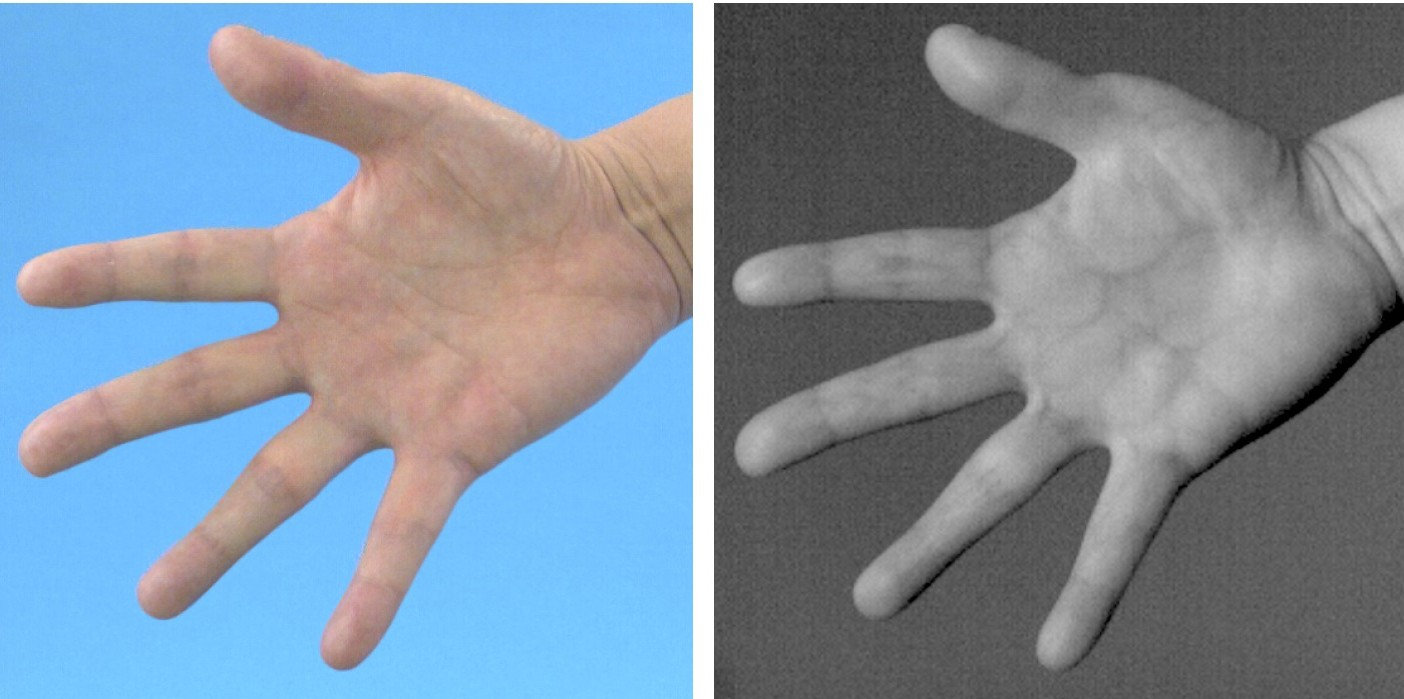
\includegraphics[width=0.8\textwidth]{imgs/nir-hand.jpg}
    \caption{Left image is RGB, right image is NIR. Figure reproduced from~\cite{Monno2019RGBNIR}.}
    \label{fig:hand_nir}
\end{figure}

Remote sensing and environmental monitoring is another major use. Vegetation reflects NIR strongly because of its spongy mesophyll structure, which supports robust assessment of plant health, biomass, crop yield and drought~\cite{tucker1979red}. Unlike RGB, which is sensitive to illumination and surface colour, NIR gives a more stable measure of vegetation health.

NIR is also common in surveillance, night vision and autonomous driving. With active infrared illumination it images in low light and at night, where RGB cameras fail, and its longer wavelengths scatter less, which helps perception in fog or haze~\cite{he2011single}. In industrial inspection it supports material sorting, quality control and defect detection, since materials differ in NIR reflectance.

\section{Spectral Characteristics and Physics of NIR}
\label{sec:nir_physics}

NIR sits just beyond visible red, but what makes it useful is how it interacts with matter. Visible-light imaging mostly sees surface reflectance from pigments and dyes. NIR reflectance instead depends on molecular vibrations, water content and a material's internal structure~\cite{curran1989remote}. Because NIR also scatters and is absorbed less in organic matter, it penetrates further into skin, leaves and other semi-translucent subjects, picking up subsurface detail that visible light never reaches.

Materials that look distinct in RGB can look identical in NIR, and the reverse also happens. Healthy vegetation is green in RGB, because chlorophyll absorbs red and blue, but very bright in NIR, since chlorophyll does not absorb NIR (\autoref{fig:leaf_nir}). Water absorbs NIR strongly and appears dark, which makes NIR effective for water-body delineation and moisture analysis~\cite{gao1996ndwi}.

\begin{figure}[!htbp]
    \centering
    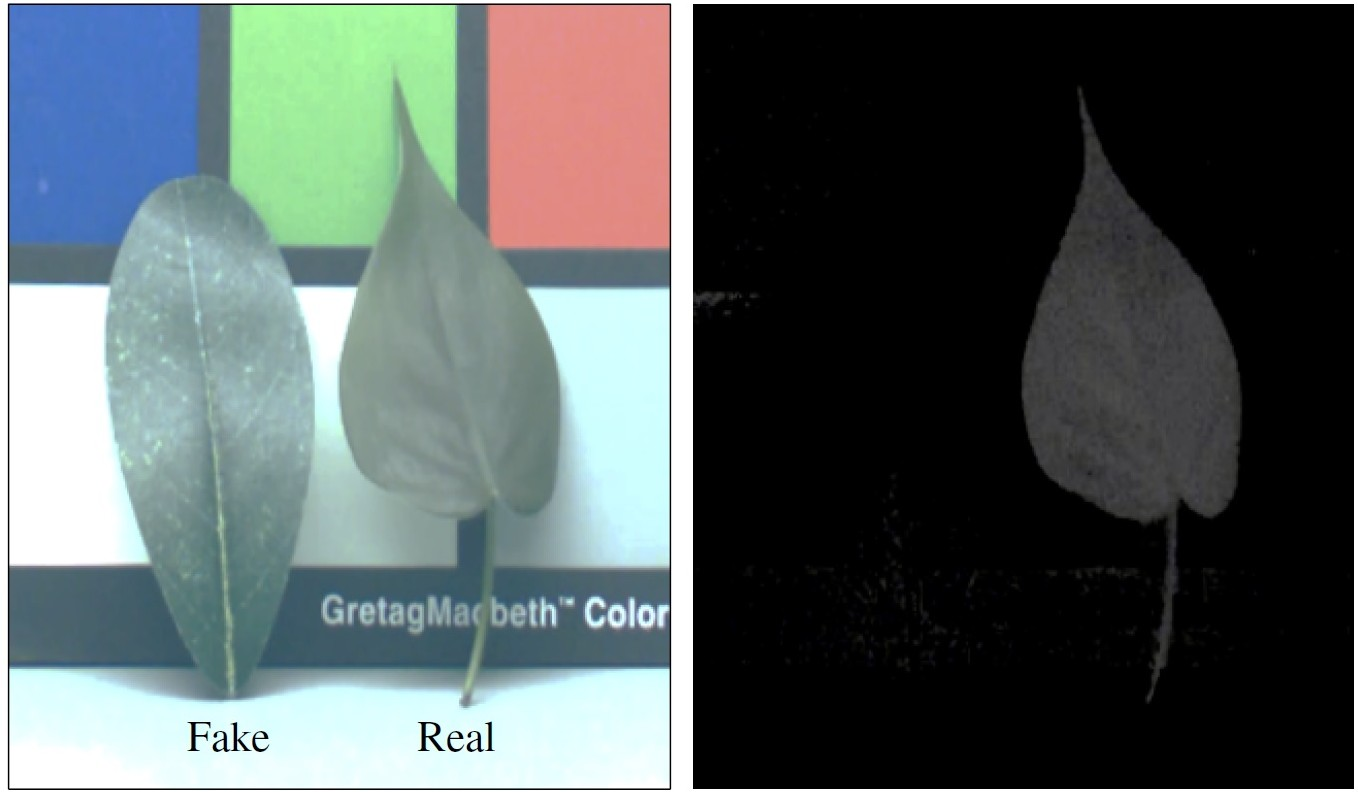
\includegraphics[width=0.8\textwidth]{imgs/leaf-nir.jpg}
    \caption{Left image is RGB, right image is NIR. Figure reproduced from~\cite{Monno2019RGBNIR}.}
    \label{fig:leaf_nir}
\end{figure}

\section{Visual and Textural Differences: NIR vs.\ RGB}
\label{sec:nir_rgb_differences}

The two bands diverge most in texture. In RGB, texture comes from colour gradients, shading and surface pigmentation. In NIR it comes from material composition, moisture and internal structure, which pushes edges, contrast and spatial-frequency content away from anything an RGB-trained model expects~\cite{salamati2010material,salamati2014incorporating}.

For example, skin looks uniform in RGB, its texture set by pores, wrinkles and pigmentation, but smoother in NIR, where subsurface veins become prominent (\autoref{fig:hand_nir}). Facial hair, prominent in RGB, is darker and less distinct in NIR, and fabrics with different RGB colours can look identical in NIR when the material is the same.

NIR is also less affected by shadows and specular highlights, giving smoother gradients and different edge responses. Convolutional filters and descriptors trained on RGB therefore behave differently on NIR. This mismatch in texture, contrast and spatial statistics is the core difficulty in cross-spectral understanding that NIR-to-RGB translation sets out to address.

\section{Impact on Machine Learning Performance}
\label{sec:nir_ml_impact}

These spectral and textural differences degrade machine-learning models trained only on RGB. Deep networks implicitly learn RGB statistics such as colour distributions, channel correlations and texture~\cite{krizhevsky2012imagenet}, and on NIR input those learned features often fail to fire because the input assumptions are violated. \autoref{fig:yolo_nir_rgb} compares the Ultralytics YOLOv8 Nano detector~\cite{jocher2023yolov8} on NIR and RGB.

\begin{figure}[!htbp]
    \centering
    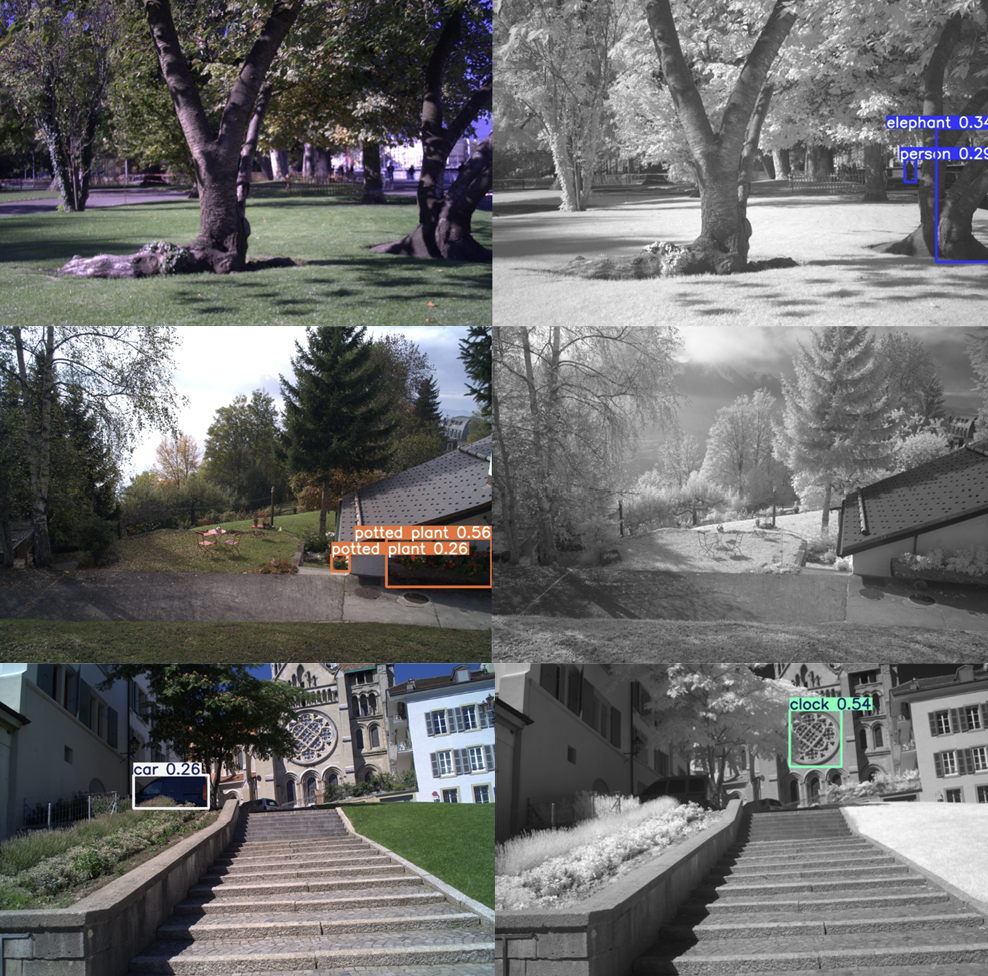
\includegraphics[width=0.8\textwidth]{imgs/poor.png}
    \caption{Ultralytics YOLOv8 Nano detector run on an RGB image (left) and the matching NIR image (right). NIR/RGB images from the EPFL RGB-NIR Scene Dataset~\cite{epfl_rgbnir_dataset}.}
    \label{fig:yolo_nir_rgb}
\end{figure}

Segmentation, detection and face-recognition models lean on colour and visible texture to separate classes. NIR lacks colour and has different intensity statistics, so early filters tuned for RGB edges and colour give weak or misleading activations~\cite{peng2018rgbnir,salamati2014incorporating}, and the models generalise poorly even when the semantic content is unchanged. \autoref{fig:nir_rgb_comparison} shows a segmentation model failing on a simple NIR case.

\begin{figure}[!htbp]
    \centering
    \begin{minipage}{0.39\textwidth}
        \centering
        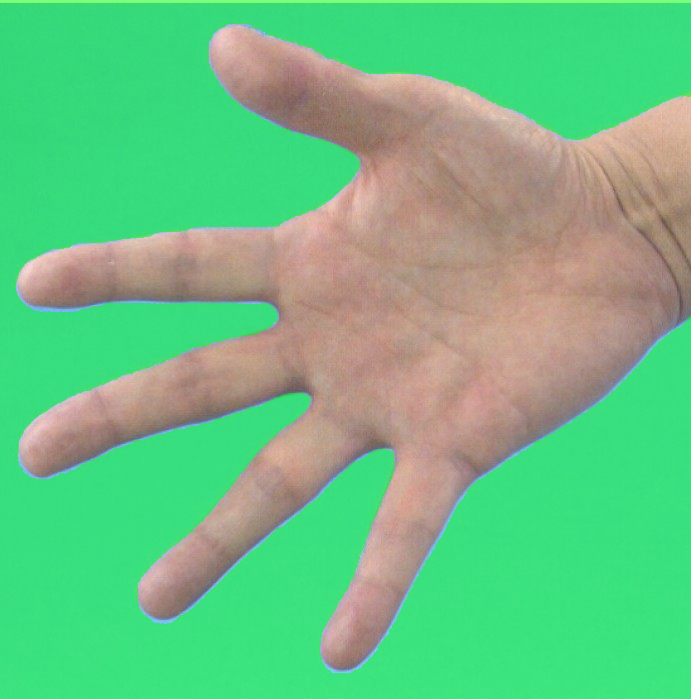
\includegraphics[width=\linewidth]{imgs/nir-hand2_mediapipe_overlay.png}
        \subcap{(a) RGB image}
    \end{minipage}
    \hspace{0.002\textwidth}
    \begin{minipage}{0.39\textwidth}
        \centering
        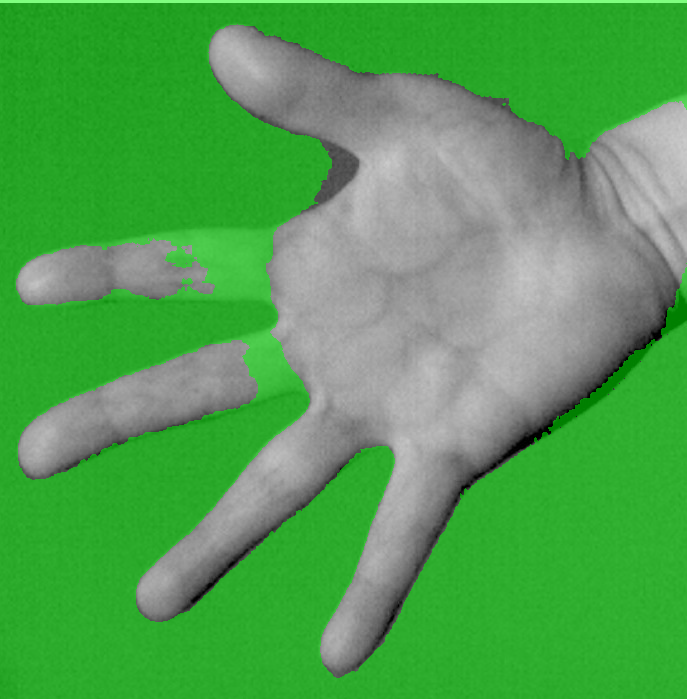
\includegraphics[width=\linewidth]{imgs/nir-hand1_mediapipe_overlay.png}
        \subcap{(b) NIR image}
    \end{minipage}
    \caption{Background (green overlay) segmentation from the MediaPipe Selfie Segmentation model~\cite{lugaresi2019mediapipe}. The same model fails to find a foreground subject on the NIR input.}
    \label{fig:nir_rgb_comparison}
\end{figure}

Although the NIR camera records a three-channel image, all three channels sample the same band beyond the 850\,nm filter, so they are highly correlated and carry no colour information: the input is spectrally single-band even though it is stored as three channels. This removes the cross-channel structure that RGB models rely on for robustness. Translating NIR to RGB is therefore a practical adaptation strategy: it produces RGB-like images that better match the feature space of pretrained RGB models~\cite{isola2017image}.

While the examples above use single detectors, the degradation is systematic across architectures rather than an artefact of one model. To confirm this on the data collected for this project (Chapter~\ref{ch:implementation}), a panel of nine modern semantic-segmentation transformers was run on paired NIR and RGB frames. The panel covers SegFormer~\cite{xie2021segformer}, BEiT~\cite{bao2022beit} and Mask2Former~\cite{cheng2022mask2former} variants trained on the ADE20K~\cite{zhou2017ade20k} and Cityscapes~\cite{cordts2016cityscapes} benchmarks, and for each model the agreement between its NIR and RGB segmentations was measured per object category. The loss of agreement is substantial but non-uniform. Vegetation and person regions, whose NIR appearance departs most from the visible band, degrade far more than road or building surfaces, and the smaller, more deployable models degrade more than the larger ones. This last point is particularly important in an edge setting, since the efficient models most likely to be deployed are also the most fragile on NIR input. This motivates placing a lightweight NIR$\rightarrow$RGB translator ahead of them. The downstream evaluation of Chapter~\ref{ch:results} measures how much of that agreement the translator developed here restores for the panel's most deployable architecture, SegFormer-B0, on both its ADE20K and Cityscapes variants (Section~\ref{sec:res_seg}).

Figures~\ref{fig:seg_fail_mask2former} and \ref{fig:seg_fail_beit} make these failure modes concrete for two of the panel's architectures. In each, the top row shows the RGB and raw-NIR inputs and the bottom row the corresponding segmentations. The overlay colours are green for vegetation, yellow for buildings, red for people and blue for road, and the per-category Dice agreement with the RGB segmentation is printed on each example. They show that the collapse is selective. Classes whose NIR appearance departs most from the visible band fail, while structurally similar surfaces such as road are often preserved.

\begin{figure}[!htbp]
    \centering
    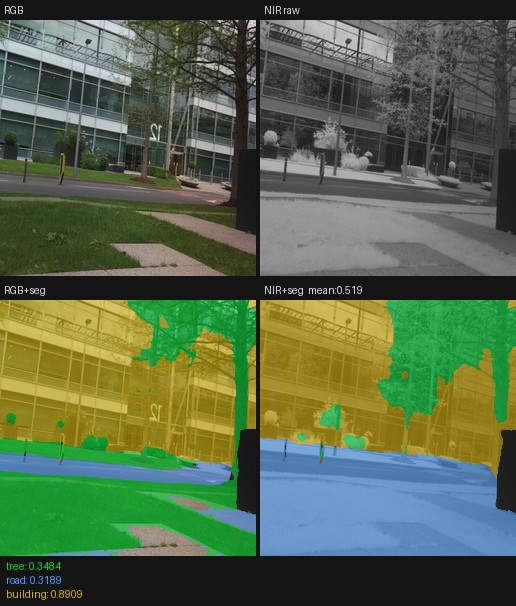
\includegraphics[width=0.78\textwidth]{imgs/mask2former-fail.jpg}
    \caption{Mask2Former (ADE20K) Overlay key: green = vegetation, yellow = building, red = person, blue = road. The building is largely recovered on NIR (Dice 0.89), but the bright NIR foliage and pavement are misread: vegetation collapses to 0.35 and the path is misclassified as road (0.32).}
    \label{fig:seg_fail_mask2former}
\end{figure}



\begin{figure}[!htbp]
    \centering
    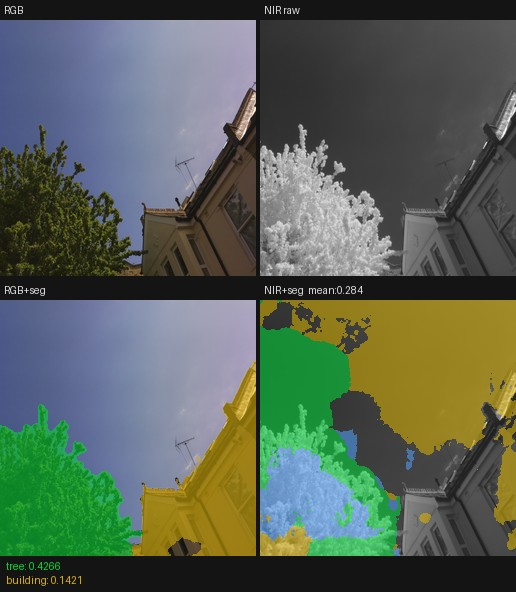
\includegraphics[width=0.78\textwidth]{imgs/beit-fail.jpg}
    \caption{BEiT (ADE20K) on a building and tree scene against sky (mean Dice 0.28)}
    \label{fig:seg_fail_beit}
\end{figure}

\section{Image-to-Image Conversion}
\label{sec:i2i_overview}

Image-to-image conversion learns a mapping between two visual representations of the same content. Modern methods are data-driven, learning non-linear mappings from paired or unpaired data rather than using hand-crafted transforms. For NIR-to-RGB the goal is to turn near-infrared images into plausible RGB while preserving semantic and structural content. This is hard because the NIR input has no colour, so many RGB appearances fit the same NIR observation~\cite{gonzalez2002digital}.

The same problem can be framed as domain adaptation: the translator maps a source distribution $P_{\text{NIR}}$ onto a target distribution $P_{\text{RGB}}$, so that models trained on $P_{\text{RGB}}$ continue to work on inputs originally drawn from $P_{\text{NIR}}$ without retraining~\cite{bendavid2010theory}. This connects NIR-to-RGB translation to the wider literature on covariate shift and feature alignment, and to image-translation-based adaptation methods such as CyCADA~\cite{hoffman2018cycada}, which use a learned image translator as the adaptation mechanism rather than retraining the downstream model. The approach taken in this project follows that pattern: instead of fine-tuning the frozen RGB-pretrained models for NIR input, the input distribution is mapped toward the one those models were trained on.

\subsection{Pre-Deep Learning Approaches}
\label{sec:i2i_classical}

Before deep learning, cross-spectral conversion relied on classical signal processing: linear or piecewise-linear intensity mappings, histogram equalisation and specification to align global statistics, and patch-based methods that matched source patches against a target-domain dictionary~\cite{efros1999texture}. These techniques are computationally cheap, but they either ignore spatial context entirely or depend on handcrafted features that break down under large scene variation. They lack the capacity to model the non-linear, context-sensitive NIR-to-RGB relationship, which motivated the shift to learning-based methods.

\subsection{Deep Learning for Image-to-Image Conversion}
\label{sec:i2i_dl}

Deep learning enabled end-to-end conversion with convolutional neural networks (CNNs). Early models used encoder--decoder architectures: the encoder compresses the input to a latent representation and the decoder reconstructs the target-domain image. These learn spatially varying transforms and capture semantic context, which suits cross-spectral conversion~\cite{dong2015image}.

Fully convolutional networks with skip connections, such as U-Net~\cite{ronneberger2015unet}, were a key step. Skip connections pass low-level spatial detail from early layers straight to later ones, preserving fine detail and sharp edges. That matters for NIR-to-RGB, where structure must be kept while colour is synthesised.

Pixel losses (L1 or L2) enforce fidelity to the ground-truth RGB but blur outputs, since they average over plausible solutions. Perceptual losses address this limitation by comparing high-level features from pretrained networks rather than raw pixels, giving sharper, more semantically meaningful results~\cite{johnson2016perceptual}.

\subsection{Generative Adversarial Networks}
\label{sec:i2i_gan}

A generative adversarial network (GAN) trains a generator against a discriminator so the output matches the target domain's statistics, not just its mean pixel values~\cite{goodfellow2014generative}. The paired variant, the conditional GAN, adds a reconstruction term that ties the output back to the input~\cite{isola2017image}. For aligned NIR/RGB captures this provides a natural baseline: the reconstruction term constrains structure while the adversarial term encourages target-domain appearance.

Pix2pix is the standard cGAN for paired translation: a U-Net generator for spatial detail, a PatchGAN discriminator for local realism, and an L1 reconstruction term~\cite{isola2017image}. Since its introduction it has become the de facto baseline for paired image-to-image translation, and the dominant methods that followed are direct descendants of it, including the high-resolution Pix2pixHD~\cite{wang2018pix2pixhd}, semantic-conditioned SPADE~\cite{park2019spade}, and, in the cross-spectral setting closest to this work, Pix2Next~\cite{pix2next2024}. It is also applied directly to cross-spectral RGB/NIR translation, for example mapping RGB to NIR for fire detection~\cite{akagic2023rgbnir}. It was used as the baseline here because it is straightforward to train and export, and because it is the established formulation any more complex method should be expected to improve on.

\subsection{Limitations of pix2pix for NIR-to-RGB}
\label{sec:pix2pix_limitations}

Three limitations of pix2pix are particularly important in the cross-spectral setting. First, it assumes well-aligned pairs. Even a few pixels of NIR/RGB misregistration can be learned as colour ``halos'' or edge ghosting, while precise pairs are difficult to collect (Section~\ref{sec:datasets}). Second, the mapping is one-to-many because colour is not directly present in the NIR input. An L1-trained deterministic generator can therefore converge toward dataset-average colours and mis-colour materials that share similar NIR responses. Third, the PatchGAN objective rewards local realism, which can produce globally inconsistent texture, subtle tiling or over-sharpening that appears acceptable in small crops but less coherent in full frames. These limitations do not prevent pix2pix from serving as a baseline, but they identify the main areas in which a better translator must improve.

\subsection{Pix2pixHD: high-resolution conditional GANs}
\label{sec:pix2pixhd}

Pix2pixHD scales pix2pix to high resolution~\cite{wang2018pix2pixhd}. Two of its ideas remain especially relevant: a coarse-to-fine generator that establishes global layout before adding fine detail, and multi-scale discriminators that evaluate coarse structure and local texture separately rather than at one fixed patch size. It also adds a feature-matching loss on discriminator activations, which stabilises training and discourages the generator from satisfying the PatchGAN through high-frequency artefacts at the expense of semantic consistency. This feature-matching idea is important for the present project, where matching intermediate representations becomes a way to preserve structure while adapting appearance (Chapter~\ref{ch:design}).

\subsection{Pix2Next: Vision foundation models for RGB$\rightarrow$NIR translation}
\label{sec:pix2next}

Pix2Next is the closest prior work to this project, even though it runs in the opposite direction, RGB$\rightarrow$NIR~\cite{pix2next2024}. It incorporates a frozen pretrained vision model into a Pix2pixHD-style backbone and injects those global features into the generator through cross-attention, so the colour synthesised at a pixel can draw on the whole scene rather than a local patch. Training adds SSIM and feature-matching terms to the adversarial loss to preserve structure.

Two aspects of Pix2Next shaped the approach taken here. First, global features from a large pretrained model provide a practical way to maintain scene-level coherence when paired data are limited. Second, Pix2Next evaluates not only image similarity but also whether the generated output improves a downstream detector. This project adopts the same principle for the reverse NIR$\rightarrow$RGB direction: evaluation is centred on downstream model behaviour rather than image-quality scores alone (Chapter~\ref{ch:design}). Across this line of work, from the perceptual loss~\cite{johnson2016perceptual} through Pix2pixHD's feature matching to Pix2Next's pretrained conditioning and SPADE-style semantic conditioning~\cite{park2019spade}, the common thread is to keep a pretrained network's intermediate activations similar before and after translation, which is the idea the design of this project builds on (Chapter~\ref{ch:design}).

\subsection{Diffusion and Bridge Models for Image-to-Image Conversion}
\label{sec:i2i_diffusion}

Diffusion models generate by iterative denoising: noise is added gradually and the reverse process learns to remove it~\cite{ho2020denoising}. Conditioned on an input such as NIR, they capture the one-to-many ambiguity of colour and produce high-quality, diverse samples, and they train more stably than GANs~\cite{saharia2022image}. In principle, this is well suited to NIR$\rightarrow$RGB, where one NIR frame admits several plausible colourings. Bridge models, including Schr\"odinger bridges, extend the same idea by learning a stochastic transport between two distributions under fixed endpoints, and recent methods are competitive on translation tasks~\cite{leonard2013survey,debortoli2021neural}. Both families, however, share two properties that conflict with this project's deployment target: inference is iterative, requiring many network passes per image, and it is stochastic. Why these properties rule them out here is set out in Section~\ref{sec:why_not_diffusion}.

\subsection{Efficient Restoration Networks for Edge Translation}
\label{sec:i2i_nafnet}

The generative families above (conditional GANs, diffusion and bridge models) prioritise sample realism and the ability to represent one-to-many ambiguity, but they incur either adversarial instability or many denoising steps per image. This cost is difficult to reconcile with a translator that must run deterministically within a small per-frame budget on an edge device. A separate line of work, image restoration, offers an alternative: efficient feed-forward CNNs that map a degraded image to a clean one in a single pass. NAFNet (Nonlinear Activation-Free Network)~\cite{chen2022nafnet} is a prominent example. It reaches state-of-the-art results on denoising and deblurring while stripping the architecture back to a minimal operator set, replacing every nonlinear activation with a multiplicative ``SimpleGate''. That minimal, predictable operator set makes it attractive for constrained hardware, since it exports cleanly to embedded inference runtimes and behaves well under low-bit quantisation.

Restoration networks are usually designed for same-modality problems, where input and output show the same scene under the same imaging conditions (for example noisy$\rightarrow$clean). In that setting the network primarily removes a degradation rather than inferring missing spectral information. NIR$\rightarrow$RGB is harder: colour absent from the input must be inferred from material, texture and scene context. For this reason, using a restoration backbone for cross-spectral translation is a non-standard choice. Prior NIR$\rightarrow$RGB work has more often used generative architectures such as cycle-consistent or conditional GANs, and more recently diffusion models (Sections~\ref{sec:i2i_gan}--\ref{sec:i2i_diffusion}). The literature reviewed for this report did not identify previous use of NAFNet for NIR$\rightarrow$RGB translation. Its strong feed-forward capacity and quantisation-friendly, activation-free design make it a strong candidate for an edge-deployable translator.

\subsection{Availability of Paired RGB--NIR Datasets (and Practical Limitations)}
\label{sec:datasets}

Publicly available RGB--NIR paired datasets exist, but they are relatively small and often are not perfectly paired. A commonly used example is the RGB--NIR Scene Dataset released with Brown and S\"usstrunk's multispectral SIFT work~\cite{brown2011multispectral,epfl_rgbnir_dataset}. It contains aligned RGB and NIR images across several outdoor scene categories, but the RGB and NIR frames are captured using separate exposures with different filters (visible vs.\ NIR, with a cutoff around 750\,nm) and then registered using SIFT~+~RANSAC~\cite{epfl_rgbnir_dataset}. While this produces useful approximate alignment, any motion between NIR and RGB captures (cars, pedestrians, foliage, water) leads to non-matching content. \autoref{fig:epfl_rgbnir_dataset} shows an example of this. Content differences of this kind make such data unsuitable as supervised training pairs for NIR$\rightarrow$RGB translation, because the network would be penalised for failing to reproduce people and objects that are not in the same place in the target frame. This limitation directly motivates the bespoke capture rig built for this project, which images both bands through a shared aperture so that every pair is simultaneous and related by a single depth-independent homography (Chapter~\ref{ch:implementation}).

\begin{figure}[!htbp]
    \centering
    \begin{minipage}[b]{0.42\textwidth}
        \centering
        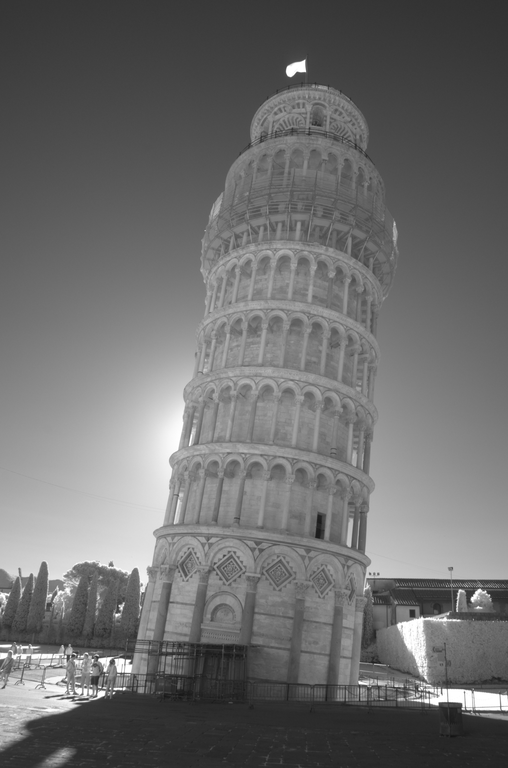
\includegraphics[width=\linewidth]{imgs/0001_nir.png}
        \subcap{(a) NIR image}
    \end{minipage}\hfill
    \begin{minipage}[b]{0.42\textwidth}
        \centering
        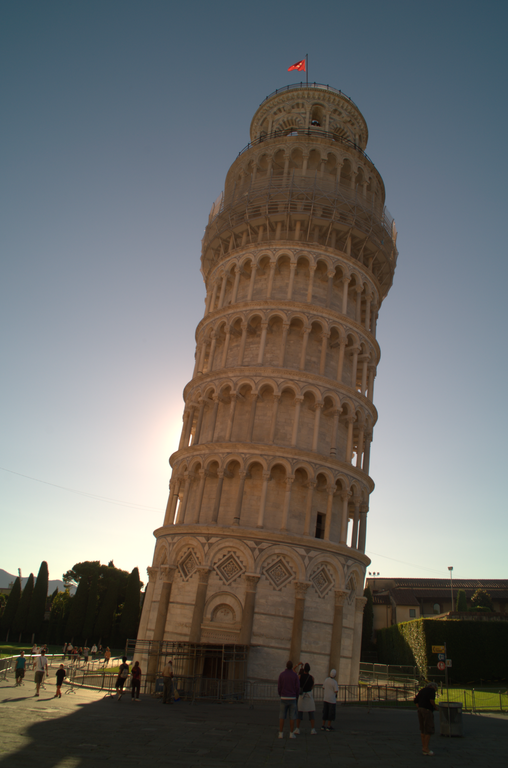
\includegraphics[width=\linewidth]{imgs/0001_rgb.png}
        \subcap{(b) RGB image}
    \end{minipage}
    \caption{An imperfectly paired sample from the EPFL RGB--NIR Scene Dataset~\cite{epfl_rgbnir_dataset,brown2011multispectral}. The tower aligns across bands, but the pedestrians in the foreground have moved between the two exposures. This is a content mismatch that post-hoc registration cannot correct.}
    \label{fig:epfl_rgbnir_dataset}
\end{figure}

\section{Model Compression for Edge Deployment}
\label{sec:model_compression}

A translator that reaches high image quality is usually too large to run inside a per-frame budget on an edge device. The gap between a strong model and a deployable one is normally closed with two complementary techniques: knowledge distillation, which trains a small network to behave like a large one, and quantisation, which stores and computes that network at lower numerical precision. Both are used in this project, so the underlying ideas are summarised here before the design and implementation chapters apply them.

\subsection{Knowledge Distillation}
\label{sec:kd}

Knowledge distillation trains a compact student network to reproduce the behaviour of a larger teacher rather than learning the task from labels alone~\cite{hinton2015distilling}. The original formulation matches the teacher's softened output distribution, on the argument that the teacher's full response carries more information than a hard target. Later work showed that the student can also be supervised on the teacher's intermediate activations, so that it imitates how the teacher represents an input and not only what it predicts~\cite{romero2015fitnets}.

For image translation the same idea applies at the level of pixels and features. The student is trained to reproduce the teacher's output image, optionally with a small anchor to the ground truth, and can additionally be asked to match feature representations extracted from frozen networks. This is the route taken for the edge model in this project, where a width-16 student is distilled from the width-64 teacher (Chapter~\ref{ch:implementation}).

\subsection{Quantisation}
\label{sec:quantisation}

Quantisation represents weights and activations with lower-precision integers, typically 8-bit (INT8) instead of 32-bit floating point. This shrinks the model and, more importantly on a CPU, lets inference use faster integer kernels~\cite{jacob2018quantization,gholami2021survey}. The two common regimes differ in when quantisation is introduced. Post-training quantisation (PTQ) converts an already-trained model, calibrating the integer ranges from a small set of representative images and requiring no further training. Quantisation-aware training (QAT) instead simulates the rounding during training so the network can adapt to it, which usually recovers more accuracy~\cite{jacob2018quantization}.

This work uses PTQ. The activation-free design of the chosen backbone (Section~\ref{sec:i2i_nafnet}) provides a compact operator set for mixed-INT8 export, although unsupported LayerNorm and PixelShuffle-adjacent operations remain in FP32. The implementation compares static and Q/DQ export paths, and Chapter~\ref{ch:results} reports off-device numerical equivalence and quality retention. On-device latency and memory are measured on the Raspberry~Pi~5 in Section~\ref{sec:res_edge}.
 % Background
\doublespacing % Do not change - required

\chapter{Requirements and Design}
\label{ch:requirements}
\label{ch:design}

%%%%%%%%%%%%%%%%%%%%%%%%%%%%%%%%%%%%%%%
% IMPORTANT
\begin{spacing}{1} %THESE FOUR
\minitoc % LINES MUST APPEAR IN
\end{spacing} % EVERY
\thesisspacing % CHAPTER
% COPY THEM IN ANY NEW CHAPTER
%%%%%%%%%%%%%%%%%%%%%%%%%%%%%%%%%%%%%%%

This chapter turns the motivation of Chapter~\ref{ch:introduction} into a specification and then into a design. It sets out who the deliverable is for, what it must do and the constraints it must respect, and then explains the architecture, loss and evaluation choices that follow from those requirements. The as-built configuration and the measured numbers are given in Chapter~\ref{ch:implementation}, and the requirements defined here are revisited in the critical evaluation of Chapter~\ref{ch:evaluation}.

\section{Intended Use}
\label{sec:req_stakeholders}

The deliverable is a NIR$\rightarrow$RGB pre-processor, a module placed between a near-infrared sensor and an existing RGB-trained vision model. Its user is an engineer who already has a working RGB perception stack, such as an object detector, a segmentation network or a depth model, and a reason to run it on NIR input such as night operation, biometric imaging or material inspection.

The direct alternative is to retrain or fine-tune each downstream model on NIR data, but this is often impractical. It needs the model weights to be openly available, and it needs a large amount of NIR data to be collected and labelled for every task. A single translator that restores RGB-like performance avoids most of this cost and leaves each downstream model unchanged.

\section{Functional Requirements}
\label{sec:req_functional}

\begin{enumerate}
    \item \textbf{F1: Translation.} Map a 3-channel NIR image to a 3-channel RGB image of the same scene at the same resolution.
    \item \textbf{F2: Geometry preservation.} Preserve spatial structure. Object boundaries, thin structures and positions must not move, so that a downstream model's spatial outputs remain valid.
    \item \textbf{F3: Determinism.} Produce the same output for the same input. As a stage in a perception pipeline, stochastic output would inject noise into every downstream model.
    \item \textbf{F4: Drop-in interface.} Accept the sensor's native frames and produce standard 8-bit RGB, so the downstream model is used unmodified.
\end{enumerate}

\section{Non-Functional Requirements}
\label{sec:req_nonfunctional}

\begin{enumerate}
    \item \textbf{N1: Throughput.} Run at an interactive frame rate of around 5\,FPS, roughly 200\,ms per frame, at the deployment resolution on the target Raspberry~Pi~5 CPU.
    \item \textbf{N2: Edge footprint.} Fit within the compute and memory budget of the target device after INT8 quantisation. The deployed model must load and run without swapping or an out-of-memory failure while meeting N1. Artefact size and peak resident memory are reported for the distilled student of Section~\ref{sec:edge_student}.
    \item \textbf{N3: Quality measured by downstream utility.} Judge success by how much downstream-task performance is recovered relative to native RGB, the gap-closure metric of Section~\ref{sec:design_evaluation}, rather than by pixel fidelity such as PSNR alone.
\end{enumerate}


\section{Design Goals}
\label{sec:design_goals}

The requirements lead to four design drivers, which together point to a single class of solution.

\begin{itemize}
    \item \textbf{Semantic preservation over photorealism.} The output is consumed by frozen RGB-pretrained models, not by human viewers, so edges, boundaries, thin structures and material identity matter more than absolute colour accuracy. This follows from F2 and N3.
    \item \textbf{Deterministic, low-latency inference.} The translator must give the same output for the same input and run in a small, predictable per-frame budget. This follows from F3 and N1.
    \item \textbf{Edge deployment on the Raspberry~Pi~5.} This rules out architectures whose operators are unsupported by the chosen Pi~5 runtime, and any whose compute or memory footprint exceeds what the device can sustain in real time. This follows from N1 and N2.
    \item \textbf{Paired supervision from a small bespoke dataset.} Public RGB--NIR pairs are limited and often imperfectly aligned, as discussed in Section~\ref{sec:datasets}, so a dedicated capture rig is required.
\end{itemize}

Together these favour a deterministic, supervised feed-forward translator with strong structural regularisation. This excludes both an unpaired CycleGAN-style approach and a stochastic diffusion model. The rest of the chapter works through the architecture, loss and evaluation choices that follow.

\section{Semantic Preservation and ``Semantic Drift''}
\label{sec:semantic_drift}

Image-to-image translation can lose semantics during conversion. Even a photorealistic output may move object boundaries, drop small but meaningful structures, or hallucinate edges and textures that were not in the input. NIR-to-RGB is especially exposed to this because the model must also infer colour. Where the training data correlates particular materials or backgrounds with particular colours, the generator can over-rely on those priors and alter the scene in semantically important ways.

This semantic drift matters most when translated images feed downstream tasks such as detection, segmentation and identity recognition, where small geometric warps, boundary shifts or spurious high-frequency detail hurt performance more than colour errors do. The standard mitigations are reviewed in Sections~\ref{sec:pix2pixhd} and~\ref{sec:pix2next}. The decision taken here is to push that idea further and supervise on the deep features the downstream models actually use, as set out in the loss design of Section~\ref{sec:loss_design}.  \autoref{fig:pix2pix_semantic_drift} shows it observed directly in an early experiment for this project, in which a pix2pix model trained on the KAIST thermal benchmark fails to preserve a roadside sign that is clearly visible in the input.

\begin{figure}[!htbp]
    \centering
    \begin{minipage}{0.31\textwidth}
        \centering
        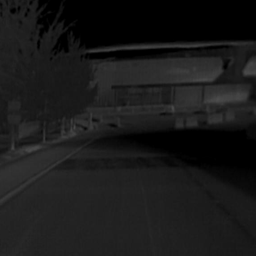
\includegraphics[width=\linewidth]{imgs/pix2pix-poor-semantic-result/IR-image.png}
        \subcap{(a) LWIR input}
    \end{minipage}\hfill%
    \begin{minipage}{0.31\textwidth}
        \centering
        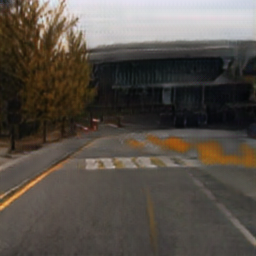
\includegraphics[width=\linewidth]{imgs/pix2pix-poor-semantic-result/RGB-fake.png}
        \subcap{(b) pix2pix output}
    \end{minipage}\hfill%
    \begin{minipage}{0.31\textwidth}
        \centering
        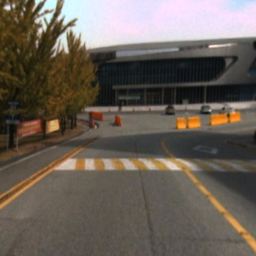
\includegraphics[width=\linewidth]{imgs/pix2pix-poor-semantic-result/RGB-real.png}
        \subcap{(c) Ground-truth RGB}
    \end{minipage}
    \caption{Example of semantic drift in long-wave infrared (LWIR)$\rightarrow$RGB translation, produced by a pix2pix model trained for this project on the KAIST RGB--thermal benchmark~\cite{hwang2015multispectral}}
    \label{fig:pix2pix_semantic_drift}
\end{figure}

\section{Architecture Choice}
\label{sec:architecture_choice}

Two architecture families were considered.

\begin{description}
    \item[Pix2Pix U-Net (baseline).] A Pix2Pix-style 8-level U-Net generator with a PatchGAN discriminator is the canonical paired-translation baseline~\cite{isola2017image} and the formulation most later paired-translation methods build on, which makes it a strong and fair point of comparison. Its strengths are sharp output, simple training and easy export, and its weaknesses are well documented: it is BatchNorm-heavy, has around 54\,M parameters at base width 64, and is prone to semantic drift under one-to-many ambiguity.
    \item[NAFNet teacher (selected).] NAFNet~\cite{chen2022nafnet} is a modern simple-baselines architecture for image restoration. Compared to the Pix2Pix U-Net it has no nonlinear activations, using a SimpleGate and channel attention instead, which gives stable training and predictable INT8 quantisation. Its layer-normalised blocks behave well at small batch sizes, and its pure-CNN structure exports cleanly to ONNX and the common Pi~5 runtimes such as ONNX Runtime, NCNN and TFLite. The teacher uses the width-64 configuration, with $[2,2,4,8]$ encoder blocks and 12 middle blocks, for around 116\,M parameters. The as-built model is detailed in Section~\ref{sec:nafnet_teacher}.
\end{description}

\subsection{Edge Student}
\label{sec:edge_student}

The NAFNet teacher is large because it is not the deployed model. A smaller width-16 NAFNet, with reduced width and block depth, is distilled from it and quantised to INT8 for the Raspberry~Pi~5 CPU, as described in Section~\ref{sec:edge_deployment}. Separating teacher from student lets the teacher train at full quality on a desktop GPU while the student is shaped to the latency and memory budget of the deployment target.

\section{Loss Design}
\label{sec:loss_design}

The starting point is the standard objective for paired image translation: an L1 reconstruction term for colour fidelity, a VGG-16 perceptual term for feature-space similarity~\cite{johnson2016perceptual}, a least-squares PatchGAN term for local realism, and a multi-scale SSIM term for structural fidelity~\cite{wang2003msssim}.

The central design decision of this project is to change what the perceptual supervision matches. Because the translated image is consumed by frozen RGB-pretrained networks rather than by a human, the objective that best serves the goal is agreement in the deep-feature spaces those networks use, which is the quantity the downstream evaluation measures in Section~\ref{sec:design_evaluation}. A single ImageNet-VGG perceptual term captures only one such space. The final teacher therefore replaces it with a set of frozen foundation models: DINOv2~\cite{oquab2024dinov2} for self-supervised features, CLIP~\cite{radford2021clip} for vision--language features, and ResNet-50~\cite{he2016resnet} for ImageNet-supervised features. Matching features across this ensemble pushes the output to sit within the input distribution of many representations rather than one, as a task-agnostic pre-processor requires.

Formally, writing $T$ for the translator and $F$ for a frozen feature extractor, training pushes $F(T(x_{\text{NIR}})) \approx F(x_{\text{RGB}})$ for each $F$ in the ensemble, so a downstream model whose predictions depend on $F(\cdot)$ behaves on $T(x_{\text{NIR}})$ more like it does on $x_{\text{RGB}}$. The gap-closure metric of Section~\ref{sec:design_evaluation} measures empirically how well this holds for each downstream task.

The final recipe keeps the stabilising parts of the conventional objective: a strong L1 colour anchor, an MS-SSIM structural term and a lightly weighted PatchGAN term. The VGG perceptual term is dropped, since it captures only one ImageNet feature space, and the foundation ensemble supplies the task-facing perceptual signal in its place. The exact weights are given in Section~\ref{sec:nafnet_teacher} and \autoref{tab:teacher_loss}.

\section{Why Not Diffusion or Bridge Models?}
\label{sec:why_not_diffusion}

Conditional diffusion and bridge models (Section~\ref{sec:i2i_diffusion}) represent the one-to-many ambiguity of NIR$\rightarrow$RGB colourisation well, but they were rejected on two grounds. Sampling requires many denoising steps, which is incompatible with the 200\,ms-per-frame target on the Raspberry~Pi~5, where a single forward pass through a NAFNet student is comparable in cost to one diffusion step. And their sampling is stochastic, which violates the determinism requirement F3 by construction. Schr\"odinger-bridge formulations remain interesting for offline data augmentation, for example synthesising additional NIR/RGB pairs from one-sided data, but not for deployment.

\section{Evaluation Design}
\label{sec:design_evaluation}

Standard image-quality metrics such as PSNR, SSIM and LPIPS measure how close the translated RGB is to ground-truth RGB. They do not measure whether downstream pretrained models work better on the translated image, which is this project's goal. To address this, a downstream evaluation harness was designed. It runs a panel of frozen RGB-pretrained networks on three inputs, raw NIR, translated RGB and ground-truth RGB, and reports a per-task \emph{gap closure}
\[
\text{gap\_closure} \;=\; \frac{m(\text{translated}) - m(\text{nir})}{m(\text{rgb}) - m(\text{nir})}
\]
where $m(\cdot)$ is the primary metric of the downstream task, for example matched detection Intersection over Union (IoU) or semantic-segmentation mean IoU (mIoU). A value of 0 means the translation is no better than raw NIR, 1 means native-RGB behaviour is fully recovered and a negative value means the translation made the task worse than raw NIR. For metrics where lower is better, such as the per-image normalised depth error used in Chapter~\ref{ch:results}, $m(\cdot)$ is defined so that the sign convention above still holds, with the harness inverting the raw difference accordingly. Full results are reported in Chapter~\ref{ch:results}.

\section{Success Criteria and Risk Register}
\label{sec:req_success}

The project is successful if it meets three criteria. S1, a paired and geometrically aligned NIR/RGB dataset is collected at sufficient scale for supervised training. S2, the translator yields positive gap closure on a majority of the downstream panel, at least three of the five tasks, with no task driven below its raw-NIR baseline. S3, the deployed student meets the 5\,FPS throughput target of N1 on the Pi~5. The quantitative thresholds and the final scoring against these criteria are reported in Chapters~\ref{ch:results} and~\ref{ch:evaluation}.

The main risks to these outcomes, and the design choices that mitigate them, are summarised in \autoref{tab:risk_register}.

\enlargethispage{3\baselineskip}
\begin{table}[!htbp]
\centering
\footnotesize
\begin{tabular}{p{0.30\linewidth}p{0.60\linewidth}}
\hline
\textbf{Risk} & \textbf{Mitigation} \\
\hline
Imperfectly aligned NIR/RGB pairs corrupt supervision (S1) & Shared-aperture capture rig, so each pair is simultaneous and related by a single depth-independent homography (Section~\ref{sec:datasets}). \\
Semantic drift toward dataset-average colour (S2) & Feature-space supervision against a foundation ensemble, with evaluation on downstream tasks rather than pixel fidelity (Sections~\ref{sec:loss_design} and~\ref{sec:design_evaluation}). \\
Student misses the latency budget on the Pi~5 (S3) & Width-16 distilled student, INT8 quantisation, and selection of the fastest supported runtime (Section~\ref{sec:edge_deployment}). \\
Limited paired data leads to overfitting (S1, S2) & Data augmentation and task-agnostic foundation-feature supervision rather than reliance on one feature space. \\
\hline
\end{tabular}
\caption{Principal project risks and the design choices that mitigate them.}
\label{tab:risk_register}
\end{table}
 % Requirements and Design (merged: was Requirements + Analysis and Design)
% % This chapter has been merged into Chapter3.tex ("Requirements and Design").
% The file is intentionally left unused and is no longer \input from main.tex.
% Kept as a placeholder so the chapter-numbering history is traceable.
 % merged into Chapter3.tex
\doublespacing % Do not change - required

\chapter{Implementation}
\label{ch:implementation}

%%%%%%%%%%%%%%%%%%%%%%%%%%%%%%%%%%%%%%%
% IMPORTANT
\begin{spacing}{1} %THESE FOUR
\minitoc % LINES MUST APPEAR IN
\end{spacing} % EVERY
\thesisspacing % CHAPTER
% COPY THEM IN ANY NEW CHAPTER
%%%%%%%%%%%%%%%%%%%%%%%%%%%%%%%%%%%%%%%

This chapter documents the system as built, in the order the data flows through it. Section~\ref{sec:data_collection_pi} describes the paired-capture rig and the data collection, Section~\ref{sec:alignment_pipeline} the pipeline intended to produce aligned training pairs, and Appendix~\ref{app:ethics} the ethical and privacy considerations. Section~\ref{sec:nafnet_teacher} then details the NAFNet teacher, its block structure, training objective and convergence, and Section~\ref{sec:edge_deployment} the distillation, export and quantisation that produce the deployment-target student. The design rationale behind these choices is given in Chapter~\ref{ch:design}, and the numbers they produce are reported in Chapter~\ref{ch:results}.

\section{Data Collection}
\label{sec:data_collection_pi}

Supervised NIR$\rightarrow$RGB translation requires a paired dataset in which each NIR frame corresponds, pixel for pixel, to a visible RGB frame of the same image. No public dataset met this requirement (Section~\ref{sec:datasets}), so a bespoke capture rig was built and used to collect a large, urban dataset of London's streets.

\subsection{Capture rig}
\label{sec:hardware_setup}

The rig is a self-contained unit housed in a 3D-printed case (Figure~\ref{fig:capture_rig}). It contains a Raspberry Pi~5 and two Raspberry Pi Camera Module~3 sensors: one captures the visible RGB image, the other captures NIR through an 850\,nm IR long-pass filter that blocks visible light. To give both cameras the same optical perspective incoming light passes through a beam-splitter cube that divides it between the two sensors, so both image the scene through a shared aperture.

\begin{figure}[!htbp]
    \centering
    \begin{minipage}{0.62\textwidth}
        \centering
        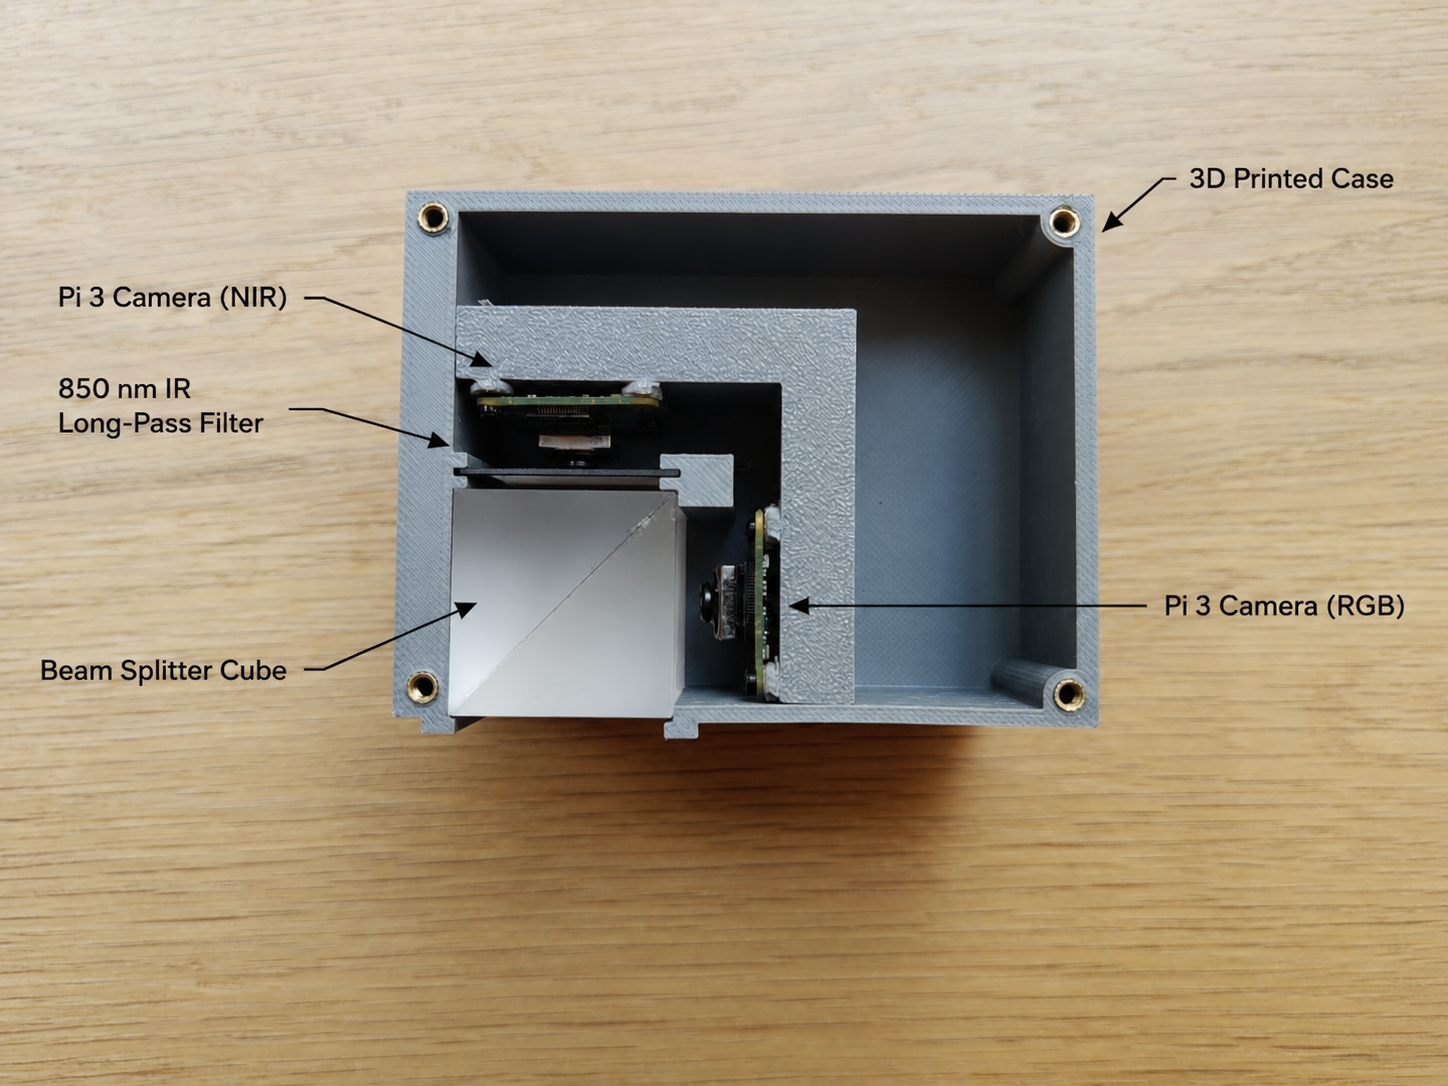
\includegraphics[width=\linewidth]{imgs/device-labeled.png}
        \subcap{(a) Internal layout (lid removed)}
    \end{minipage}
    \hfill
    \begin{minipage}{0.35\textwidth}
        \centering
        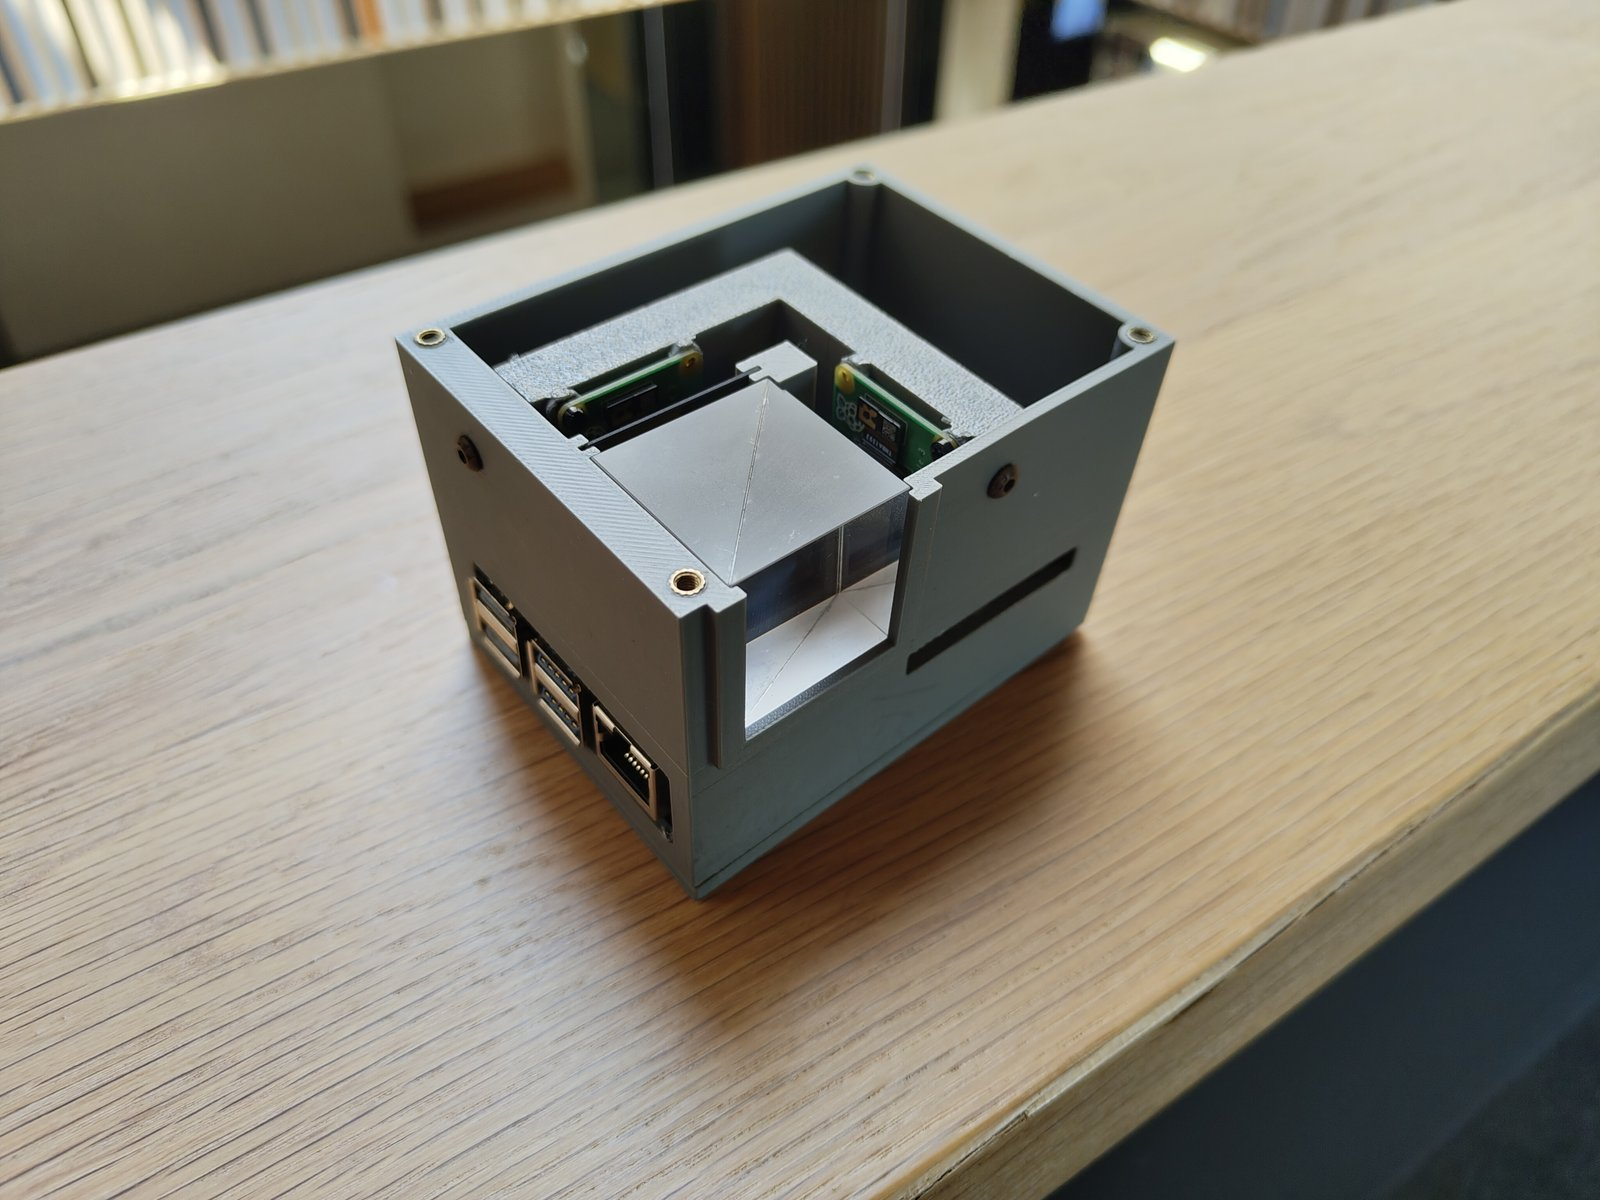
\includegraphics[width=\linewidth]{imgs/rig-internal-photo.jpg}
        \subcap{(b) Assembled rig (lid removed)}
    \end{minipage}
    \caption{The paired-capture rig. A beam-splitter cube feeds the same incoming light to a visible RGB camera and a NIR camera behind an 850\,nm long-pass filter.}
    \label{fig:capture_rig}
\end{figure}

The beam splitter gives both cameras a common optical centre, suppressing the depth-dependent parallax that no 2D warp could remove in a conventional side-by-side rig (Section~\ref{sec:intro_challenges}), at the cost of splitting the available light. With parallax suppressed, a single global homography can align the entire frame regardless of scene depth.

\subsection{Capture campaign}
\label{sec:capture_campaign}

Data was collected over more than 20 hours of cycling around London with the rig mounted on a backpack for hands-free capture (\autoref{fig:rig_deployed}), taking a paired NIR and RGB frame every 5 seconds. Cycling was chosen as it sweeps the rig continuously through diverse urban content. After the filtering and alignment pipeline described below \textbf{12{,}536} usable aligned pairs remained.

\begin{figure}[!htbp]
    \centering
    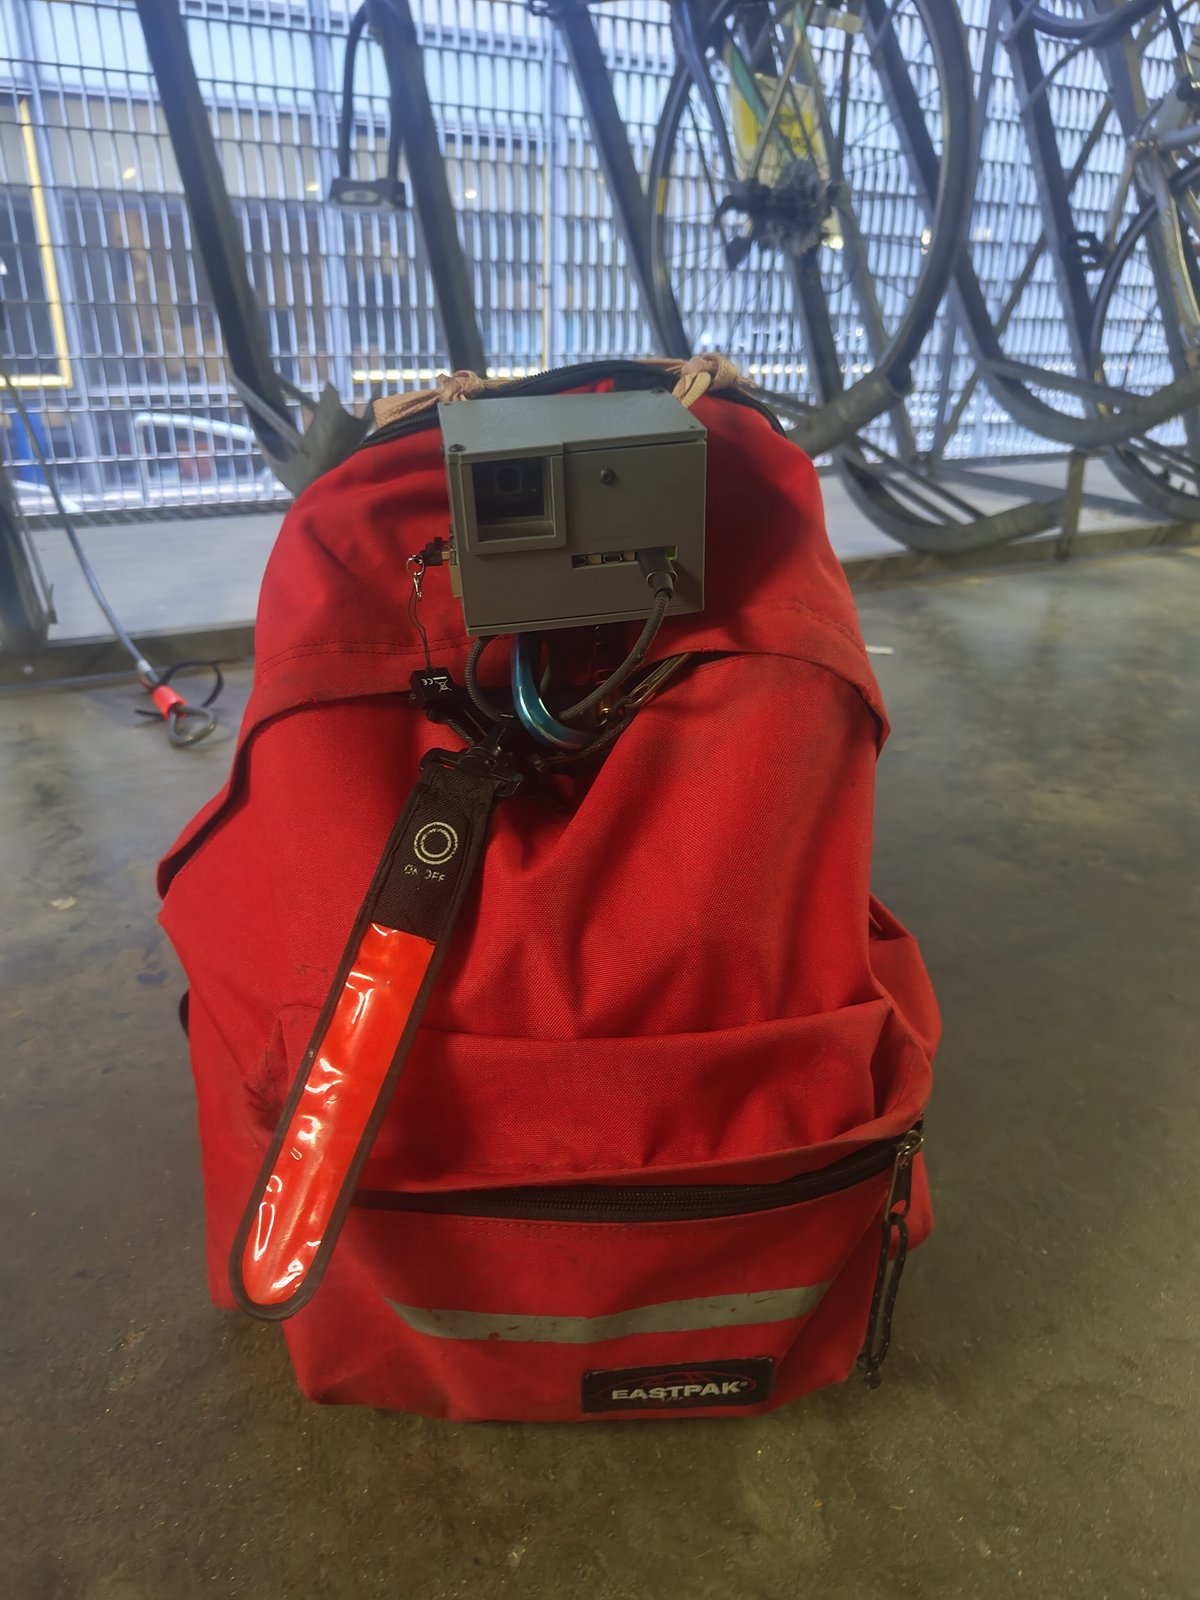
\includegraphics[width=0.5\textwidth]{imgs/rig-deployed.jpg}
    \caption{The capture rig mounted on a backpack for hands-free paired capture while cycling around London.}
    \label{fig:rig_deployed}
\end{figure}

\section{Producing Aligned Pairs}
\label{sec:alignment_pipeline}

Although the beam splitter suppresses parallax, the two optical paths are not pixel-identical. The cameras differ slightly in magnification, principal point and lens distortion, the IR filter shifts the focus of the NIR path, and the mounting can flex a little over a multi-hour ride. A per-pair alignment step absorbs these residual differences. Each raw capture starts as a full-frame RGB/NIR pair (\autoref{fig:pipe_pair}) and goes through the pipeline below. Figures~\ref{fig:pipe_pair}--\ref{fig:pipe_output} show the stages on one example capture.

\begin{figure}[!htbp]
    \centering
    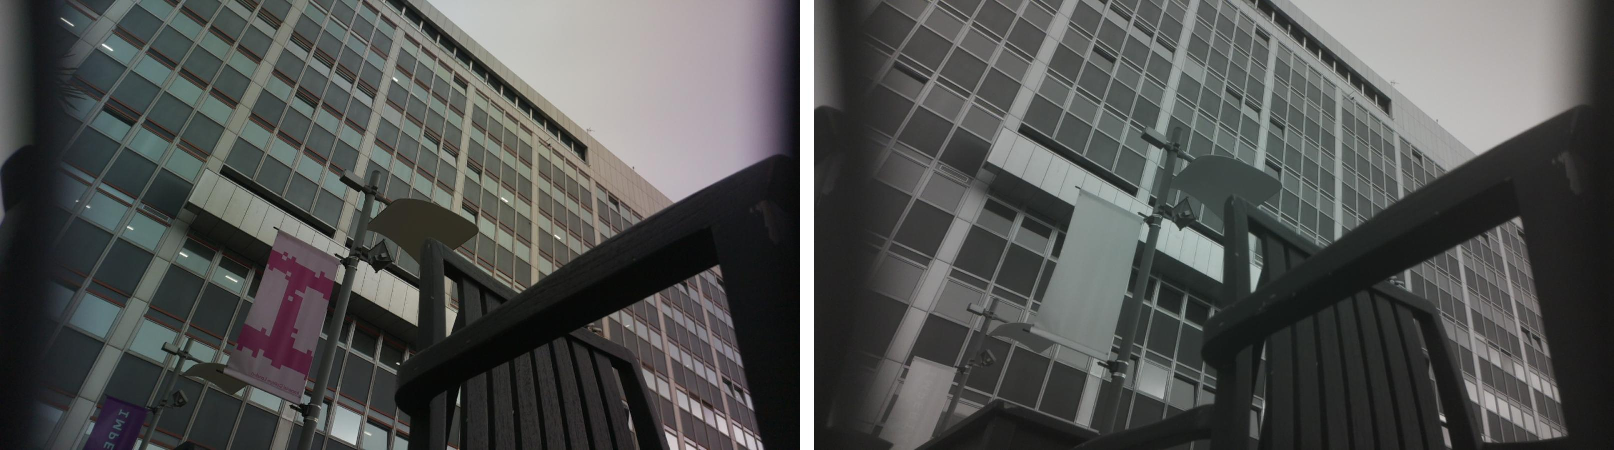
\includegraphics[width=0.9\linewidth]{imgs/pipeline_report/pipeline_01_pair.pdf}
    \caption{The raw captured pair before processing: the full-frame RGB (left) and NIR (right) straight from the two sensors. This is the input to the alignment pipeline.}
    \label{fig:pipe_pair}
\end{figure}

\paragraph{1.~Sharpness filtering.} Cycling introduces motion blur, which corrupts both the supervision target and the feature matching used for alignment. A sharpness score is computed as the variance of the Laplacian of a resized grayscale preview of the RGB frame. Pairs scoring below a threshold of 100 are rejected. The threshold was chosen by inspecting the Laplacian-variance distribution across a sample of captures, where it cleanly separates visibly sharp frames from motion-blurred ones. The example in Figure~\ref{fig:pipe_sharpness} scores 734.3 and is retained.

\begin{figure}[!htbp]
    \centering
    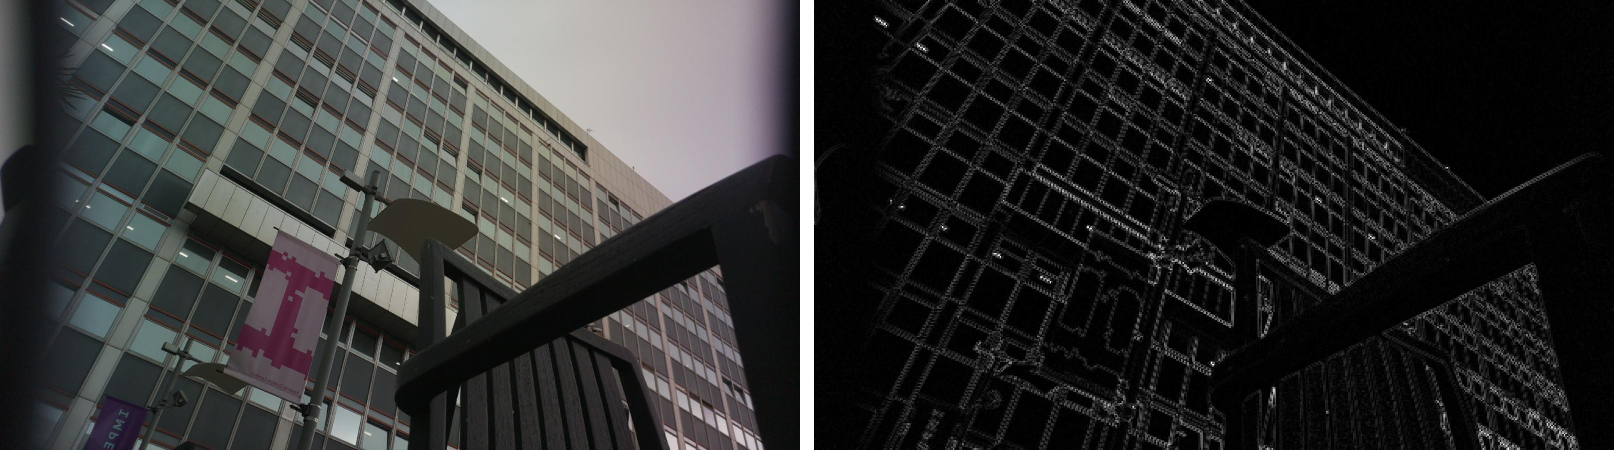
\includegraphics[width=0.9\linewidth]{imgs/pipeline_report/pipeline_02_sharpness.pdf}
    \caption{Sharpness assessment: the RGB frame and its Laplacian response. Frames whose Laplacian variance falls below the threshold (100) are discarded as too blurred for reliable supervision and feature matching.}
    \label{fig:pipe_sharpness}
\end{figure}

\paragraph{2.~Privacy and Anonymisation.} The rig was tilted upwards so pedestrians are not captured at close range, and the $256\times256$ output resolution removes identifying detail. The full privacy measures are set out in Appendix~\ref{app:ethics}.

\paragraph{3.~Square centre-crop.} Both frames are centre-cropped to a common square (\autoref{fig:pipe_crop}). This gives the two images an identical field of view and a consistent geometry for the feature detector.

\begin{figure}[!htbp]
    \centering
    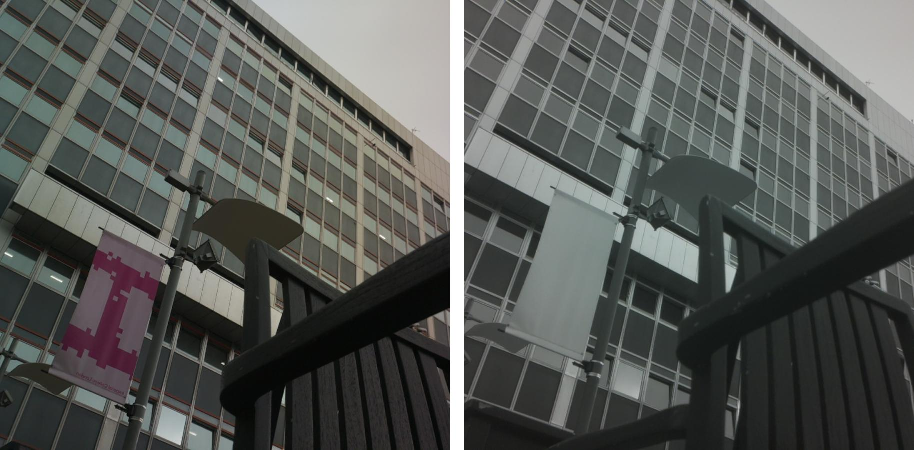
\includegraphics[width=0.7\linewidth]{imgs/pipeline_report/pipeline_03_crop.pdf}
    \caption{Square centre-crop of the RGB (left) and NIR (right) frames to a common field of view.}
    \label{fig:pipe_crop}
\end{figure}

\paragraph{4.~Feature-based alignment.} SIFT keypoints are detected in both crops and matched using Lowe's ratio test. RANSAC then estimates a homography that maps the NIR image onto the RGB image grid, rejecting inconsistent matches as outliers (Listing~\ref{lst:align}). SIFT was preferred over faster binary detectors such as ORB because alignment is a one-off offline step where match quality matters more than speed, and its scale- and rotation-invariant descriptors yield more inliers across the NIR/RGB appearance gap. For the example shown, 199 of 347 accepted SIFT matches are retained as homography inliers (Figure~\ref{fig:pipe_sift}).

\begin{lstlisting}[caption={Feature-based NIR$\rightarrow$RGB alignment: SIFT matching with Lowe's ratio test, followed by a RANSAC homography fit and warp.}, label={lst:align}]
kp_n, des_n = sift.detectAndCompute(nir, None)
kp_r, des_r = sift.detectAndCompute(rgb, None)
matches = matcher.knnMatch(des_n, des_r, k=2)
good = [m for m, n in matches if m.distance < 0.75 * n.distance]  # Lowe ratio
src = np.float32([kp_n[m.queryIdx].pt for m in good])
dst = np.float32([kp_r[m.trainIdx].pt for m in good])
H, inliers = cv2.findHomography(src, dst, cv2.RANSAC, 3.0)
nir_aligned = cv2.warpPerspective(nir, H, (width, height))
\end{lstlisting}

\begin{figure}[!htbp]
    \centering
    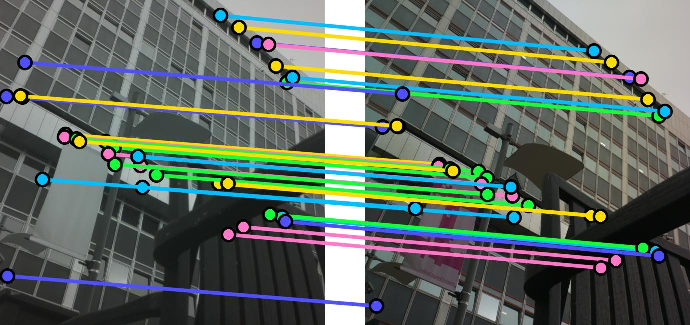
\includegraphics[width=0.9\linewidth]{imgs/pipeline_report/pipeline_04_sift.pdf}
    \caption{SIFT inlier correspondences (after Lowe's ratio test and RANSAC) used to estimate the NIR$\rightarrow$RGB homography for one capture: 199 inliers from 347 accepted matches.}
    \label{fig:pipe_sift}
\end{figure}

\paragraph{5.~Warp, overlap crop, resize, and export.} The NIR image is warped onto the RGB coordinate grid using the estimated homography. Both images are then cropped to their valid overlap region, centre-cropped to a common square, and resized to the $256\times256$ resolution used for storage and training. Captures that yield too few inliers, or a degenerate homography, are discarded at this stage. Figure~\ref{fig:pipe_output} shows a final homography-aligned pair.

\begin{figure}[!htbp]
    \centering
    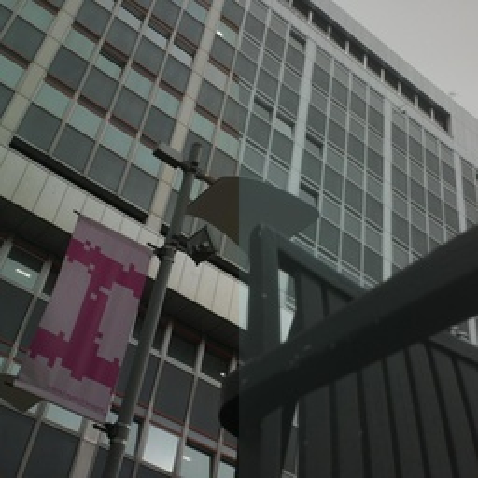
\includegraphics[width=0.9\linewidth]{imgs/pipeline_report/pipeline_05_output.pdf}
    \caption{Image pair, resized to the final $256\times256$ resolution and shown as a half-RGB (left), half-NIR (right) composite.}
    \label{fig:pipe_output}
\end{figure}

Applying this pipeline to the capture campaign produced the 12{,}536 retained pairs used for training and evaluation. The final protocol uses a fixed image-level 80/10/10 split, giving 10{,}028 training, 1{,}253 validation and 1{,}255 test pairs. 

\section{Translator Model: NAFNet Teacher}
\label{sec:nafnet_teacher}

The translator is NAFNet~\cite{chen2022nafnet}, a 2022 ``simple baselines'' architecture for image restoration, here configured for paired NIR$\rightarrow$RGB translation and trained as the high-quality \emph{teacher} for the project. It was chosen over a Pix2Pix-style U-Net for the reasons set out in Section~\ref{sec:architecture_choice}. This section documents the model as built. The reported configuration is the width-64 variant, with 116\,M parameters. \autoref{fig:nafnet_arch} shows the overall topology: a U-shaped encoder--bottleneck--decoder with additive skip connections, built entirely from the NAFBlock of \autoref{fig:nafblock}.

\begin{figure}[!htbp]
\centering
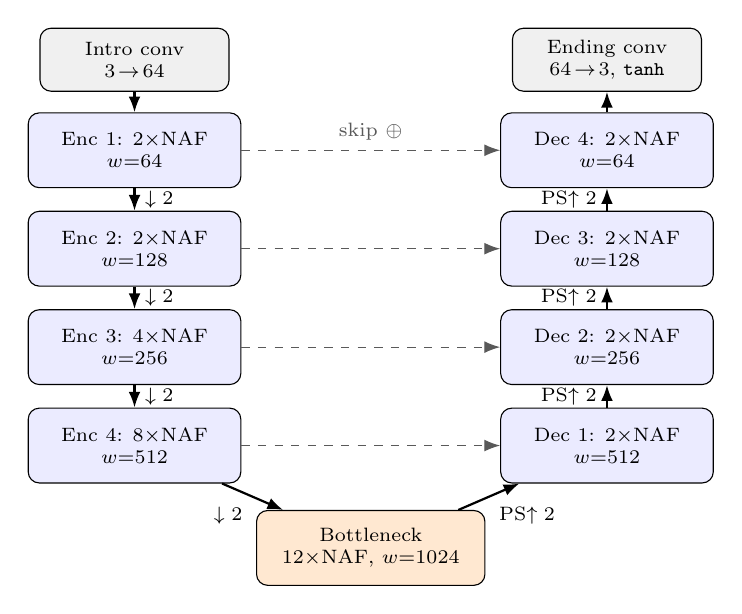
\begin{tikzpicture}[
  font=\scriptsize,
  stage/.style={rectangle, rounded corners, draw, fill=blue!8, minimum width=2.7cm, minimum height=0.95cm, align=center},
  mid/.style={rectangle, rounded corners, draw, fill=orange!18, minimum width=2.9cm, minimum height=0.95cm, align=center},
  io/.style={rectangle, rounded corners, draw, fill=gray!12, minimum width=2.4cm, minimum height=0.8cm, align=center},
  ar/.style={-{Latex[length=2mm]}, thick},
  sk/.style={-{Latex[length=2mm]}, dashed, gray!70!black}
]
\node[io]    (intro) at (0,1.15) {Intro conv\\$3\!\to\!64$};
\node[stage] (e1) at (0,0)      {Enc 1: $2\times$NAF\\$w{=}64$};
\node[stage] (e2) at (0,-1.25)  {Enc 2: $2\times$NAF\\$w{=}128$};
\node[stage] (e3) at (0,-2.5)   {Enc 3: $4\times$NAF\\$w{=}256$};
\node[stage] (e4) at (0,-3.75)  {Enc 4: $8\times$NAF\\$w{=}512$};
\node[mid]   (mid) at (3,-5.05)  {Bottleneck\\$12\times$NAF, $w{=}1024$};
\node[stage] (d1) at (6,-3.75)  {Dec 1: $2\times$NAF\\$w{=}512$};
\node[stage] (d2) at (6,-2.5)   {Dec 2: $2\times$NAF\\$w{=}256$};
\node[stage] (d3) at (6,-1.25)  {Dec 3: $2\times$NAF\\$w{=}128$};
\node[stage] (d4) at (6,0)      {Dec 4: $2\times$NAF\\$w{=}64$};
\node[io]    (end) at (6,1.15)  {Ending conv\\$64\!\to\!3$, \texttt{tanh}};
\draw[ar] (intro) -- (e1);
\draw[ar] (e1) -- (e2) node[midway,right]{$\downarrow2$};
\draw[ar] (e2) -- (e3) node[midway,right]{$\downarrow2$};
\draw[ar] (e3) -- (e4) node[midway,right]{$\downarrow2$};
\draw[ar] (e4) -- (mid) node[midway,below left]{$\downarrow2$};
\draw[ar] (mid) -- (d1) node[midway,below right]{PS$\uparrow2$};
\draw[ar] (d1) -- (d2) node[midway,left]{PS$\uparrow2$};
\draw[ar] (d2) -- (d3) node[midway,left]{PS$\uparrow2$};
\draw[ar] (d3) -- (d4) node[midway,left]{PS$\uparrow2$};
\draw[ar] (d4) -- (end);
\draw[sk] (e1.east) -- (d4.west) node[midway,above]{skip $\oplus$};
\draw[sk] (e2.east) -- (d3.west);
\draw[sk] (e3.east) -- (d2.west);
\draw[sk] (e4.east) -- (d1.west);
\end{tikzpicture}
\caption[NAFNet teacher architecture.]{The NAFNet teacher: a U-shaped encoder--bottleneck--decoder of NAFBlocks. Stride-2 convolutions downsample in the encoder, PixelShuffle (PS) upsamples in the decoder, and encoder features are \emph{added} ($\oplus$) into the matching decoder stage. The input is 3-channel NIR, the output 3-channel RGB in $[-1,1]$.}
\label{fig:nafnet_arch}
\end{figure}

\subsection{The NAFBlock}
\label{sec:nafnet_block_structure}

The network's only building block is the NAFBlock (\autoref{fig:nafblock}), and it contains \emph{no} conventional activation function. In place of a ReLU or GELU it uses a \emph{SimpleGate}: the feature map is split in half along the channel dimension and the two halves are multiplied elementwise.

\begin{lstlisting}[caption={The SimpleGate used in place of a nonlinear activation: the channels are split in half and multiplied elementwise.}, label={lst:simplegate}]
class SimpleGate(nn.Module):
    def forward(self, x):
        a, b = x.chunk(2, dim=1)   # split channels in half
        return a * b               # gate, no ReLU / GELU
\end{lstlisting}

Each block has two residual sub-blocks: a gated convolutional block (LayerNorm, $1{\times}1$ channel expansion, depthwise $3{\times}3$ convolution, SimpleGate, a lightweight squeeze-and-excitation channel reweighting, and a $1{\times}1$ projection) and a gated feed-forward block (LayerNorm, $1{\times}1$, SimpleGate, $1{\times}1$). Each sub-block is added back to its input through a learnable per-channel scale ($\beta$, $\gamma$) initialised to zero, so every block starts as an identity map and the deep stack trains stably from the first step.

The absence of nonlinear activations matters most for this project. With no saturating activations whose value distribution shifts under quantisation, the block keeps a predictable dynamic range, which eases the INT8 export discussed in Section~\ref{sec:edge_deployment}. It also leaves a small, standard operator set (convolution, layer normalisation, elementwise multiply and pixel shuffle) that exports cleanly to ONNX and the runtimes targeted for the edge device.

\begin{figure}[!htbp]
\centering
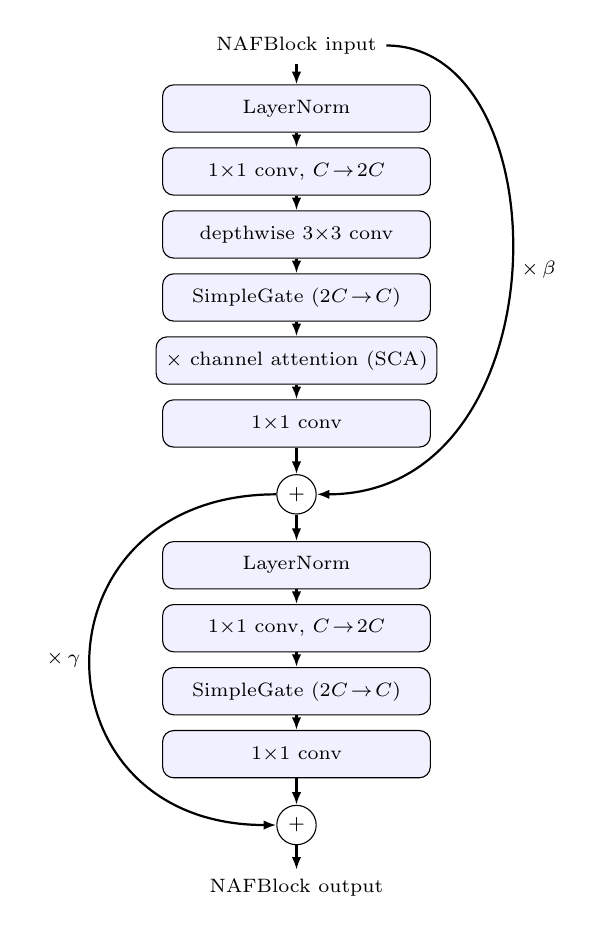
\begin{tikzpicture}[
  font=\scriptsize,
  op/.style={rectangle, rounded corners, draw, fill=blue!6, minimum width=3.4cm, minimum height=0.6cm, align=center},
  add/.style={circle, draw, inner sep=0.5pt, minimum size=0.5cm},
  ar/.style={-{Latex[length=1.6mm]}, thick}
]
\node            (in)  at (0,0)     {NAFBlock input};
\node[op]        (ln1) at (0,-0.8)  {LayerNorm};
\node[op]        (c1)  at (0,-1.6)  {$1{\times}1$ conv, $C\!\to\!2C$};
\node[op]        (dw)  at (0,-2.4)  {depthwise $3{\times}3$ conv};
\node[op]        (sg1) at (0,-3.2)  {SimpleGate ($2C\!\to\!C$)};
\node[op]        (sca) at (0,-4.0)  {$\times$ channel attention (SCA)};
\node[op]        (c3)  at (0,-4.8)  {$1{\times}1$ conv};
\node[add]       (a1)  at (0,-5.7)  {$+$};
\node[op]        (ln2) at (0,-6.6)  {LayerNorm};
\node[op]        (c4)  at (0,-7.4)  {$1{\times}1$ conv, $C\!\to\!2C$};
\node[op]        (sg2) at (0,-8.2)  {SimpleGate ($2C\!\to\!C$)};
\node[op]        (c5)  at (0,-9.0)  {$1{\times}1$ conv};
\node[add]       (a2)  at (0,-9.9)  {$+$};
\node            (out) at (0,-10.7) {NAFBlock output};
\draw[ar] (in)--(ln1); \draw[ar](ln1)--(c1); \draw[ar](c1)--(dw); \draw[ar](dw)--(sg1);
\draw[ar](sg1)--(sca); \draw[ar](sca)--(c3); \draw[ar](c3)--(a1);
\draw[ar](a1)--(ln2); \draw[ar](ln2)--(c4); \draw[ar](c4)--(sg2); \draw[ar](sg2)--(c5);
\draw[ar](c5)--(a2); \draw[ar](a2)--(out);
\draw[ar] (in.east) .. controls (3.4,0) and (3.4,-5.7) .. (a1.east) node[pos=0.5,right]{$\times\,\beta$};
\draw[ar] (a1.west) .. controls (-3.4,-5.7) and (-3.4,-9.9) .. (a2.west) node[pos=0.5,left]{$\times\,\gamma$};
\end{tikzpicture}
\caption{The NAFBlock: a gated convolutional sub-block followed by a gated feed-forward sub-block, with no nonlinear activation. The SimpleGate halves the channels and multiplies them. Learnable per-channel scales $\beta,\gamma$ (initialised to zero) gate each residual so the block starts as an identity map.}
\label{fig:nafblock}
\end{figure}

\subsection{Backbone configuration}
\label{sec:nafnet_backbone}

The encoder has four stages of [2, 2, 4, 8] NAFBlocks at channel widths [64, 128, 256, 512]; each stage is followed by a stride-2 $2{\times}2$ convolution that halves resolution and doubles the channel count. A bottleneck of 12 NAFBlocks runs at width 1024. The decoder mirrors the encoder with [2, 2, 2, 2] blocks, upsampling with PixelShuffle$\times$2. Encoder features are \emph{added} into the matching decoder stage rather than concatenated, which keeps channel counts, and therefore parameters, down. An intro $3{\times}3$ convolution lifts the 3-channel NIR input to width 64, and an ending $3{\times}3$ convolution maps back to 3 channels, followed by a \texttt{tanh} into $[-1,1]$. NAFNet's optional global input$\rightarrow$output residual is disabled, because NIR and RGB are different modalities and adding the input back would force the network to encode all colour as a delta on the NIR. \autoref{tab:teacher_config} summarises the configuration.

\begin{table}[!htbp]
\centering
\footnotesize
\begin{tabular}{ll}
\hline
\textbf{Component} & \textbf{Setting} \\
\hline
Generator & NAFNet, width 64 (116\,M params) \\
Encoder stages & $[2,2,4,8]$ blocks @ widths $[64,128,256,512]$ \\
Bottleneck & 12 blocks @ width 1024 \\
Decoder stages & $[2,2,2,2]$ blocks, PixelShuffle$\times2$ \\
Skip connections & additive (encoder $\to$ decoder) \\
Input / output & 3-ch NIR / 3-ch RGB, $256\times256$, \texttt{tanh}$\to[-1,1]$ \\
Global residual & disabled \\
Discriminator & $70\times70$ PatchGAN; GAN weight 0.3 (30-epoch warmup) \\
Feature-map ensemble & DINOv2/CLIP/ResNet-50 weights 40/20/5 (30-epoch warmup) \\
Optimiser & Adam; lr $2\times10^{-5}$; G $\beta(0.9,0.99)$, D $\beta(0.5,0.999)$ \\
Batch / precision & 1 / full precision (FP32), gradient clip 0.5 \\
Schedule & 200 epochs, trained from scratch (single stage) \\
Checkpoint selection & best validation CLIP cosine similarity \\
\hline
\end{tabular}
\caption{NAFNet teacher configuration for the run \texttt{ablation\_15b\_l1boost\_split42\_s2}. Epoch 199 was selected by the highest validation CLIP ViT-B/32 cosine similarity.}
\label{tab:teacher_config}
\end{table}

\subsection{Training objective}
\label{sec:teacher_loss}

The final teacher augments the conventional pixel-plus-adversarial recipe with a \emph{foundation-model feature-matching ensemble} (whose components are ablated individually in Chapter~\ref{ch:results}). Alongside an L1 colour term (weight 20), an MS-SSIM structural term (weight 3) and a lightly weighted adversarial PatchGAN term (weight 0.3, linearly warmed up over the first 30 epochs), most of the semantic supervision comes from matching the deep features of the prediction and the ground truth across three frozen pretrained backbones, namely DINOv2 ViT-S/14, CLIP ViT-B/32 and ResNet-50, each contributing a feature-space loss computed at $224\times224$. The feature-matching ensemble is also linearly warmed up over the first 30 epochs. Only the VGG-perceptual term is switched off (\autoref{tab:teacher_loss}). Unlike the multi-stage baseline, the teacher is trained from scratch in a single stage. The comparatively strong L1 anchor keeps the pixel-level signal competitive while the foundation-feature gradient is introduced, which stabilises single-stage convergence.

The rationale for replacing the single VGG perceptual term with this ensemble is set out in Section~\ref{sec:loss_design}. In keeping with that objective, checkpoints are selected on validation CLIP cosine similarity rather than PSNR.

\begin{table}[!htbp]
\centering
\footnotesize
\begin{tabular}{lcl}
\hline
\textbf{Loss term} & \textbf{Weight} & \textbf{Role} \\
\hline
L1 (pixel) & 20 & global colour anchor \\
MS-SSIM & 3 & structural similarity \\
Adversarial (LSGAN, $70\times70$ PatchGAN) & 0.3 & realism (30-epoch warmup) \\
DINOv2 ViT-S/14 feature match & 40 & semantic, self-supervised features \\
CLIP ViT-B/32 feature match & 20 & vision--language semantic features \\
ResNet-50 feature match & 5 & ImageNet convolutional features \\
VGG perceptual & 0 & disabled (used only by the baseline, Ch.~\ref{ch:results}) \\
\hline
\end{tabular}
\caption{The final teacher's training objective: L1 and MS-SSIM terms, a lightly weighted adversarial PatchGAN term, and a frozen foundation-model feature-matching ensemble. Each feature term is a feature-space loss computed at $224\times224$ on its backbone; the foundation-feature terms are linearly warmed up over the first 30 epochs.}
\label{tab:teacher_loss}
\end{table}

\subsection{Optimisation and convergence}
\label{sec:nafnet_training}

Training operates on $256\times256$ paired crops. NIR and RGB are augmented jointly with geometric transforms (random scale $[0.9,1.15]$, crop, horizontal flip, rotation up to $10^\circ$); the NIR input additionally receives photometric jitter (brightness $\pm0.2$, gamma $[0.8,1.2]$) so the translator is robust to the exposure variation that alignment cannot remove. Both tensors are normalised to $[-1,1]$.

Optimisation uses Adam (generator $\beta=(0.9,0.99)$, discriminator $\beta=(0.5,0.999)$) at a learning rate of $2\times10^{-5}$ in full precision; automatic mixed precision is disabled because the frozen foundation-model feature extractors were numerically more stable in FP32. Gradient clipping is set to 0.5 and the batch size to 1, which is memory-bound at $256^2$ with the 116\,M-parameter generator and three frozen feature extractors resident on the GPU. The adversarial and foundation-feature weights are ramped to their targets over the first 30 epochs. The teacher is trained from scratch in a single stage for 200 epochs. The translator is implemented in PyTorch, with version control via Git and experiment tracking through Weights \& Biases. Training was run mainly on Google Cloud \texttt{g2-standard-8} spot instances (NVIDIA L4), with up to four used in parallel for ablation sweeps, and on Imperial DoC workstations equipped with NVIDIA RTX~4080 (16\,GB), RTX~5090 (32\,GB) and RTX~6000 (48\,GB each). Checkpoints and training metrics are logged to Weights \& Biases for artefact retrieval and reproducibility.

\autoref{fig:training_curves} tracks the final teacher run. At the selected epoch 199 checkpoint, validation DINOv2-S cosine similarity is 0.9517, CLIP ViT-B/32 cosine similarity is 0.9090, PSNR is 26.497\,dB, SSIM is 0.8278 and LPIPS is 0.0985. PSNR is not the training target. The recipe trades a little pixel fidelity for stronger feature-space agreement, the quantity the downstream panel responds to. The checkpoint with the highest validation CLIP cosine similarity was selected for downstream evaluation. \autoref{fig:sample_grid} shows representative held-out test translations.

\begin{figure}[!htbp]
\centering
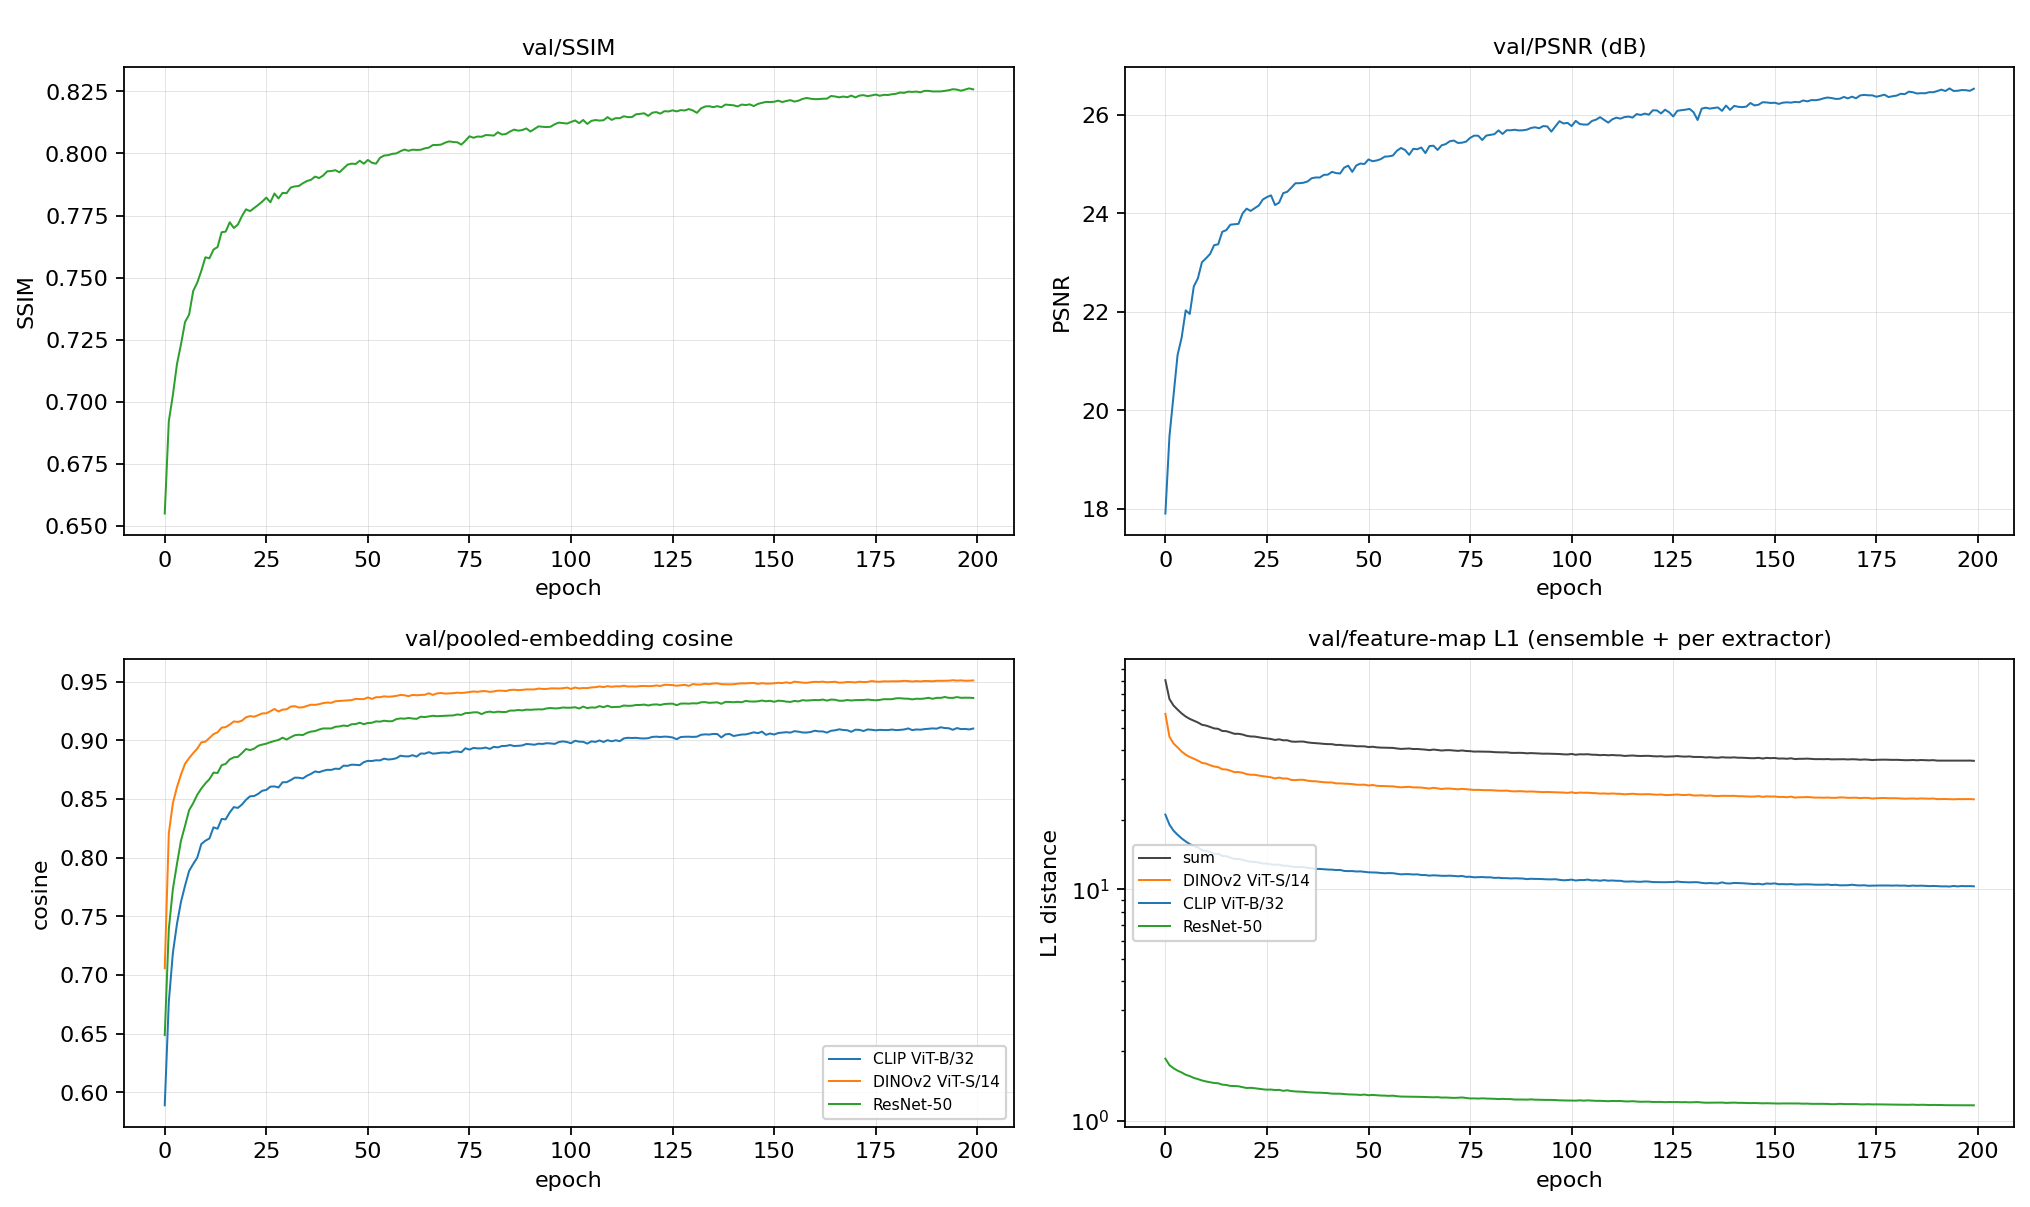
\includegraphics[width=\linewidth]{imgs/l1boost_curves.png}
\caption[Final-teacher validation metrics during training.]{Final-teacher validation metrics during training for \texttt{ablation\_15b\_l1boost\_split42\_s2} (foundation-ensemble objective; 200 epochs from scratch). Top left: SSIM and PSNR progress. Bottom left: pooled-embedding cosine similarity across three evaluators (CLIP ViT-B/32, DINOv2 ViT-S/14, ResNet-50). Bottom right: feature-map L1 distance showing alignment across extractors. Epoch 199 was selected by highest validation CLIP ViT-B/32 cosine similarity.}
\label{fig:training_curves}
\end{figure}

\begin{figure}[!htbp]
\centering
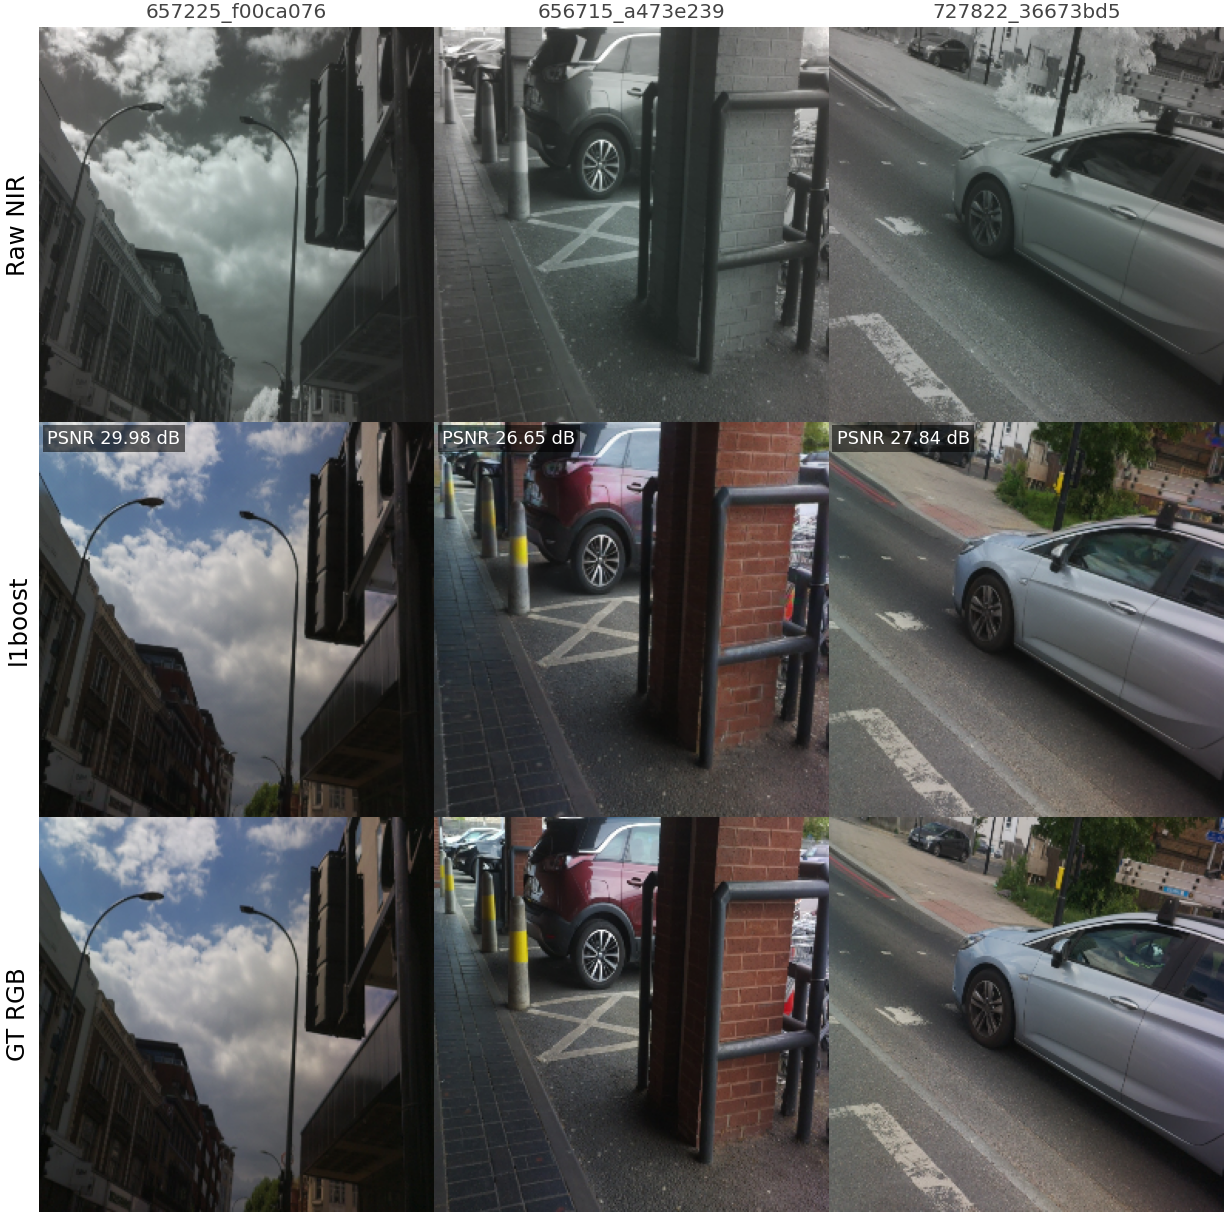
\includegraphics[width=\linewidth]{imgs/grid_22.png}
\caption{Five examples from the final foundation-ensemble teacher. The teacher recovers plausible colour and preserves scene structure across varied urban content.}
\label{fig:sample_grid}
\end{figure}

\section{Edge Deployment Path for the Raspberry Pi 5}
\label{sec:edge_deployment}

The teacher of Section~\ref{sec:nafnet_teacher} is not the intended deployment model; at 116\,M parameters it is too large for the Raspberry~Pi~5 target. The deployment path follows the teacher--student strategy of Section~\ref{sec:edge_student}: a compact student is distilled, exported and quantised to mixed INT8. The resulting artefact runs on the Pi~5 CPU, and a second export path targets the Hailo-8L neural accelerator on the Pi AI HAT+. Both are benchmarked on the device in Section~\ref{sec:impl_ondevice} and Section~\ref{sec:res_edge}.

\subsection{Distilled student}
\label{sec:impl_student}

A compact NAFNet is distilled from the width-64 teacher to target the Raspberry~Pi~5 CPU. It keeps the teacher's NAFNet block structure of the activation-free SimpleGate plus channel attention, so it inherits the same quantisation-friendly, export-clean operator set, and reduces only width and block depth. With width~16 and the shallowest depth (encoder blocks $[1,1,1,2]$, two middle blocks, decoder blocks $[1,1,1,1]$) it has only 1.7\,M parameters, roughly $1/67$ of the teacher, small enough for near-interactive inference on the CPU runtimes (Section~\ref{sec:impl_export}).

\begin{table}[!htbp]
\centering
\footnotesize
\begin{tabular}{lccc}
\hline
 & \textbf{CPU student} & \textbf{NPU student} & \textbf{Teacher} \\
 & \textbf{(width-16)} & \textbf{(width-32)} & \textbf{(width-64)} \\
\hline
Width          & 16          & 32          & 64          \\
Encoder blocks & $[1,1,1,2]$ & $[1,1,2,4]$ & $[2,2,4,8]$ \\
Middle blocks  & 2           & 4           & 12          \\
Decoder blocks & $[1,1,1,1]$ & $[1,1,1,1]$ & $[2,2,2,2]$ \\
Parameters     & 1.7\,M      & 11.6\,M     & 116\,M      \\
\hline
\end{tabular}
\caption{The distilled students against the teacher. Both students preserve the teacher's NAFNet block type and reduce only width and depth; the width-16 student is shaped for the Pi~5 CPU, and the larger width-32 variant for the Hailo-8L NPU (Section~\ref{sec:impl_hailo}).}
\label{tab:student_arch}
\end{table}

The student is trained to reproduce the teacher's outputs on the same data. The dominant term is a pixel-level distillation loss to the teacher's RGB output, with a smaller ground-truth L1 anchor and several frozen feature losses, optimising for downstream-representation fidelity rather than pixel mimicry alone (\autoref{tab:student_loss}). The teacher-output term is weighted more heavily than the ground-truth anchor to keep colour tied to measured RGB and limit amplification of teacher artefacts. The selected feature-KD student, \texttt{student\_l1b\_c\_featkd}, was selected at epoch 99 by validation CLIP cosine similarity 0.8585.
\pagebreak

\begin{table}[!htbp]
\centering
\footnotesize
\begin{tabular}{lcl}
\hline
\textbf{Loss term} & \textbf{Weight} & \textbf{Role} \\
\hline
Teacher-output L1 (distillation) & 50 & match the supervising teacher's RGB output \\
Ground-truth L1 & 5 & light colour anchor to real RGB \\
DINOv2 ViT-S/14 feature match & 40 & semantic, self-supervised features \\
CLIP ViT-B/32 feature match & 20 & vision--language semantic features \\
ResNet-50 feature match & 5 & ImageNet convolutional features \\
SegFormer-B0 ADE20K feature match & 15 & segmentation-sensitive features \\
DepthAnything-Small feature match & 10 & geometry-sensitive features \\
Teacher feature-KD match & 0.5 & match student and teacher feature representations \\
\hline
\end{tabular}
\caption{Training objective for the selected \texttt{student\_l1b\_c\_featkd} run. The teacher output is the dominant target, with a light ground-truth anchor, downstream-feature terms and an additional feature-KD term between student and teacher outputs.}
\label{tab:student_loss}
\end{table}

\begin{lstlisting}[caption={The student distillation objective: a dominant teacher-output L1 term, a light ground-truth anchor, and DINOv2/CLIP feature-matching terms.}, label={lst:distill}]
loss = (50.0 * l1(student_out, teacher_out)
        + 5.0 * l1(student_out, rgb_gt)
        + 40.0 * dinov2_feat(student_out, rgb_gt)
        + 20.0 * clip_feat(student_out, rgb_gt)
        + 5.0 * resnet_feat(student_out, rgb_gt)
        + 15.0 * segformer_feat(student_out, rgb_gt)
        + 10.0 * depth_feat(student_out, rgb_gt)
        + 0.5 * feature_kd(student_out, teacher_out))
\end{lstlisting}

\subsection{Export and quantisation}
\label{sec:impl_export}

All quantisation in this project is post-training, and no quantisation-aware training is used (Section~\ref{sec:quantisation}). A single FP32 PyTorch checkpoint is exported to the two runtimes representative of the Pi~5 software stack: ONNX Runtime, and LiteRT (formerly TFLite) executed through the XNNPACK CPU delegate. Export to ONNX uses opset 17 with a dynamic batch axis. Each runtime is benchmarked in full precision (FP32) and in INT8, with two ONNX INT8 variants compared: post-training static quantisation and a per-operator quantise/dequantise (Q/DQ) graph.

The calibration reader streams 100 representative NIR frames drawn deterministically from the seed-42 training split, preprocessed to the training range, and uses per-channel weight quantisation with MinMax activation ranges. With no saturating nonlinearities in the NAFBlock (Section~\ref{sec:nafnet_block_structure}), there is no activation clipping to calibrate around. A few structural operators still lack an INT8 kernel and are left in FP32, so the artefacts are a mixed INT8 rather than fully integer. In the ONNX path this is the PixelShuffle upsampling, which appears as a \texttt{DepthToSpace} node with no INT8 kernel at opset 17; the convolutions feeding it are excluded alongside it, so the optimiser does not strand them between quantise/dequantise pairs. In the LiteRT path the LayerNorm reductions remain in FP32 for the same reason.

The TFLite export was first produced with onnx2tf, but its NCHW$\rightarrow$NHWC layout pass mis-shaped the LayerNorm reduction tensors and broke the XNNPACK delegate. The export was therefore moved to Google's litert-torch, which lowers directly from the PyTorch graph and avoids the layout conversion entirely. The final LiteRT mixed-INT8 artefact is deterministic, occupies 2.3\,MB and retains positive gap closure on all five primary tasks. It executes through XNNPACK on the Pi's ARM CPU, and the measured runtime is reported in Section~\ref{sec:impl_ondevice}.

\subsection{Hailo-8L NPU export}
\label{sec:impl_hailo}

The Raspberry Pi AI HAT+ adds a Hailo-8L neural accelerator to the Pi~5, so a second export path was built to run the student on the NPU rather than the CPU. The Hailo toolchain does not accept the LiteRT or ONNX-Runtime artefacts directly. The FP32 ONNX student is recompiled to a Hailo Executable Format (HEF) file with the Hailo Dataflow Compiler 3.33.1 targeting the hailo8l architecture, which parses the graph, quantises it to INT8 from the same 100-frame calibration set, and allocates the network across the accelerator clusters.

Three operator issues had to be resolved before the graph would compile, and each was fixed without changing the network numerically. First, the PyTorch ONNX export omitted the explicit kernel shape on the convolutions, which the parser requires, so the attribute was restored from the weight tensors. Second, the NAFNet SimpleGate, a channel split followed by an element-wise multiply, is not a supported pattern, so it was rewritten as two $1\times1$ identity-selector convolutions feeding the same multiply, an exact reformulation. Third, the global average pooling in the channel-attention blocks could not be quantised directly because its reduction range was too large, so it was decomposed into a two-stage reduction. With these fixes both the width-16 student and the larger width-32 student variant (11.6\,M parameters; configuration in \autoref{tab:student_arch}) compiled cleanly, into HEF files of 17.7 and 50.4\,MB respectively, each taking a UINT8 $256\times256\times3$ input and producing a UINT8 output of the same shape. The cost of this path is its fragility: the surgery is specific to this operator set and compiler version, and the compiler ships only inside the vendor container rather than as a public package.

\subsection{On-device performance}
\label{sec:impl_ondevice}

The selected student was benchmarked on the Raspberry~Pi~5, on the CPU through LiteRT and on the Hailo-8L NPU. On the CPU the mixed-INT8 student runs at 5.05\,FPS measured at the model call, and on the NPU the same student runs at 27.2\,FPS with a 36.3\,ms hardware latency. Both backends meet the 5\,FPS target, the model footprint stays well inside the Pi's 8\,GB with no swap, and a sustained NPU run showed no thermal throttling. Section~\ref{sec:res_edge} reports the full figures and the requirement decisions.
 % Implementation
\doublespacing % Do not change - required

\chapter{Test Plan and Verification}
\label{ch:testplan}

%%%%%%%%%%%%%%%%%%%%%%%%%%%%%%%%%%%%%%%
% IMPORTANT
\begin{spacing}{1} %THESE FOUR
\minitoc % LINES MUST APPEAR IN
\end{spacing} % EVERY
\thesisspacing % CHAPTER
% COPY THEM IN ANY NEW CHAPTER
%%%%%%%%%%%%%%%%%%%%%%%%%%%%%%%%%%%%%%%

This chapter defines verification of the dataset, translator, evaluation harness and deployment-target student. Each requirement in Chapter~\ref{ch:requirements} is linked to a repeatable test and acceptance condition. Numerical outcomes are kept in Chapter~\ref{ch:results}. This chapter describes how those numbers are produced.

\section{Verification Matrix}
\label{sec:test_matrix}

\autoref{tab:test_matrix} links the requirements and success criteria to the tests used to verify them. Tests T1--T5 cover the translator and dataset, while T6--T8 cover export and deployment.

\begin{table}[H]
\centering
\scriptsize
\setlength{\tabcolsep}{3pt}
\begin{tabular}{p{0.07\linewidth}p{0.13\linewidth}p{0.38\linewidth}p{0.32\linewidth}}
\hline
\textbf{Test} & \textbf{Requirement} & \textbf{Procedure} & \textbf{Acceptance condition} \\
\hline
T1 & F1 & Run every test image through the selected checkpoint and validate output shape, type and range. & One three-channel output at the input resolution for every sample, with no failed inference. \\
T2 & F2, S1 & Audit pair integrity and residual NIR/RGB alignment before training or evaluation. & Every listed pair is readable and matched, split provenance is frozen, and alignment failures are removed and reported. \\
T3 & F3 & Repeat inference on the same inputs with the same checkpoint and runtime. & Repeated 8-bit outputs are identical for a fixed runtime. \\
T4 & F4 & Load the exported model in each target runtime and pass native preprocessed NIR frames through the complete interface. & The runtime accepts the documented input convention and returns standard 8-bit RGB without downstream changes. \\
T5 & N3, S2 & Evaluate image quality and the frozen downstream panel on the held-out test images. & Positive gap closure on at least three of five tasks, with no task below its raw-NIR baseline. \\
T6 & N1, S3 & Benchmark the selected student's model inference on the Raspberry~Pi~5 at $256\times256$. & Mean inference latency no greater than 200\,ms per frame, equivalent to at least 5\,FPS. \\
T7 & N2 & Record artefact size, peak resident memory and swap activity during sustained inference. & The model loads and runs without out-of-memory failure or swapping while meeting T6. \\
T8 & F2, N2 & Compare PyTorch, exported FP32 and INT8 outputs on the same inputs. & FP32 export remains numerically close to PyTorch; INT8 retains the S2 acceptance condition and its quality loss is reported. \\
\hline
\end{tabular}
\caption{Traceability from project requirements to verification tests.}
\label{tab:test_matrix}
\end{table}


\section{Downstream Agreement}
\label{sec:test_downstream}

The main evaluation runs a panel of frozen RGB-pretrained models on raw NIR, translated RGB and native RGB. Native-RGB predictions act as a reference for model behaviour, not as human-labelled ground truth. The resulting numbers measure agreement with the model's RGB behaviour and must not be described as absolute task accuracy.

\begin{table}[H]
\centering
\scriptsize
\setlength{\tabcolsep}{3pt}
\begin{tabular}{lll}
\hline
\textbf{Model} & \textbf{Metric} & \textbf{Task} \\
\hline
YOLOv8m & mAP@0.5, mAP@0.5:0.95 & object detection \\
RT-DETR-L & mAP@0.5, mAP@0.5:0.95 & object detection \\
SegFormer-B0 (ADE20K) & Dice per class & semantic segmentation \\
SegFormer-B0 (Cityscapes) & Dice per class & semantic segmentation \\
DepthAnything-Small & per-image min--max-normalised L1 & depth estimation \\
DINOv2-S & cosine similarity & embedding agreement \\
DINOv2-L & cosine similarity & embedding agreement \\
CLIP-B/16 & cosine similarity & embedding agreement \\
SigLIP2 & cosine similarity & embedding agreement \\
\hline
\end{tabular}
\caption{Evaluation panel: frozen models~\cite{jocher2023yolov8,zhao2024rtdetr,xie2021segformer,yang2024depthanything,oquab2024dinov2,radford2021clip,tschannen2025siglip2} and metrics for measuring gap closure between raw NIR and native RGB.}
\label{tab:downstream_panel_test}
\end{table}

For each evaluator, the primary metric is reduced to the gap-closure statistic defined in Section~\ref{sec:design_evaluation}.

\section{Verification of the Evaluation Harness}
\label{sec:test_harness_verify}

The harness is software under test and is checked independently of the translator. Small deterministic fixtures exercise the aggregation and evaluator-specific edge cases before a model result is trusted.

\begin{table}[!htbp]
\centering
\footnotesize
\begin{tabular}{p{0.23\linewidth}p{0.48\linewidth}p{0.19\linewidth}}
\hline
\textbf{Fixture} & \textbf{Check} & \textbf{Expected result} \\
\hline
NIR identity & Set the translated metric equal to the raw-NIR metric. & Gap closure $=0$. \\
RGB identity & Set the translated metric equal to the RGB metric. & Gap closure $=1$. \\
Negative control & Set the translated metric below the raw-NIR metric. & Negative gap closure. \\
Zero denominator & Set the RGB and NIR metrics equal. & Undefined result, no division error. \\
Detection edge cases & Test empty reference, empty prediction, duplicate candidates and threshold-boundary IoU. & Documented NaN, zero and one-to-one matching behaviour. \\
Ordering & Reorder images without changing values. & Identical aggregate result. \\
\hline
\end{tabular}
\caption{Oracle and edge-case tests used to verify the gap-closure harness.}
\label{tab:harness_tests}
\end{table}

DepthAnything provides an additional behavioural check rather than a proof of correctness. Depth depends strongly on geometry and texture, so a large agreement loss prompts inspection for geometric warping or over-smoothing, but the fixtures in \autoref{tab:harness_tests} remain the direct verification of the aggregation implementation. Running \texttt{python scripts/harness\_unit\_tests.py} produced 10 passing and zero failing tests. Results and logs are retained under \path{experiments/harness_unit_tests/}.


\section{Controlled Robustness Tests}
\label{sec:test_robustness}

The field dataset contains natural variation, but it does not give controlled coverage of every capture condition. A fixed test subset is therefore evaluated after applying deterministic perturbations to the NIR input only. The RGB reference remains unchanged.

\begin{table}[!htbp]
\centering
\footnotesize
\begin{tabular}{lll}
\hline
\textbf{Perturbation} & \textbf{Levels} & \textbf{Purpose} \\
\hline
Exposure gain & $0.8,\ 1.2$ & sensitivity to under- and over-exposure \\
Gamma & $0.8,\ 1.2$ & nonlinear sensor and lighting variation \\
Gaussian blur & $\sigma=1,\ 2$ pixels & focus error and motion blur \\
Gaussian noise & $\sigma=0.01,\ 0.03$ on $[0,1]$ & sensor noise at lower light levels \\
\hline
\end{tabular}
\caption{Controlled NIR-input perturbations used for robustness testing.}
\label{tab:robustness_tests}
\end{table}

The sweep uses the first 200 images of the seed-42 test split, without further shuffling, for the final teacher and selected FP32 student. It reports paired changes in PSNR, LPIPS, CLIP-B/16 cosine and DINOv2-L cosine in \path{experiments/robustness_v1/per_image.csv}. The measured deltas, and the operating envelope they define, are reported in Section~\ref{sec:res_robustness}.

\section{Export and Quantisation Verification}
\label{sec:test_export}

Export is verified before latency is measured. A fixed set of validation NIR images is run through PyTorch FP32, ONNX FP32 and LiteRT FP32. Output shape, range and finite values are checked, followed by mean and maximum absolute differences from PyTorch. Repeated runs on each runtime verify determinism. A visible image grid is also inspected because a small aggregate error can hide a layout or channel-order fault.

The INT8 models are then evaluated on the same final test data as the FP32 student. PSNR, SSIM, LPIPS and downstream gap closure are compared directly with FP32, and the difference is reported rather than described only as visually similar. Calibration uses 100 representative NIR frames from the training split. No test image is used to select ranges, exclude operators or choose between quantisation variants.

The export artefact size and peak resident memory are recorded for every runtime. Peak memory is measured after model loading and during sustained inference, with swap activity checked at the same time. This verifies N2 directly rather than using parameter count as a proxy.


\section{Reproducibility}
\label{sec:test_repro}

Each experiment directory keeps the configuration used for the run, and the evaluation scripts pin the configuration and checkpoint they load, so every reported number can be traced to the model that produced it. The train/validation/test split is derived deterministically from a fixed seed, so the same partition is recovered on every run. Per-image metrics are retained for every evaluation, so aggregate tables, confidence intervals and failure cases can be regenerated without rerunning the downstream models, and the bootstrap settings behind the confidence intervals are stored alongside the per-image data. Package versions are pinned in a frozen environment file, and the training and evaluation commands are encoded in per-experiment run scripts. The deployment commands are collected in Appendix~\ref{app:userguide}.

\section{Test Limitations}
\label{sec:test_limitations}

The downstream panel uses native-RGB model outputs as pseudo-ground truth because the captured dataset has no task annotations. It therefore measures recovery of RGB-model behaviour, not correctness against human labels. The on-device latency figures measure the model call on prepared tensors. Per-frame pre- and post-processing was not separately timed, so the full capture-to-output delay of a deployed pipeline is not tested. The data cover outdoor urban scenes in London and do not establish performance indoors, in other climates or with a different NIR sensor. Controlled perturbations broaden the tested conditions but cannot replace an independent external dataset.
 % Test Plan and Verification
\doublespacing % Do not change - required

\chapter{Results}
\label{ch:results}

%%%%%%%%%%%%%%%%%%%%%%%%%%%%%%%%%%%%%%%
% IMPORTANT
\begin{spacing}{1} %THESE FOUR
\minitoc % LINES MUST APPEAR IN
\end{spacing} % EVERY
\thesisspacing % CHAPTER
% COPY THEM IN ANY NEW CHAPTER
%%%%%%%%%%%%%%%%%%%%%%%%%%%%%%%%%%%%%%%

This chapter reports the results in four parts. First, image-quality metrics act as sanity checks that the translator has not lost basic fidelity (Section~\ref{sec:res_imagequality}), though they are not the main success criterion. Second, downstream metrics across detection, segmentation and embedding spaces ask whether the translated images make frozen RGB-pretrained models behave more like they do on native RGB (Section~\ref{sec:res_downstream}). Third, the teacher ablation study explains how the final recipe was reached, moving from a conventional baseline to the foundation-feature ensemble (Section~\ref{sec:res_ablation}). Finally, the edge section reports the Raspberry~Pi~5 benchmark for the deployed student on both the CPU and the Hailo-8L NPU, and a live on-device demonstration (Section~\ref{sec:res_edge}).

\section{Image Quality}
\label{sec:res_imagequality}

PSNR, SSIM and LPIPS are useful checks that the translator has not lost basic image fidelity, but they are secondary to the downstream behavioural metrics in Section~\ref{sec:res_downstream}. \autoref{tab:res_imagequality} compares raw NIR, the conventional Pix2Pix baseline, the final teacher and the deployment-target student variants. 

\begin{table}[!htbp]
\centering
\scriptsize
\setlength{\tabcolsep}{2.5pt}
\resizebox{\linewidth}{!}{%
\begin{tabular}{lccccc}
\hline
\textbf{Model} & \textbf{PSNR\,(dB), mean [95\% CI]} $\uparrow$ & \textbf{SSIM, mean [95\% CI]} $\uparrow$ & \textbf{LPIPS, mean [95\% CI]} $\downarrow$ & \textbf{Params} & \textbf{Artefact size} \\
\hline
Raw NIR & 16.65 [16.46, 16.84] & 0.656 [0.648, 0.665] & 0.337 [0.330, 0.344] & N/A & N/A \\
Pix2Pix baseline (U-Net) & 24.03 [23.83, 24.24] & 0.752 [0.746, 0.758] & 0.185 [0.180, 0.190] & 54.4\,M & 686.3\,MB checkpoint \\
Teacher (NAFNet-64) & 26.16 [25.91, 26.42] & 0.818 [0.812, 0.824] & 0.103 [0.099, 0.108] & 116\,M & 1{,}425.7\,MB checkpoint \\
Student FP32 (NAFNet-16) & 24.09 [23.86, 24.33] & 0.781 [0.774, 0.787] & 0.146 [0.141, 0.150] & 1.7\,M & 7.1\,MB LiteRT \\
Student mixed-INT8 (NAFNet-16) & 23.57 [23.35, 23.79] & 0.770 [0.763, 0.776] & 0.153 [0.148, 0.158] & 1.7\,M & 2.3\,MB LiteRT \\
\hline
\end{tabular}
}
\caption{Image-quality and artefact-size comparison on the canonical held-out test split. The FP32 student also has a 7.6\,MB ONNX artefact.}
\label{tab:res_imagequality}
\end{table}

The final teacher gives the strongest fidelity result, improving over Pix2Pix by 2.13\,dB PSNR, 0.066 SSIM and 0.082 LPIPS. The width-16 FP32 student trades some of this quality for a $67.3\times$ parameter reduction: relative to the teacher, it loses 2.07\,dB PSNR and 0.037 SSIM, while LPIPS increases by 0.0426. It also matches or beats the Pix2Pix baseline on every pixel and perceptual metric: PSNR ties (24.09 against 24.03), SSIM is higher (0.781 against 0.752) and LPIPS is lower (0.146 against 0.185), all at 1/32 of the parameters. On these traditional metrics the compact student is therefore as good as the GAN baseline, which makes the downstream comparison in Section~\ref{sec:res_downstream} the deciding evidence.

Post-training quantisation introduces a further, measurable quality cost. Relative to the FP32 student, the mixed-INT8 model loses 0.523\,dB PSNR and 0.0114 SSIM, and LPIPS increases by 0.0073. In return, the LiteRT artefact falls from 7.1\,MB to 2.3\,MB. The qualitative examples in \autoref{fig:student_compare_grid} show that the two students preserve the teacher's broad colour and structure on typical cases, while both are somewhat less saturated and detailed than the teacher.

\begin{figure}[!htbp]
\centering
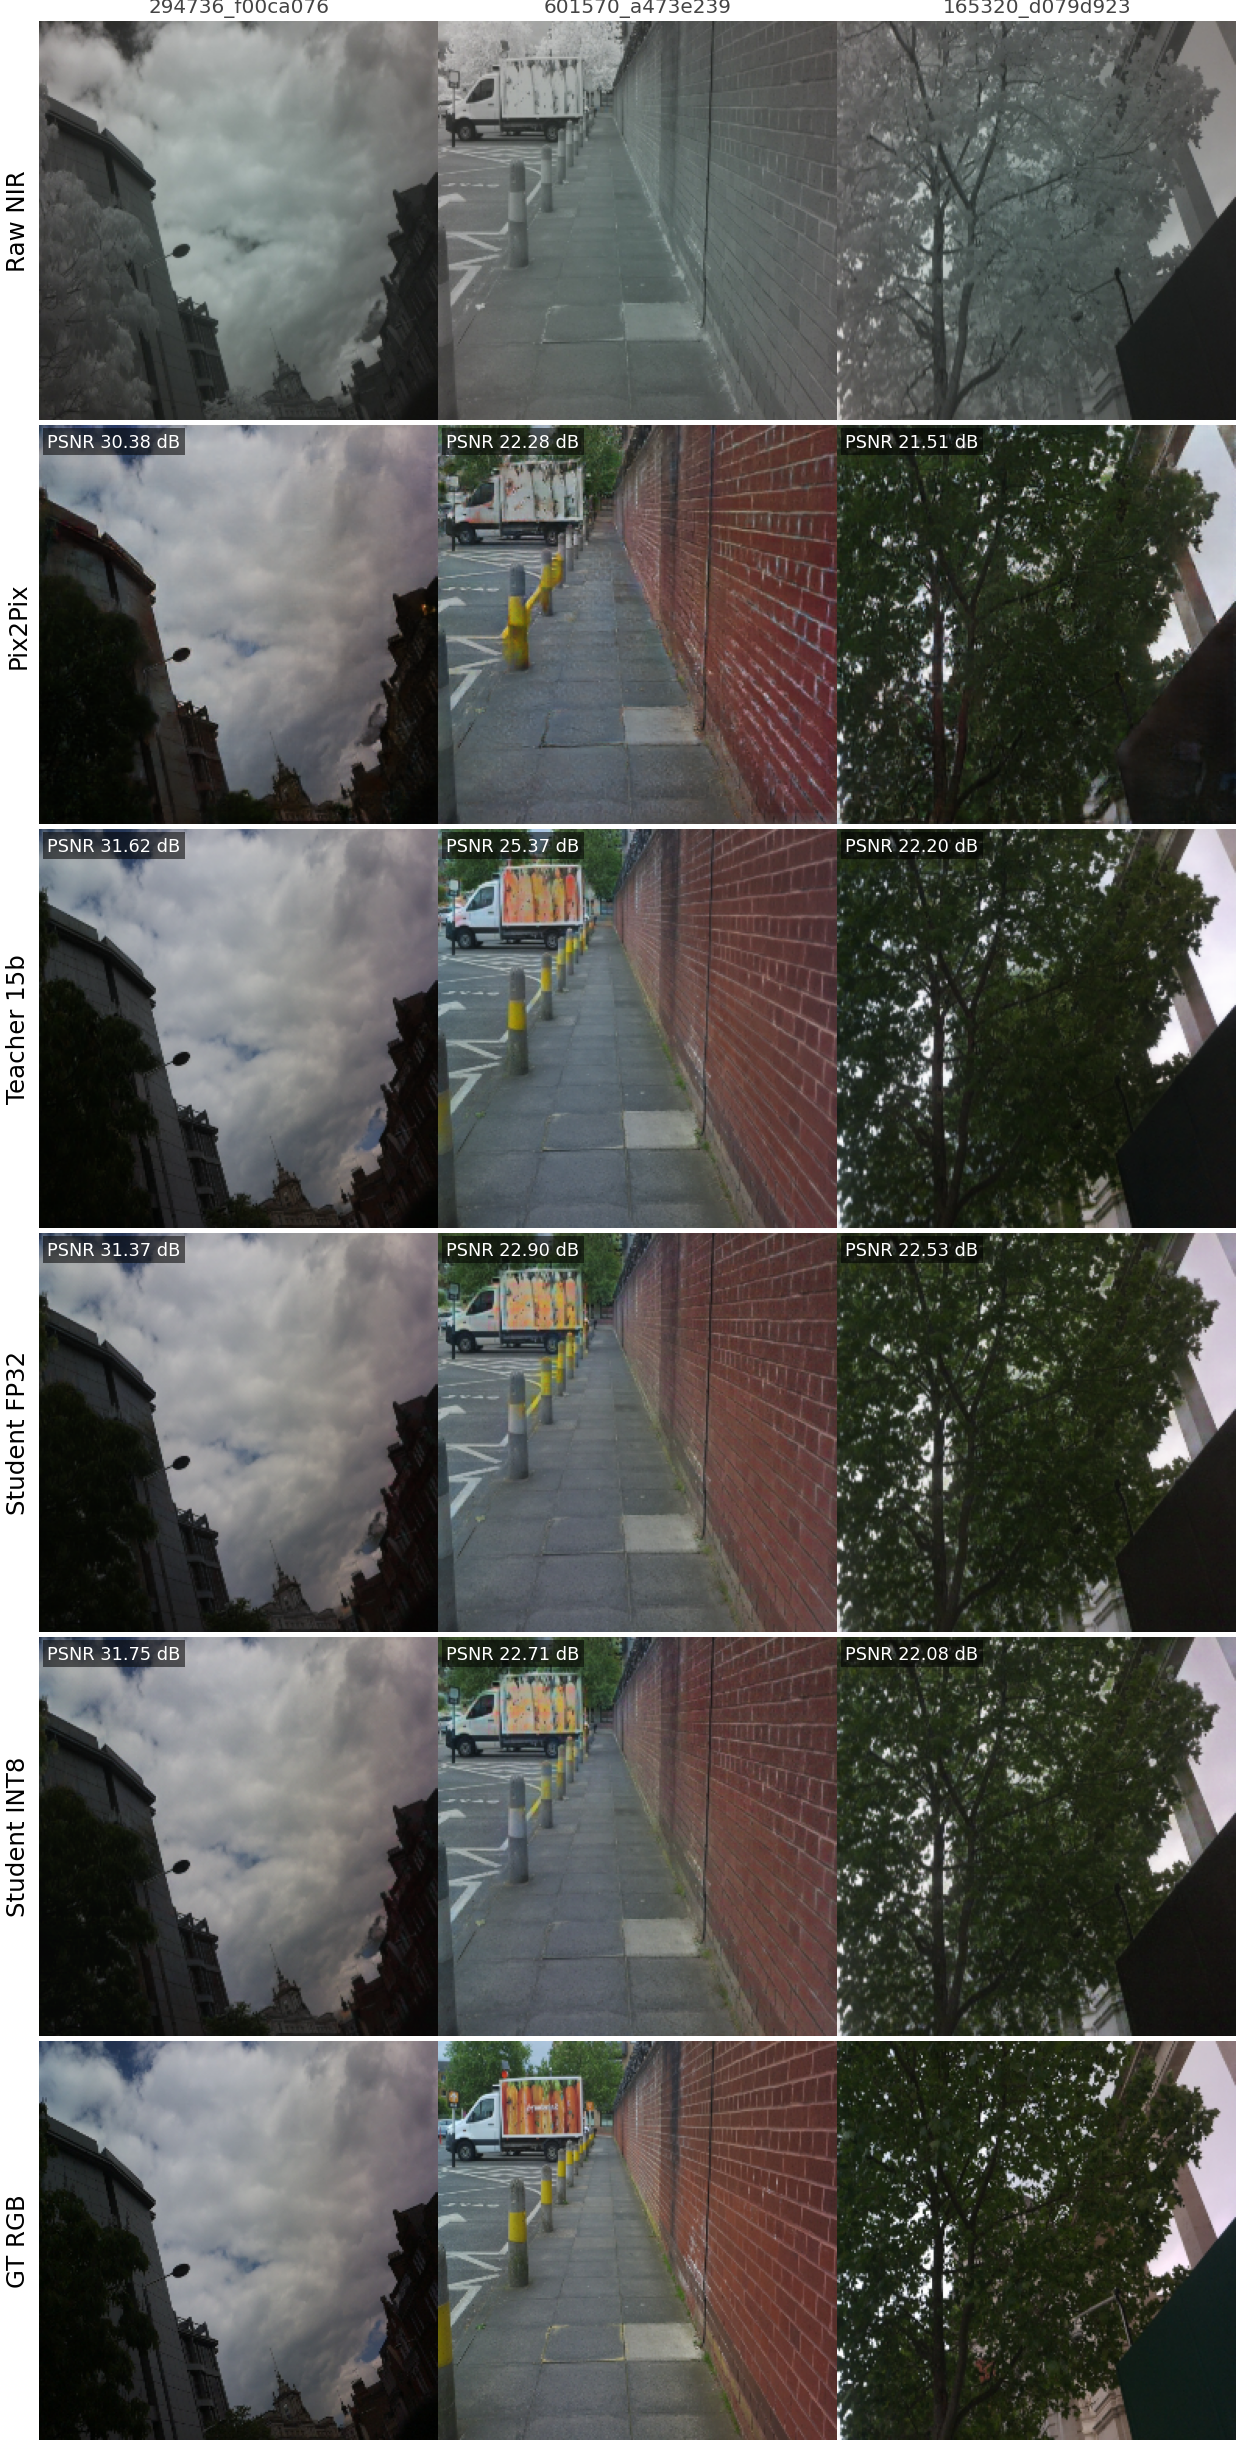
\includegraphics[height=0.9\textheight]{imgs/random_no_people_grid.png}
\caption{Random samples. The rows show, top to bottom: raw NIR, Pix2Pix, teacher, feature-KD student FP32, feature-KD student INT8, and ground-truth RGB. PSNR values are reported for each model.}
\label{fig:student_compare_grid}
\end{figure}

\section{Downstream Agreement}
\label{sec:res_downstream}

The final teacher, FP32 student and deployed mixed-INT8 student are evaluated with a panel of frozen RGB-pretrained models, asking whether translation restores behaviour closer to that observed on native RGB without retraining. The evaluation covers foundation-model embeddings, object detection, semantic segmentation and depth estimation. These are behavioural-agreement measurements against native-RGB model outputs rather than human-labelled task accuracy.

\subsection{Foundation and Independent Embedding Agreement}

\autoref{tab:res_pixel_embedding} measures cosine agreement with native RGB in four representation spaces. DINOv2-S supplied a training loss, and the CLIP evaluator is partially related to training because CLIP-B/32 supplied a loss and checkpoint-selection signal while the test evaluator uses CLIP-B/16. DINOv2-L~\cite{oquab2024dinov2} and SigLIP2~\cite{tschannen2025siglip2} did not appear in the training objective and therefore provide the stronger independent probes. CLIP-FID complements the per-image cosine metrics with a distribution-level comparison over the complete test split.

\begin{table}[!htbp]
\centering
\scriptsize
\setlength{\tabcolsep}{2.5pt}
\resizebox{\linewidth}{!}{%
\begin{tabular}{llcccccc}
\hline
\textbf{Evaluator} & \textbf{Training overlap} & \textbf{Raw NIR} & \textbf{Pix2Pix} & \textbf{Teacher} & \textbf{Student FP32} & \textbf{Student INT8} \\
\hline
\multicolumn{7}{l}{\textbf{Cosine similarity, mean [95\% CI]} $\uparrow$} \\
DINOv2-S & Yes & 0.7273 [0.7185, 0.7361] & 0.8072 [0.8005, 0.8136] & 0.9499 [0.9465, 0.9530] & 0.9228 [0.9188, 0.9266] & 0.9166 [0.9124, 0.9206] \\
DINOv2-L & No & 0.7282 [0.7198, 0.7365] & 0.7229 [0.7153, 0.7304] & 0.9206 [0.9162, 0.9248] & 0.8816 [0.8765, 0.8864] & 0.8709 [0.8654, 0.8761] \\
CLIP-B/16 & Partial & 0.8563 [0.8534, 0.8593] & 0.8774 [0.8739, 0.8809] & 0.9572 [0.9550, 0.9593] & 0.9287 [0.9259, 0.9315] & 0.9202 [0.9173, 0.9230] \\
SigLIP2 base/256 & No & 0.8829 [0.8803, 0.8854] & 0.8940 [0.8909, 0.8971] & 0.9619 [0.9600, 0.9636] & 0.9459 [0.9437, 0.9480] & 0.9427 [0.9404, 0.9449] \\
\hline
\multicolumn{7}{l}{\textbf{Distribution-level distance} $\downarrow$} \\
CLIP-FID & Partial & 17.86 & 11.94 & 2.47 & 5.50 & 6.95 \\
\hline
\end{tabular}
}
\caption{Embedding agreement with native RGB. Cosine rows report per-image means with 95\% image-bootstrap confidence intervals. ``Partial'' shows evaluator-family overlap rather than reuse of the exact test-time weights.}
\label{tab:res_pixel_embedding}
\end{table}

The teacher is strongest on every representation metric, but the students retain substantial improvement over raw NIR. On the independent DINOv2-L probe, cosine similarity rises from 0.7282 for raw NIR to 0.8816 for the FP32 student and 0.8709 after quantisation, corresponding to gap closures of 0.566 and 0.525. On independent SigLIP2, the respective closures are 0.538 and 0.511. The Pix2Pix baseline closes almost none of this representation gap, with closures of -0.020 on DINOv2-L and +0.095 on SigLIP2. The confidence intervals for raw NIR and both student variants are clearly separated on both independent probes.

Quantisation reduces every cosine score slightly, with DINOv2-L falling by 0.0107 and SigLIP2 by 0.0032 relative to the FP32 student. The distribution-level effect is larger, with CLIP-FID increasing from 5.50 to 6.95, a 26.37\% deterioration, although it remains substantially below the raw-NIR value of 17.86. These results support retained representation-level agreement after compression and quantisation, but DINOv2-S and CLIP-family scores are treated as supporting rather than independent evidence because of their relationship to the training objective.

\subsection{Object Detection}

Detection agreement is evaluated with YOLOv8m and RT-DETR-L using COCO-style mAP at IoU 0.5 and over thresholds 0.5:0.95. Native-RGB detections are treated as pseudo-ground truth, so native-RGB self-agreement is 1 by definition.

\begin{table}[!htbp]
\centering
\footnotesize
\begin{tabular}{llccccc}
\hline
\textbf{Detector} & \textbf{Metric} & \textbf{Raw NIR} & \textbf{Pix2Pix} & \textbf{Teacher} & \textbf{Student FP32} & \textbf{Student INT8} \\
\hline
YOLOv8m & mAP@0.5 $\uparrow$ & 0.224 & 0.106 & 0.308 & 0.284 & 0.288 \\
        & mAP@0.5:0.95 $\uparrow$ & 0.187 & 0.081 & 0.259 & 0.242 & 0.246 \\
RT-DETR-L & mAP@0.5 $\uparrow$ & 0.243 & 0.148 & 0.390 & 0.297 & 0.283 \\
          & mAP@0.5:0.95 $\uparrow$ & 0.205 & 0.120 & 0.339 & 0.252 & 0.241 \\
\hline
\end{tabular}
\caption{Object-detection agreement with native-RGB pseudo-labels. Metrics use COCO-style mAP@0.5 and mAP@0.5:0.95. Reference detections come from the same frozen detector on native RGB rather than human annotations.}
\label{tab:res_detection}
\end{table}

The teacher improves both metrics for both detectors and produces the strongest detection agreement overall. Using the primary mAP@0.5 metric, its gap closure is 0.108 for YOLOv8m and 0.194 for RT-DETR-L. Distillation reduces these gains, and the FP32 student's closures are 0.077 and 0.072 respectively. Nevertheless, both remain positive, showing that the selected student moves both detector outputs toward their native-RGB behaviour rather than merely preserving the raw-NIR baseline. Pix2Pix, by contrast, falls below the raw-NIR baseline on both detectors, with mAP@0.5 closures of -0.152 for YOLOv8m and -0.125 for RT-DETR-L.

Quantisation has a detector-dependent effect. YOLOv8m mAP@0.5 rises slightly from 0.284 to 0.288, increasing gap closure from 0.077 to 0.083. RT-DETR-L mAP@0.5 falls from 0.297 to 0.283, reducing closure from 0.072 to 0.053. The same direction is visible in mAP@0.5:0.95. Thus, INT8 retains positive agreement recovery for both independent detectors, but the small YOLO improvement should not be interpreted as a general benefit of quantisation.

\subsection{Semantic Segmentation}
\label{sec:res_seg}

Segmentation is evaluated using Dice agreement with the native-RGB SegFormer prediction on images where the reference class occupies at least 5\% of pixels. ADE20K and Cityscapes are reported separately because their category sets and training distributions differ.

\autoref{tab:res_seg_ade} reports the four ADE20K classes used in the primary summary. \autoref{tab:res_seg_cityscapes} reports the 18 defined Cityscapes classes. Traffic light has no qualifying examples and is excluded from the class-unweighted mean.

\begin{table}[!htbp]
\centering
\scriptsize
\setlength{\tabcolsep}{2.5pt}
\resizebox{\linewidth}{!}{%
\begin{tabular}{lcccccc}
\hline
\textbf{Class} & \textbf{$n$} & \textbf{Raw NIR [95\% CI]} & \textbf{Pix2Pix [95\% CI]} & \textbf{Teacher [95\% CI]} & \textbf{Student FP32 [95\% CI]} & \textbf{Student INT8 [95\% CI]} \\
\hline
Tree & 665 & 0.625 [0.598, 0.651] & 0.897 [0.885, 0.908] & 0.945 [0.938, 0.951] & 0.921 [0.912, 0.930] & 0.917 [0.908, 0.926] \\
Person & 226 & 0.685 [0.643, 0.724] & 0.679 [0.642, 0.714] & 0.856 [0.831, 0.879] & 0.834 [0.810, 0.857] & 0.823 [0.797, 0.847] \\
Building & 869 & 0.797 [0.781, 0.811] & 0.862 [0.851, 0.874] & 0.915 [0.905, 0.924] & 0.894 [0.883, 0.904] & 0.891 [0.879, 0.901] \\
Road & 323 & 0.669 [0.636, 0.701] & 0.762 [0.733, 0.789] & 0.881 [0.864, 0.899] & 0.845 [0.824, 0.865] & 0.842 [0.821, 0.861] \\
\hline
Class-unweighted mean & -- & 0.694 & 0.750 & 0.899 & 0.874 & 0.868 \\
\hline
\end{tabular}
}
\caption{SegFormer-B0-ADE20K Dice agreement with native-RGB pseudo-labels. Rows include only test images where the native-RGB reference class covers at least 5\% of pixels.}
\label{tab:res_seg_ade}
\end{table}

\begin{table}[!htbp]
\centering
\scriptsize
\setlength{\tabcolsep}{2pt}
\resizebox{\linewidth}{!}{%
\begin{tabular}{lcccccc}
\hline
\textbf{Class} & \textbf{$n$} & \textbf{Raw NIR [95\% CI]} & \textbf{Pix2Pix [95\% CI]} & \textbf{Teacher [95\% CI]} & \textbf{Student FP32 [95\% CI]} & \textbf{Student INT8 [95\% CI]} \\
\hline
Road & 680 & 0.653 [0.627, 0.678] & 0.789 [0.770, 0.809] & 0.846 [0.830, 0.861] & 0.811 [0.794, 0.828] & 0.811 [0.793, 0.828] \\
Sidewalk & 321 & 0.528 [0.494, 0.561] & 0.566 [0.533, 0.599] & 0.743 [0.719, 0.767] & 0.661 [0.631, 0.690] & 0.635 [0.603, 0.666] \\
Building & 920 & 0.700 [0.684, 0.716] & 0.805 [0.792, 0.817] & 0.864 [0.852, 0.876] & 0.833 [0.820, 0.846] & 0.822 [0.808, 0.836] \\
Wall & 109 & 0.263 [0.209, 0.316] & 0.407 [0.345, 0.472] & 0.618 [0.560, 0.670] & 0.539 [0.481, 0.594] & 0.525 [0.471, 0.577] \\
Fence & 184 & 0.489 [0.440, 0.538] & 0.500 [0.456, 0.544] & 0.692 [0.651, 0.731] & 0.618 [0.573, 0.660] & 0.609 [0.565, 0.652] \\
Pole & 32 & 0.679 [0.581, 0.766] & 0.627 [0.522, 0.723] & 0.747 [0.636, 0.843] & 0.717 [0.630, 0.790] & 0.632 [0.512, 0.742] \\
Traffic sign & 4 & 0.211 [0.000, 0.610] & 0.159 [0.000, 0.414] & 0.418 [0.064, 0.772] & 0.398 [0.000, 0.796] & 0.410 [0.000, 0.821] \\
Vegetation & 808 & 0.641 [0.618, 0.664] & 0.878 [0.867, 0.887] & 0.934 [0.927, 0.941] & 0.910 [0.901, 0.919] & 0.903 [0.893, 0.911] \\
Terrain & 86 & 0.041 [0.020, 0.066] & 0.864 [0.812, 0.908] & 0.881 [0.833, 0.924] & 0.856 [0.801, 0.903] & 0.857 [0.805, 0.902] \\
Sky & 542 & 0.767 [0.740, 0.792] & 0.921 [0.907, 0.935] & 0.957 [0.947, 0.966] & 0.939 [0.927, 0.951] & 0.920 [0.904, 0.936] \\
Person & 271 & 0.601 [0.563, 0.639] & 0.619 [0.584, 0.653] & 0.775 [0.745, 0.805] & 0.725 [0.691, 0.758] & 0.714 [0.680, 0.748] \\
Rider & 32 & 0.091 [0.023, 0.176] & 0.402 [0.317, 0.488] & 0.702 [0.628, 0.764] & 0.591 [0.500, 0.671] & 0.479 [0.377, 0.577] \\
Car & 191 & 0.683 [0.639, 0.726] & 0.634 [0.587, 0.680] & 0.793 [0.756, 0.828] & 0.726 [0.682, 0.768] & 0.712 [0.667, 0.755] \\
Truck & 31 & 0.296 [0.193, 0.405] & 0.223 [0.127, 0.330] & 0.422 [0.304, 0.543] & 0.351 [0.245, 0.465] & 0.300 [0.190, 0.421] \\
Bus & 16 & 0.334 [0.169, 0.509] & 0.410 [0.268, 0.552] & 0.478 [0.294, 0.662] & 0.401 [0.226, 0.581] & 0.361 [0.183, 0.545] \\
Train & 31 & 0.195 [0.112, 0.284] & 0.115 [0.042, 0.206] & 0.349 [0.245, 0.453] & 0.198 [0.107, 0.301] & 0.163 [0.082, 0.259] \\
Motorcycle & 18 & 0.303 [0.172, 0.452] & 0.482 [0.357, 0.605] & 0.726 [0.620, 0.820] & 0.612 [0.535, 0.695] & 0.641 [0.574, 0.717] \\
Bicycle & 36 & 0.580 [0.472, 0.684] & 0.721 [0.651, 0.786] & 0.716 [0.624, 0.803] & 0.666 [0.572, 0.757] & 0.655 [0.557, 0.751] \\
\hline
Mean excluding traffic light & -- & 0.447 & 0.572 & 0.703 & 0.642 & 0.619 \\
\hline
\end{tabular}
}
\caption{SegFormer-B0-Cityscapes Dice agreement with native-RGB pseudo-labels. Traffic light has no qualifying examples and is excluded from the mean. All reported values include 95\% bootstrap confidence intervals from 10{,}000 image-level resamples.}
\label{tab:res_seg_cityscapes}
\end{table}

Both segmentation tasks show a larger recovery than detection. ADE20K class-mean Dice improves from 0.694 on raw NIR to 0.874 for the FP32 student and 0.868 after INT8 conversion, giving gap closures of 0.587 and 0.569. Cityscapes class-mean Dice improves from 0.447 to 0.642 for FP32 and 0.619 for INT8, giving closures of 0.351 and 0.311. Pix2Pix achieves smaller but positive closures of +0.183 on ADE20K and +0.226 on Cityscapes, making segmentation the one task family where the baseline recovers some native-RGB behaviour. Quantisation slightly reduces both means, with the larger loss on the Cityscapes distribution.

\subsection{Depth}

Depth agreement is evaluated with DepthAnything-Small. The metric is per-image min--max-normalised L1 distance to the native-RGB depth prediction, so lower is better.

\begin{table}[!htbp]
\centering
\footnotesize
\resizebox{\linewidth}{!}{%
\begin{tabular}{llccccc}
\hline
\textbf{Model} & \textbf{Metric} & \textbf{Raw NIR} & \textbf{Pix2Pix} & \textbf{Teacher} & \textbf{Student FP32} & \textbf{Student INT8} \\
\hline
DepthAnything-Small & Normalised L1 $\downarrow$ & 0.677 [0.641, 0.715] & 0.678 [0.642, 0.715] & 0.365 [0.344, 0.387] & 0.424 [0.402, 0.447] & 0.455 [0.429, 0.482] \\
\hline
\end{tabular}
}
\caption{DepthAnything-Small agreement with native-RGB depth predictions. Normalised L1 is computed after per-image min--max normalisation and should not be read as metres.}
\label{tab:res_depth}
\end{table}

The FP32 and INT8 students both improve substantially over raw NIR. Their normalised L1 closures are 0.374 and 0.328 respectively. Pix2Pix's closure is -0.001, so its depth agreement is indistinguishable from raw NIR. Quantisation increases the error by 0.0308 relative to the FP32 student, which is the largest relative quality loss among the five primary tasks.

\subsection{Headline Gap-Closure Summary}
\label{sec:res_gapclosure}

\autoref{tab:res_gapclosure} summarises the primary success criterion. The five primary tasks are the two detection models, the two segmentation distributions and the depth evaluator. Independent embedding probes are shown as supporting evidence because they are useful checks on representation recovery but are not counted as separate primary tasks.

\begin{table}[!htbp]
\centering
\footnotesize
\resizebox{\linewidth}{!}{%
\begin{tabular}{llccccccc}
\hline
\textbf{Task} & \textbf{Primary metric} & \textbf{Raw} & \textbf{Pix2Pix} & \textbf{Pix2Pix closure} & \textbf{Student FP32} & \textbf{FP32 closure} & \textbf{Student INT8} & \textbf{INT8 closure} \\
\hline
Detection 1 & YOLOv8m mAP@0.5 & 0.224 & 0.106 & -0.152 & 0.284 & +0.077 & 0.288 & +0.083 \\
Detection 2 & RT-DETR-L mAP@0.5 & 0.243 & 0.148 & -0.125 & 0.297 & +0.072 & 0.283 & +0.053 \\
Segmentation 1 & ADE class-mean Dice & 0.694 & 0.750 & +0.183 & 0.874 & +0.587 & 0.868 & +0.569 \\
Segmentation 2 & Cityscapes class-mean Dice & 0.447 & 0.572 & +0.226 & 0.642 & +0.351 & 0.619 & +0.311 \\
Depth & Normalised L1 & 0.677 & 0.678 & -0.001 & 0.424 & +0.374 & 0.455 & +0.328 \\
Independent embedding & DINOv2-L cosine & 0.728 & 0.723 & -0.020 & 0.882 & +0.566 & 0.871 & +0.525 \\
Independent embedding & SigLIP2 cosine & 0.883 & 0.894 & +0.095 & 0.946 & +0.538 & 0.943 & +0.511 \\
\hline
\end{tabular}
}
\caption{Headline gap-closure summary for the selected student before and after mixed-INT8 export. Positive closure means the translated output is closer to native-RGB model behaviour than raw NIR. For the lower-is-better depth metric, the closure sign is inverted by the harness. }
\label{tab:res_gapclosure}
\end{table}

Both student precisions pass S2 with positive closure on all five primary tasks, and neither falls below its raw-NIR baseline. Quantisation retains positive closure on all seven reported probes, although it reduces six of the seven closure values. YOLOv8m is the exception and improves slightly.

Pix2Pix is the standard baseline for paired image-to-image translation and the formulation most later methods build on~\cite{isola2017image,wang2018pix2pixhd,park2019spade,pix2next2024}, so it is a fair point of comparison. It is also the sharpest illustration of why downstream agreement, not pixel fidelity, is the right success criterion. It ties the student on pixel and structural fidelity, yet on the independent DINOv2-L probe it sits at 0.723, indistinguishable from the 0.728 of doing no translation at all, and on depth its 0.678 equals raw NIR exactly. The student reaches 0.882 and 0.424 on the same probes. On detection Pix2Pix is worse than the untranslated input, falling from raw NIR's 0.224 to 0.106 mAP@0.5 on YOLOv8m and from 0.243 to 0.148 on RT-DETR-L, closures of -0.152 and -0.125, where both student precisions stay positive. A baseline that looks competitive on classic metrics therefore contributes almost nothing to the downstream behaviour the translator is meant to restore. It is also a 54.4\,M-parameter model against the student's 1.7\,M, so unlike the student it is not a candidate for the Raspberry~Pi.

\section{Teacher Ablation Study}
\label{sec:res_ablation}

\subsection{Ablation Results}

\autoref{tab:abl_summary} reports ablation evidence for the teacher recipe. All NAFNet variants outperform Pix2Pix on PSNR, LPIPS, DINOv2-L, ADE Dice and depth L1. Removing the foundation-feature ensemble (No FM) improves pixel fidelity but markedly reduces downstream agreement metrics, indicating that the feature-matching term is essential to the downstream gains. The other ablations (No GAN, No MS-SSIM, No FM warm-up) sit within confidence intervals on DINOv2-L and depth, suggesting these components are not individually critical on those probes. The adversarial term nevertheless earns its place on detection: removing it drops YOLO closure from +0.108 to +0.077, the largest detection change among these ablations, and at weight 0.3 it adds little training cost or instability. The final teacher therefore retains the full objective and represents the clean baseline for deployment.

\begin{table}[!htbp]
\centering
\scriptsize
\setlength{\tabcolsep}{2pt}
\resizebox{\linewidth}{!}{%
\begin{tabular}{lp{0.24\linewidth}cccccc}
\hline
\textbf{Configuration} & \textbf{Exact change} & \textbf{PSNR} & \textbf{LPIPS} & \textbf{DINOv2-L} & \textbf{YOLO closure} & \textbf{ADE closure} & \textbf{Depth L1} \\
\hline
Raw NIR & no translation & 16.65 & 0.337 & 0.728 & 0.000 & 0.000 & 0.677 \\
Pix2Pix & U-Net baseline & 24.03 & 0.185 & 0.723 & -0.152 & 0.183 & 0.678 \\
No FM & FM weights zero & 27.10 & 0.098 & 0.886 & +0.011 & 0.619 & 0.420 \\
No GAN & GAN disabled & 26.33 & 0.100 & 0.923 & +0.077 & 0.667 & 0.347 \\
No MS-SSIM & MS-SSIM disabled & 26.29 & 0.102 & 0.922 & +0.076 & 0.653 & 0.348 \\
No FM warm-up& FM active without warm-up & 26.31 & 0.101 & 0.921 & +0.064 & 0.665 & 0.353 \\
Final teacher & full objective & 26.16 & 0.103 & 0.921 & +0.108 & 0.670 & 0.365 \\
\hline
\end{tabular}
}
\caption{Teacher ablation summary on the canonical held-out test split.}
\label{tab:abl_summary}
\end{table}



\subsection{Pixel-side versus feature-side changes}
\label{sec:res_abl_lossfixes}

Two intermediate objective changes preceded the final ensemble. The first targeted the pixel side, using an NIR-gradient-weighted L1 that downweights the loss in flat NIR regions, on the reasoning that colour is poorly determined there and penalising those regions equally pushes the model toward desaturated, average colour. In practice this made almost no difference, and if anything cost a small amount of performance, indicating that the baseline's weakness was not a mis-weighted pixel term. The change that mattered was on the feature side, adding a \emph{task-facing feature loss} in which the generated and real RGB are passed through frozen RGB-trained models and the differences in their early and mid activations are penalised. This directly optimises agreement in the representations the downstream panel uses, rather than pixel colour or a generic VGG perceptual space. The first feature-supervised NAFNet used ResNet-50 and SegFormer features, providing the proof of concept that led to the foundation-model ensemble of the final teacher.

\begin{figure}[!htbp]
\centering
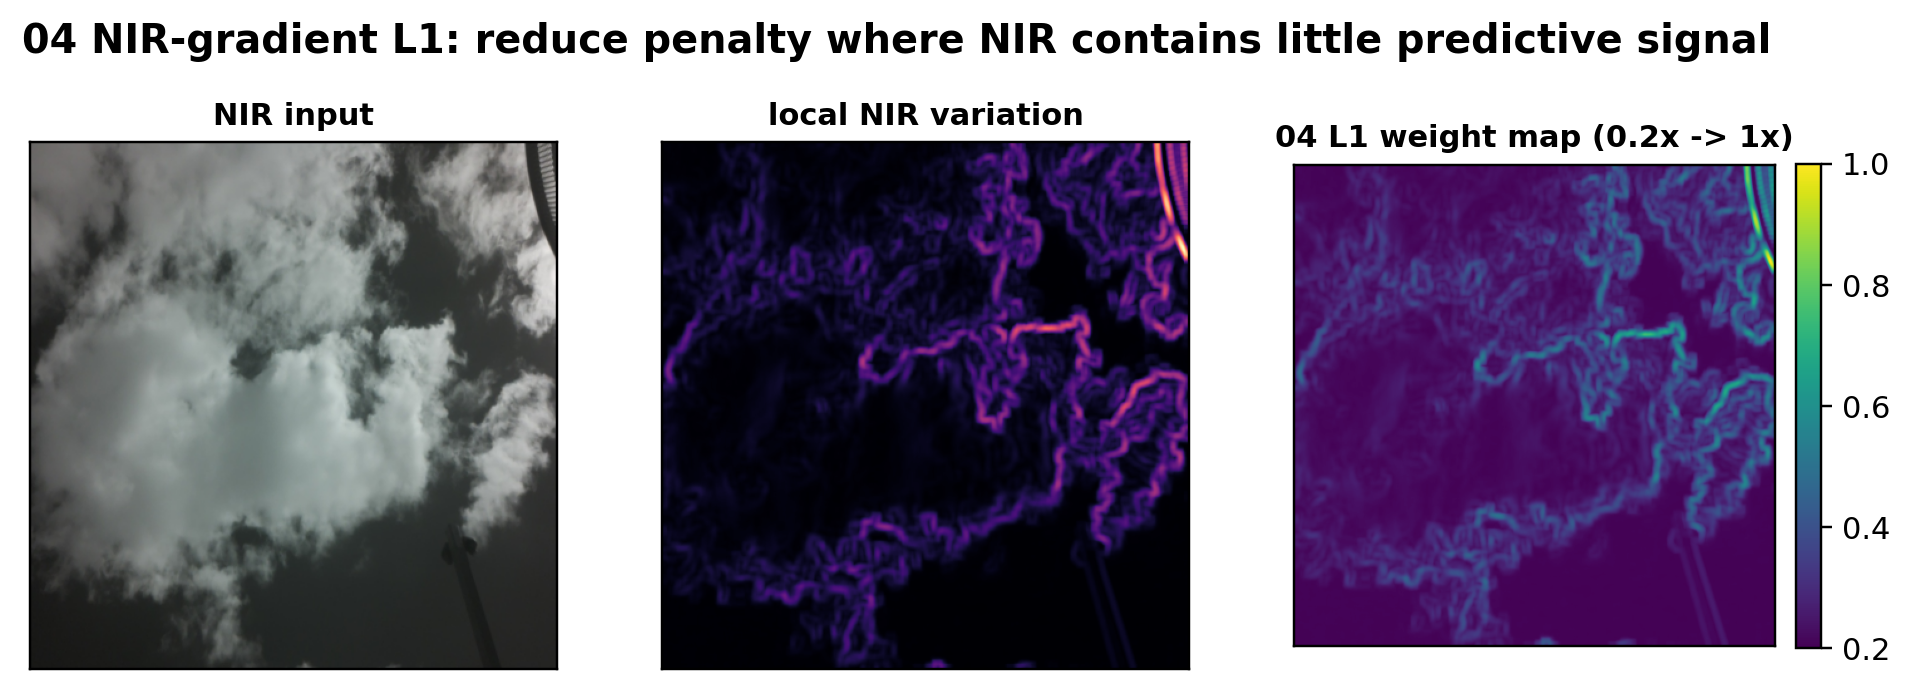
\includegraphics[width=\linewidth]{imgs/ablations/nir_gradient_l1.png}
\caption{NIR-gradient-weighted L1. From the NIR input (left), local NIR variation (centre) drives a per-pixel L1 weight map (right) that scales the penalty from $0.2\times$ in flat, low-signal regions to $1\times$ at strong NIR edges. In practice this reweighting made almost no difference to downstream agreement, indicating the baseline's weakness was not a mis-weighted pixel term.}
\label{fig:nir_gradient_l1}
\end{figure}

\section{Student Distillation Ablations}
\label{sec:res_student_ablation}

The teacher ablations above choose the high-capacity teacher. A separate question is how to compress it into the width-16 student without losing the downstream behaviour that made the teacher useful. These are not different student architectures: each variant uses the same NAFNet-16 backbone and the same teacher-output L1 distillation term. What changes is the auxiliary supervision used to teach the small model what matters.

\begin{description}
    \item[Baseline KD.] This is the minimum task-facing student. It distils the teacher output with an L1 term and adds DINOv2 and CLIP feature losses against the RGB ground truth. It tests whether the compact student can recover the teacher's broad semantic alignment using only generic foundation-feature supervision.
    \item[Downstream heads.] This keeps the same student architecture but broadens the feature losses to include ResNet-50, SegFormer and DepthAnything. It tests whether adding classifier, segmentation and depth representations preserves the downstream behaviours measured by the evaluation harness, rather than only matching generic image embeddings.
    \item[Feature KD.] This adds feature-level knowledge distillation from the teacher: frozen-feature activations are matched between the student's output and the teacher's output, not only between the student's output and RGB ground truth. It tests whether the student should imitate the teacher's representation-space behaviour directly when the teacher's output is the deployed target.
\end{description}

\autoref{tab:student_distill_ablation} compares these student-training variants.

\begin{table}[!htbp]
\centering
\footnotesize
\setlength{\tabcolsep}{3pt}
\resizebox{\linewidth}{!}{%
\begin{tabular}{lp{0.28\linewidth}cccccccc}
\hline
\textbf{Student variant} & \textbf{Additional signal} & \textbf{PSNR} & \textbf{LPIPS} & \textbf{CLIP-B/16} & \textbf{DINOv2-L} & \textbf{ADE mean} & \textbf{City mean} & \textbf{YOLO} & \textbf{RT-DETR} \\
\hline
Baseline KD & DINOv2 and CLIP to RGB GT & 24.08 & 0.152 & 0.923 & 0.875 & 0.863 & 0.631 & 0.264 & 0.296 \\
Downstream heads & DINOv2, CLIP, ResNet-50, SegFormer and DepthAnything & 23.59 & 0.155 & 0.917 & 0.867 & 0.860 & 0.624 & 0.220 & 0.302 \\
Feature KD & downstream heads plus feature match to teacher output & \textbf{24.09} & \textbf{0.146} & \textbf{0.929} & \textbf{0.882} & \textbf{0.874} & \textbf{0.642} & \textbf{0.284} & 0.297 \\
\hline
\end{tabular}
}
\caption{Student distillation ablation for the width-16 NAFNet. All variants use 1.7\,M parameters and the same backbone, and only the auxiliary supervision differs. YOLO and RT-DETR columns report mAP@0.5 agreement.}
\label{tab:student_distill_ablation}
\end{table}

The feature-KD student is selected by the predeclared highest validation CLIP-cosine rule and is also strongest on most of the quality and downstream probes. It compresses the 116\,M teacher parameters to 1.7\,M, a $67.3\times$ reduction, while losing 2.07\,dB PSNR and 0.039 DINOv2-L cosine relative to the teacher.

\section{Generalisation to Other Modalities}
\label{sec:res_modality_extension}

The foundation-model feature-matching recipe is not specific to NIR, so it was also tested on thermal and SAR imagery to find where it stops working.

On thermal imagery (KAIST), which shares no spectral overlap with the visible band, the recipe transfers without modification. CLIP cosine similarity reaches 0.924 compared to 0.46 on raw thermal, and static scene classes improve in downstream segmentation (roads +0.3 Dice, vegetation +0.7 Dice, sky +0.8 Dice). The person class fails, because raw thermal's strong pedestrian contrast (people are warm) is lost when the model spends capacity on global colour synthesis. The same weakness appears in the NIR results.

\begin{figure}[!htbp]
\centering
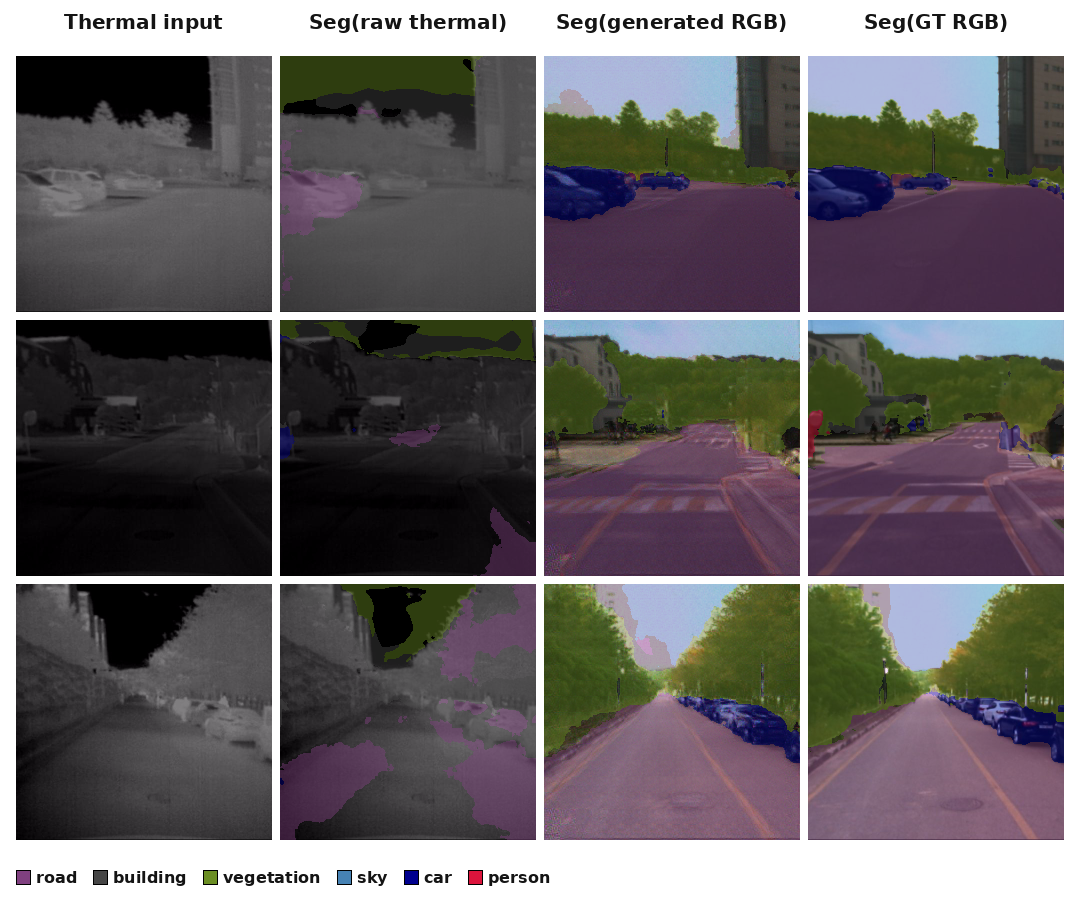
\includegraphics[width=0.90\linewidth]{imgs/seg_kaist.png}
\caption{Downstream segmentation improvement on KAIST thermal. Structures like roads, vegetation and buildings become detectable in the translated output where raw thermal leaves them invisible to standard segmentation models.}
\label{fig:kaist_seg}
\end{figure}

SAR (WHU-SAR-VV, paired SAR/optical patches derived from the WHU-OPT-SAR dataset~\cite{li2022whuoptsar}) is where the approach breaks down. Pixel metrics collapse (PSNR 13.3, SSIM 0.121) and the model plateaus early, while downstream gains are marginal, with EuroSAT~\cite{helber2019eurosat} classification improving from 0.165 to 0.425 and RemoteCLIP~\cite{liu2024remoteclip} cosine reaching 0.759. The recipe helps rare classes (tree Dice improves 10$\times$ from near-invisibility) but absolute performance remains low. The plateau suggests that speckle-aware losses, SAR-specific pretraining or dedicated SAR encoders would be needed to close the gap further.

\section{Edge Performance}
\label{sec:res_edge}
\label{sec:pi_deployment}

For deployment the 116\,M-parameter teacher is distilled into the compact width-16 student selected in Section~\ref{sec:res_student_ablation}. The student was benchmarked on the Raspberry~Pi~5, on the CPU through LiteRT with XNNPACK and ONNX Runtime, and on the Hailo-8L NPU on the Pi AI HAT+. The device ran Raspberry Pi OS on kernel 6.12.75 with HailoRT and Hailo firmware 4.23.0. CPU testing used 100 real test images at $256\times256$ and batch size one, with 10 warmup iterations followed by 100 measurement runs on the default 4-thread configuration. All CPU figures are model-inference latency, the runtime's invoke call on an already prepared input tensor, excluding image decode and pre- and post-processing, while NPU figures are Hailo-8L hardware latency. \autoref{tab:res_edge} reports the results, together with the larger width-32 student variant (11.6\,M parameters, configuration in \autoref{tab:student_arch}) that was also compiled for the NPU.

\begin{table}[!htbp]
\centering
\footnotesize
\begin{tabular}{llccc}
\hline
\textbf{Backend} & \textbf{Model} & \textbf{Latency (ms)} & \textbf{FPS} & \textbf{Artefact} \\
\hline
Hailo-8L NPU & Width-16 student & 36.3 & 27.2 & 17.7\,MB HEF \\
Hailo-8L NPU & Width-32 student & 91.5 & 10.8 & 50.4\,MB HEF \\
CPU LiteRT INT8 & Width-16 student & 198.0 & 5.05 & 2.3\,MB \\
CPU LiteRT FP32 & Width-16 student & 227.2 & 4.40 & 7.1\,MB \\
CPU LiteRT INT8 & Width-32 student & 517.0 & 1.93 & 13.0\,MB \\
CPU ONNX FP32 & Width-16 student & 225.2 & 4.44 & 7.6\,MB \\
CPU ONNX INT8 & Width-16 student & 372.8 & 2.68 & 2.5\,MB \\
\hline
\end{tabular}
\caption{Raspberry~Pi~5 benchmark. CPU rows are model-inference latency at four threads (LiteRT through XNNPACK; ONNX rows from a separate session on the same device, input size and thread configuration), and NPU rows are Hailo-8L hardware latency. The width-16 LiteRT mixed-INT8 student is the selected deployment model; it meets the 5\,FPS target on the CPU and clears it with a wide margin on the NPU.}
\label{tab:res_edge}
\end{table}

\paragraph{Throughput and latency.}
On the CPU, only the mixed-INT8 LiteRT student meets the 5\,FPS target, at 5.05\,FPS (p95: 221.2\,ms) against the FP32 student's 4.40\,FPS (p95: 242.1\,ms). The 15\% throughput gain from quantisation runs contrary to the expectation that compressed models trade latency for size. It reflects the narrower operator set of INT8 kernels and the reduced memory bandwidth required, and it makes the INT8 export not merely smaller but necessary to reach the target at all. The margin is nevertheless slim. INT8 latency varied between 180.1 and 252.5\,ms across the 100 timed runs, consistent with normal scheduler and frequency-governor variation under sustained four-thread load, so the mean meets the 200\,ms budget but the 95th percentile does not, and the CPU path should be regarded as marginal against N1. The Hailo NPU removes this concern, running the same student at 27.2\,FPS, a $5.4\times$ speed-up, and lifting the width-32 student from 1.9\,FPS on the CPU to 10.8\,FPS.

\paragraph{LiteRT vs ONNX.}
The ONNX FP32 export is comparable to LiteRT in size and latency (\autoref{tab:res_edge}), but the quantised path is decisive. ONNX INT8 runs at 2.68\,FPS, far short of the target even allowing for session-to-session variation, where LiteRT INT8 reaches 5.05\,FPS. LiteRT is therefore the deployment runtime, with the ONNX exports retained only for cross-platform portability.

\paragraph{Memory footprint.}
The mixed-INT8 artefact is 2.3\,MB against 7.1\,MB for FP32, a $3.1\times$ reduction coming almost entirely from weight quantisation. Peak memory during sustained inference was under 50\,MB, dominated by input/output buffers and the activation cache rather than model parameters, against 7.6\,GB of RAM available on the idle device, and swap (2.0\,GB configured) was never touched.

\paragraph{Sustained operation and thermal behaviour.}
Sustained operation was checked with a sixty-second continuous NPU run of the selected student. Throughput held at 27.3\,FPS across the full run with no degradation, the Pi temperature rose from 59.8 to 64.8\,\textdegree C, and the throttle status stayed clear for every one-second sample, so there was no under-voltage or frequency cap. On-chip Hailo power telemetry is not exposed on the Pi AI HAT+, so power is reported through the Pi-level thermal evidence rather than a board sensor.

\paragraph{Requirement decisions.}
Both N1 and N2 are met. The selected student clears the 5\,FPS throughput target on both the CPU and the NPU, and the 2.3\,MB artefact and sub-50\,MB peak memory run without swap, out-of-memory failure or thermal throttling, so the edge-deployment objective is verified on the target device. Because the CPU margin is slim, with the p95 latency above the 200\,ms budget, the Hailo-8L path is the recommended backend where headroom for pre-processing or tighter tail latency is required.

\subsection{Live demonstration}
\label{sec:res_live_demo}

A real-time web application runs the full pipeline on the Pi and serves it over the network (\autoref{fig:webapp_live}). It captures NIR frames from the rig camera, translates them with the student, and segments the NIR input, the generated RGB and a live RGB reference from a second camera with a frozen SegFormer-B0 Cityscapes model, displaying all three side by side. The translator backend is switchable at runtime between the two Hailo HEFs and four CPU LiteRT profiles, which lets the CPU and NPU paths be compared live. The image-quality numbers are computed against the second camera under a single global homography, which is not pixel-perfect, and are live single-frame measurements that vary with the scene, so they are indicative rather than comparable to the controlled held-out figures of \autoref{tab:res_imagequality}. The demonstration is qualitative evidence that the translator and a downstream segmentation model run together in real time on the device.

\begin{figure}[H]
\centering
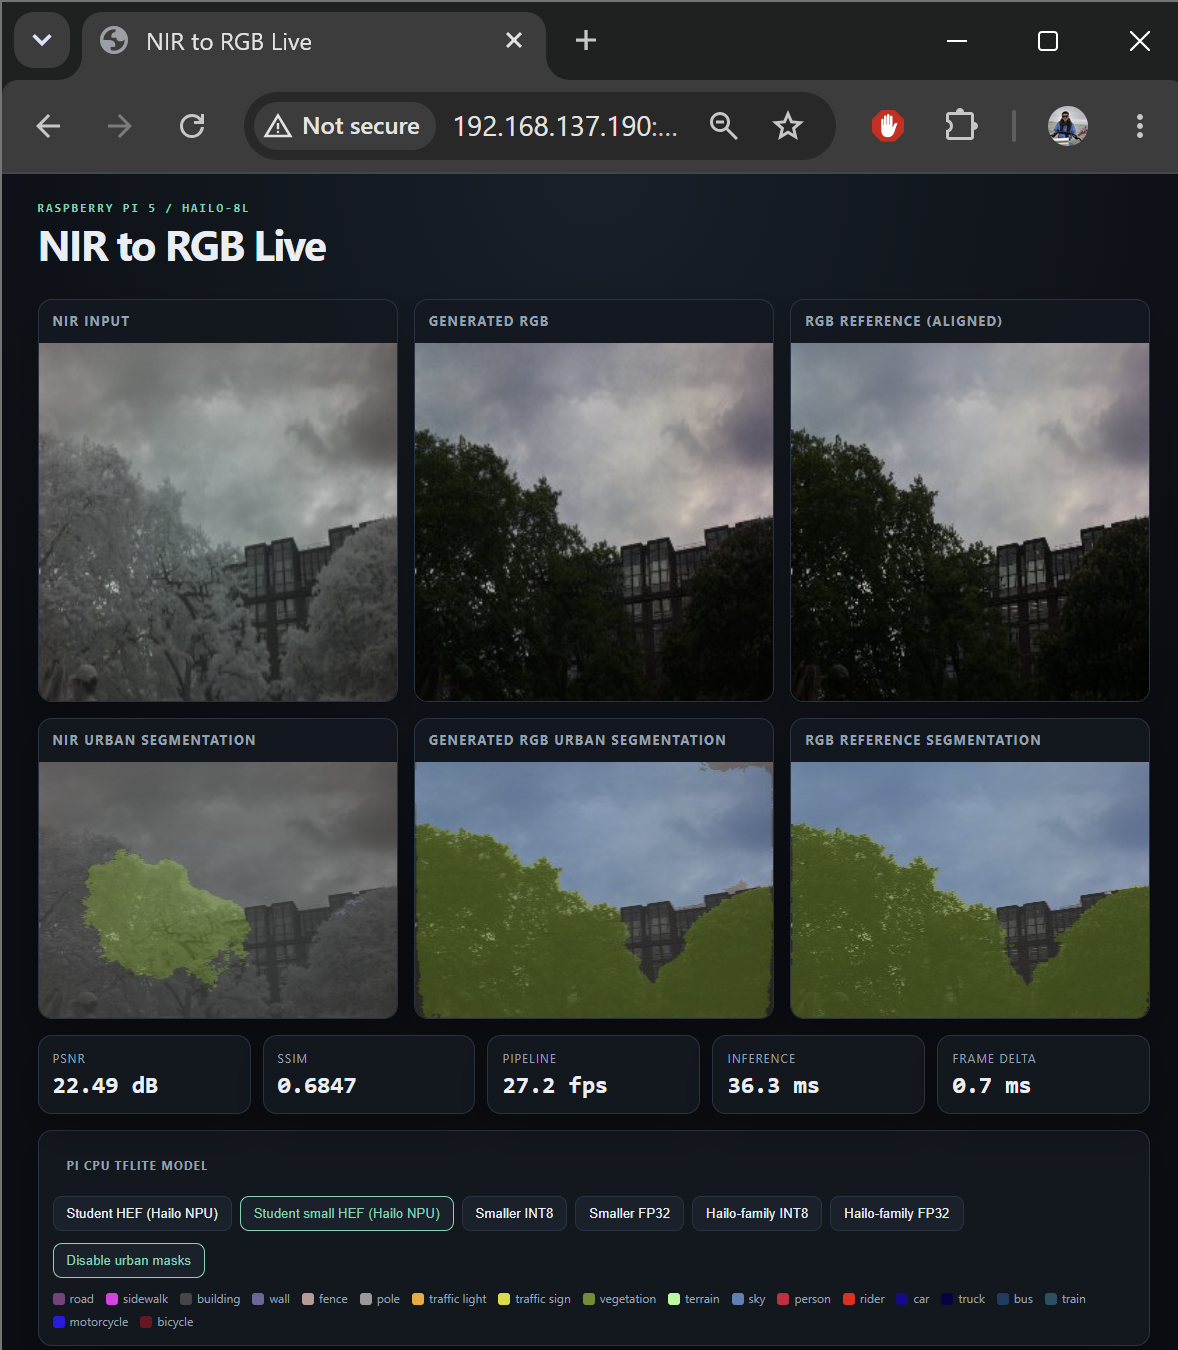
\includegraphics[width=\textwidth]{imgs/webapp_live_demo.png}
\caption{Live on-device web app demonstration on the Raspberry~Pi~5.}
\label{fig:webapp_live}
\end{figure}

\section{Robustness}
\label{sec:res_robustness}

The controlled robustness protocol of Section~\ref{sec:test_robustness} applies deterministic perturbations to the NIR input only, using the first 200 images of the canonical seed-42 test split without further shuffling. \autoref{tab:res_robustness} reports the paired change in each metric relative to the same model's unperturbed run on the same subset, for the final teacher and the selected FP32 student. 

\begin{table}[!htbp]
\centering
\scriptsize
\setlength{\tabcolsep}{3pt}
\resizebox{\linewidth}{!}{%
\begin{tabular}{llcccccccc}
\hline
 & & \multicolumn{4}{c}{\textbf{Teacher}} & \multicolumn{4}{c}{\textbf{Student FP32}} \\
\textbf{Perturbation} & \textbf{Level} & \textbf{$\Delta$PSNR (dB)} & \textbf{$\Delta$LPIPS} & \textbf{$\Delta$CLIP-B/16} & \textbf{$\Delta$DINOv2-L} & \textbf{$\Delta$PSNR (dB)} & \textbf{$\Delta$LPIPS} & \textbf{$\Delta$CLIP-B/16} & \textbf{$\Delta$DINOv2-L} \\
\hline
Exposure gain & 0.8 & -0.57 & +0.006 & -0.001 & -0.002 & -0.73 & +0.007 & -0.003 & -0.002 \\
Exposure gain & 1.2 & -0.74 & +0.002 & -0.002 & -0.003 & -1.14 & +0.005 & -0.002 & -0.005 \\
Gamma & 0.8 & -0.04 & +0.001 & 0.000 & 0.000 & -0.10 & +0.001 & 0.000 & 0.000 \\
Gamma & 1.2 & +0.01 & 0.000 & +0.001 & -0.001 & +0.01 & +0.001 & -0.001 & -0.002 \\
Gaussian blur & $\sigma=1$ & -3.07 & +0.209 & -0.042 & -0.079 & -3.61 & +0.239 & -0.050 & -0.113 \\
Gaussian blur & $\sigma=2$ & -8.47 & +0.509 & -0.179 & -0.367 & -6.75 & +0.499 & -0.144 & -0.300 \\
Gaussian noise & $\sigma=0.01$ & -0.73 & +0.026 & -0.017 & -0.022 & -1.37 & +0.045 & -0.015 & -0.038 \\
Gaussian noise & $\sigma=0.03$ & -5.66 & +0.208 & -0.085 & -0.159 & -5.58 & +0.236 & -0.095 & -0.154 \\
\hline
\end{tabular}
}
\caption{Robustness sweep on the first 200 images of the canonical test split. Each cell is the paired change relative to the same model's clean run on the same subset. Negative $\Delta$PSNR and $\Delta$cosine and positive $\Delta$LPIPS are degradations. Perturbations are applied to the NIR input only. Raw results are in \texttt{experiments/robustness\_v1/per\_image.csv}.}
\label{tab:res_robustness}
\end{table}

Exposure and gamma variation in the tested range is handled well, with the worst case across both models a 1.14\,dB PSNR loss and every embedding change at most 0.005 cosine. Blur and noise define the boundary of the operating envelope. At $\sigma=1$ blur and $\sigma=0.01$ noise the degradation is measurable but moderate, while at $\sigma=2$ blur the teacher loses 8.47\,dB PSNR and 0.367 DINOv2-L cosine and the student loses 6.75\,dB and 0.300, with noise at $\sigma=0.03$ close behind. At that blur level the perturbed outputs sit at DINOv2-L cosines near 0.55--0.57, below the raw-NIR full-test level of 0.728, so outside the envelope the translation no longer offers an embedding-agreement advantage over the untranslated input. These tests are diagnostic rather than a separate success criterion, supporting deployment where input sharpness and noise can be monitored and degraded frames rejected, not unconditional acceptance of arbitrary field conditions.

\section{Key Findings}
\label{sec:res_summary}

The results across this chapter support five main conclusions.

\begin{enumerate}
    \item \textbf{Downstream agreement, not pixel fidelity, is the criterion that matters.} Pix2Pix matches the student on PSNR and SSIM yet recovers almost none of the downstream behaviour, sitting at raw-NIR level on the independent DINOv2-L and depth probes. Pixel metrics alone would have ranked it as competitive and missed this.
    \item \textbf{The foundation-feature teacher closes most of the gap}, moving detection, segmentation, depth and independent embeddings substantially toward native-RGB behaviour, and the No-FM ablation confirms the feature ensemble drives these gains.
    \item \textbf{Distillation preserves that behaviour at a fraction of the size.} The 1.7\,M student keeps positive closure on all five primary tasks, a $67.3\times$ reduction from the teacher, and mixed-INT8 quantisation keeps every closure positive.
    \item \textbf{The student is the only edge-deployable model in the comparison}, meeting the 5\,FPS target on the Pi CPU and reaching 27.2\,FPS on the Hailo-8L NPU with no thermal throttling, while Pix2Pix at 54.4\,M parameters is far too large to run interactively on the device.
    \item \textbf{The recipe generalises only where there is spectral structure}, transferring to thermal but breaking down on SAR, which marks the boundary of the approach.
\end{enumerate}
 % Results
\doublespacing % Do not change - required

\chapter{Critical Evaluation}
\label{ch:evaluation}

%%%%%%%%%%%%%%%%%%%%%%%%%%%%%%%%%%%%%%%
% IMPORTANT
\begin{spacing}{1} %THESE FOUR
\minitoc % LINES MUST APPEAR IN
\end{spacing} % EVERY
\thesisspacing % CHAPTER
% COPY THEM IN ANY NEW CHAPTER
%%%%%%%%%%%%%%%%%%%%%%%%%%%%%%%%%%%%%%%


\section{Achievement of Objectives}
\label{sec:eval_objectives}

The project met its modelling objective. The final assessment is summarised in \autoref{tab:eval_requirements}. All quality and downstream figures are computed over the full 1{,}255-pair held-out test split.

\paragraph{Paired dataset.}
The dataset objective was met in full. The final integrity audit found no missing counterparts, unreadable files, channel mismatches or duplicate image hashes, and the scale proved sufficient to train the teacher and distil the student without exhausting the data.

\paragraph{Translator quality and downstream recovery.}
The final NAFNet teacher improves on both raw NIR and the controlled Pix2Pix baseline on every fidelity metric, and both the FP32 and INT8 students produce positive gap closure on all five primary tasks and on the independent DINOv2-L and SigLIP2 embedding probes. This satisfies S2 in full, where the pre-specified threshold required only three of the five tasks. It does \emph{not} establish absolute detection or segmentation accuracy, since the reference outputs are predictions from the same frozen models on native RGB rather than human annotations. The recovery is also uneven. The detection closures (+0.077 and +0.072 at mAP@0.5) are several times smaller than the segmentation and depth closures (+0.351 to +0.587), making the detectors the weakest primary results. A plausible cause is that detection depends on small objects and fine texture, which translation reproduces least faithfully, whereas segmentation and depth lean on the large-scale structure the translator preserves well.

\paragraph{Edge deployment.}
The distillation, export and quantisation path produced a deployable artefact whose numerical equivalence, determinism and test-set quality were verified off-device, and on-device validation confirms the throughput, memory and thermal requirements (Section~\ref{sec:pi_deployment}). The CPU pass is marginal, however. The mean latency meets the 200\,ms budget but the 95th percentile does not, so real-time CPU deployment has no headroom and the NPU path is the recommended backend.

\begin{table}[!htbp]
\centering
\footnotesize
\resizebox{\linewidth}{!}{%
\begin{tabular}{p{0.08\linewidth}p{0.27\linewidth}p{0.49\linewidth}p{0.08\linewidth}}
\hline
\textbf{Req.} & \textbf{Acceptance condition} & \textbf{Final evidence} & \textbf{Status} \\
\hline
F1 & Same-size three-channel RGB output & Valid $256\times256$ RGB output for all 1{,}255 test inputs & Pass \\
F2 & Geometry preserved & Homography-aligned pairing audited and object boundaries unchanged in translated output & Pass \\
F3 & Deterministic output & Zero mismatched 8-bit pixels over repeated tests of PyTorch, ONNX and LiteRT artefacts & Pass \\
F4 & Drop-in RGB interface & Frozen RGB models accepted translated output without retraining & Pass \\
N1 & At least 5\,FPS model-inference throughput on the Pi~5 & 5.05\,FPS mean on the CPU (mixed-INT8 LiteRT; p95 latency above the 200\,ms budget) and 27.2\,FPS on the Hailo-8L NPU & Pass (marginal on CPU) \\
N2 & Loads and runs within device memory without swapping & 2.3\,MB artefact, peak inference memory under 50\,MB, zero swap observed & Pass \\
S1 & Paired, aligned dataset at sufficient scale & 12{,}536 homography-aligned pairs collected and integrity-audited & Pass \\
S2 & Positive closure on at least three of five behavioural tasks, with no task below its raw-NIR baseline & Positive closure on all five tasks for both FP32 and INT8 students; no task below raw NIR & Pass \\
S3 & Deployed student meets the 5\,FPS target on the Pi~5 & Verified on-device on both the CPU and NPU backends & Pass \\
\hline
\end{tabular}
}
\caption{Assessment of functional and core objectives. F denotes functional requirements, N non-functional requirements, and S success criteria for the main modelling objective.}
\label{tab:eval_requirements}
\end{table}

\section{Comparison with Existing Approaches}
\label{sec:eval_priorwork}

The strongest controlled comparison is the internal Pix2Pix baseline, which uses the same paired data, canonical test split, input resolution and evaluation panel as the final teacher, and its outcome is assessed in Section~\ref{sec:eval_designbets}. Two qualifications apply. First, the baseline received substantially less tuning effort than the final teacher. It is a single run of the standard recipe rather than the product of an ablation campaign, so its result should be read as what the conventional formulation achieves out of the box rather than as the ceiling of GAN-based methods. Second, the NAFNet ablations are single training runs each, and the reported confidence intervals capture per-image variation on the test split, not seed-to-seed training variance, so the component-level conclusions are exploratory, not confirmatory.

Direct numerical comparison with published NIR-to-RGB methods would be misleading. Existing work uses different sensors, spectral cut-offs, scene distributions, alignment quality and evaluation protocols, so the report compares design principles and deployment constraints in Chapter~\ref{ch:background} rather than presenting cross-dataset raw scores as if they were controlled benchmarks.

Fine-tuning each downstream network on NIR would be another plausible alternative, but it was outside the project scope and was not evaluated. The demonstrated advantage of the translator is thus its compatibility with unchanged RGB models; superiority to a fully labelled, task-specific NIR retraining pipeline has not been shown.

\section{Assessment of Design Decisions}
\label{sec:eval_designbets}

\paragraph{Shared-aperture capture rig.}
The rig enabled collection of a much larger project-specific paired dataset than the public datasets considered in Section~\ref{sec:datasets}, and the optical design removes the principal source of depth-dependent parallax.

\paragraph{NAFNet over Pix2Pix.}
This is the decision the evidence supports most directly. The GAN baseline equals the student on PSNR and SSIM yet leaves downstream behaviour near its raw-NIR level (Section~\ref{sec:res_gapclosure}), while the NAFNet path closes most of that gap. The teacher is larger than Pix2Pix, but it is a training-time model only, and after distillation the deployed student is roughly $32\times$ smaller than Pix2Pix, so the NAFNet route gives both the stronger downstream result and the only edge-deployable artefact in the comparison.

\paragraph{Foundation-feature supervision.}
The final teacher and feature-distilled student retain strong agreement on evaluators that were not used in their losses, including YOLOv8m, RT-DETR-L, SegFormer-Cityscapes, DINOv2-L and SigLIP2, consistent with the intended task-agnostic effect of feature supervision. This does not isolate its causal contribution completely, since the DINOv2-S and CLIP-family test metrics are partly non-independent because related backbones supplied training losses and CLIP was used for checkpoint selection, but the evidence overall supports feature supervision as useful.

\paragraph{Teacher--student distillation.}
This was the most clearly successful deployment decision. The compression is not free, with the selected student losing 2.07\,dB PSNR relative to the teacher and some detector agreement, but the result is a materially smaller model whose remaining quality is aligned with the stated downstream objective.

\paragraph{Post-training quantisation.}
PTQ retains positive closure on every primary task, though its quality cost is measurable. Relative to the FP32 student, PSNR falls by 0.5\,dB, LPIPS increases by 0.007, normalised depth error rises by 7\% and CLIP-FID by 26\%, so PTQ is an acceptable first deployment path rather than a lossless conversion. The LiteRT/XNNPACK export path is deterministic and numerically validated, avoiding the layout problem encountered with earlier ONNX-to-TFLite conversion.

\paragraph{Hailo-8L NPU path.}
The NPU path (Sections~\ref{sec:impl_hailo} and~\ref{sec:res_edge}) both relaxes the latency budget, running the selected student $5.4\times$ faster than the CPU, and opens headroom for the stronger width-32 student that the CPU cannot run interactively. Its main cost is fragility, since compilation required graph surgery for three unsupported operators and depends on a specific vendor compiler version.

\section{Limitations and Generalisation}
\label{sec:eval_limitations}

The dataset's design prioritised privacy by excluding personally identifiable information during capture and processing. This choice prevents evaluation on person-centric downstream tasks such as hand pose estimation, face recognition and person re-identification, which would otherwise be useful measures of translation fidelity. The gap matters because person is already among the weakest classes in the segmentation results (Section~\ref{sec:res_seg}), so the task family most in need of scrutiny is the one the dataset cannot evaluate. Any deployment requiring person detection or tracking would need a separate, ethically governed and human-annotated dataset.

The dataset is also geographically and environmentally constrained. Capture occurred over outdoor London streets on a single camera rig, so the results do not establish generalisation to other cities with different architecture and vegetation, indoor environments, rural areas, or different climate conditions. The dataset diversity in lighting and weather is limited to what was encountered during the capture campaign, and robustness testing relied on synthetic perturbations rather than naturally occurring variations.

The cross-modality experiments of Section~\ref{sec:res_modality_extension} bound the recipe's generality. It transfers to thermal imagery without modification, recovering segmentation behaviour on static scene classes, but it breaks down on SAR, where pixel metrics collapse and downstream gains are marginal. The approach should therefore be read as applicable to modalities that share sufficient spectral structure with RGB; it is not a universal cross-modal adapter.

Finally, robustness testing revealed a clear operating envelope beyond which translation quality degrades sharply. Mild changes in exposure and gamma are handled well, but Gaussian blur with standard deviation above 1 pixel and additive noise above 0.01 cause severe degradation in pixel and embedding-agreement metrics (Section~\ref{sec:res_robustness}). This limits deployment to scenarios where input image quality can be monitored and poor-quality frames rejected.

\section{Novelty}
\label{sec:eval_novelty}

The individual building blocks of this project, NAFNet, knowledge distillation, INT8 quantisation and frozen foundation models, are all published work. The novelty lies in what they were combined to do, and in the evaluation standard the system was held to.

\paragraph{A restoration backbone for cross-spectral synthesis.}
The literature reviewed for this report (Section~\ref{sec:i2i_nafnet}) did not identify a previous use of NAFNet for NIR$\rightarrow$RGB translation. Prior work in this direction relies on conditional GANs and, more recently, diffusion models. Choosing a deterministic, activation-free restoration network for a task that requires inferring missing spectral information was a deliberate risk, taken for its export and quantisation behaviour, and the results justify it (Section~\ref{sec:eval_designbets}).

\paragraph{Foundation-ensemble supervision in place of the perceptual loss.}
The teacher replaces the standard single VGG perceptual term with simultaneous feature matching against DINOv2, CLIP and ResNet-50, with checkpoints selected by validation CLIP cosine similarity rather than PSNR. Pix2Next~\cite{pix2next2024}, the closest prior work, injects features from one pretrained model into its generator architecture. Here the ensemble is used purely as a training signal on an unmodified backbone, in the reverse translation direction, and the No-FM ablation shows the term is essential to downstream agreement, not incidental.

\paragraph{Simultaneous homography-aligned paired capture at scale.}
The shared-aperture beam-splitter rig produces pairs that are simultaneous and related by a single depth-independent homography, which none of the public NIR/RGB datasets reviewed in Section~\ref{sec:datasets} provide. Built from a Raspberry~Pi and two commodity camera modules, it yielded 12{,}536 homography-aligned training pairs, and the same low-cost design is reusable for other cross-spectral pairings.

\paragraph{Behaviour-centred, annotation-free evaluation.}
The gap-closure harness makes recovery of frozen-model behaviour rather than image quality the primary success criterion, and measures it across detection, segmentation, depth and embedding probes without requiring human task annotations. Pix2Next applies this idea to a single detector. Generalising it to a task-spanning panel, with independent probes held out of the training objective, exposed the report's main finding, that a translation can match on pixel metrics while leaving downstream behaviour largely unrestored (Section~\ref{sec:res_gapclosure}).


 % Critical Evaluation
% LastChapter.tex (Reflections) removed: MEng 2025-6 onwards do not require
% the IET-competency Reflections chapter.

% You can change the title of the conclusions by changing the text between { }
\conclusions{Conclusions and Further Work} % Do not remove - required
% EDIT THE CONTENT OF THE FILE
% Conclusions.tex
% You can find it under the folder 
% "chapters" on the left column

% APPENDICES ARE OPTIONAL
% COMMENT OUT BOTH LINES BELOW TO REMOVE THEM
% ADD CHAPTERS TO ADD MULTIPLE APPENDICES
\appendix
\doublespacing % Do not change - required

\chapter{Ethical and Legal Considerations}
\label{app:ethics}

\thesisspacing % Do not change - required

% Transplanted from the Interim Report's Ethical/Legal Plan. Phrased in the
% past tense / "what we did" style appropriate to the final report.

\section{Privacy and Data Minimisation}

The camera rig was mounted tilted upwards, framing buildings, vegetation and sky, so pedestrians were not captured at close range. Any people in frame appear incidentally. Retained pairs are stored at a low resolution of $256\times256$, and this downsampling discards the fine detail that identification would require, reducing distant figures to unidentifiable silhouettes. The dataset will not be published, so no imagery at identifying resolution is retained in the released artefacts or distributed.

\section{Legal and Licensing}

The third-party datasets used for evaluation, including KAIST~\cite{hwang2015multispectral}, the EPFL RGB-NIR scenes~\cite{epfl_rgbnir_dataset}, ADE20K~\cite{zhou2017ade20k} and Cityscapes~\cite{cordts2016cityscapes}, were used under their published research licences and are credited by citation. The frozen evaluation models were likewise used under their respective licences. The YOLOv8 detector is released under AGPL-3.0~\cite{jocher2023yolov8}, so it was used only as an offline evaluation probe and is not part of the deployed system. The remaining models, such as DINOv2, CLIP, SegFormer and DepthAnything, are research or permissively licensed. The deployed student is original work, and the exported LiteRT and HEF artefacts contain none of the third-party AGPL code. The complete code and trained models are held in a private repository to which the supervisor and examiners can be given access.







 % Ethical, Legal and Safety
\doublespacing % Do not change - required

\chapter{User and Deployment Guide}
\label{app:userguide}

\thesisspacing % Do not change - required

This appendix is a concise guide to reproducing the work and deploying the translator. The complete code, configurations and trained models are in the project repository.

\section{Repository}
\label{app:repo}

The complete code and configurations are held in a private Git repository, with the trained checkpoints stored alongside it, and access to both is available to the supervisor and examiners on request. The layout follows the experiment structure used throughout this report, with training and distillation configurations and evaluation outputs under \path{experiments/}, export and benchmark scripts under \path{scripts/}, and per-experiment run scripts in the repository root. The selected deployment student is \path{experiments/student_l1b_c_featkd}.



\section{Environment Setup}
\label{app:setup}

Two environments are used. Training, export and evaluation run on a Linux workstation with an NVIDIA GPU, using PyTorch with the frozen foundation models (DINOv2, CLIP, SegFormer, DepthAnything) pulled from their public hubs, plus ONNX Runtime and Google's litert-torch for the CPU export paths. Compilation to the Hailo Executable Format uses the Hailo Dataflow Compiler 3.33.1 on Python 3.10, which is distributed only inside the vendor Docker image and is run from there (Section~\ref{sec:impl_hailo}). The Raspberry~Pi~5 runs Raspberry Pi OS with HailoRT 4.23.0 and the \texttt{hailortcli} tool for the Hailo-8L HAT, and picamera2 for the capture rig.


\section{Reproducing the Results}
\label{app:reproduce}

The teacher is trained first, then the width-16 student is distilled from it with the objective of Section~\ref{sec:impl_student}, and the student is exported to LiteRT, ONNX and HEF. All quality and downstream numbers in Chapter~\ref{ch:results} are regenerated by the evaluation harness, which compares raw NIR, native RGB and translated RGB through the frozen model panel and writes per-image metrics, so the tables and confidence intervals can be rebuilt without rerunning every model. The Raspberry~Pi~5 CPU benchmark is reproduced with:
\begin{lstlisting}[language=bash]
python3 scripts/benchmark_pi_cpu.py --models_dir experiments/student_l1b_c_featkd
\end{lstlisting}


\section{Deploying to the Raspberry Pi 5}
\label{app:deploy}

There are two deployment paths. For the CPU path, copy the 2.3\,MB mixed-INT8 LiteRT artefact to the Pi and run it through the LiteRT XNNPACK runtime, no accelerator is needed. For the NPU path, compile the FP32 ONNX student to a HEF with the Dataflow Compiler as in Section~\ref{sec:impl_hailo}, copy the resulting \path{student_small_nir_to_rgb.hef} to the Pi, and run it on the Hailo-8L with \texttt{hailortcli}:
\begin{lstlisting}[language=bash]
hailortcli run student_small_nir_to_rgb.hef --measure-latency
\end{lstlisting}
The live demonstration of Section~\ref{sec:res_live_demo} is served by a small web application that runs as a systemd service on the Pi, defaults to the Hailo HEF backend, and is reachable in a browser on port 8080. The translator backend can be switched at runtime between the Hailo HEFs and the CPU LiteRT profiles. One practical requirement: the Hailo HAT draws enough additional current that an adequately rated power supply is needed to avoid brown-outs under sustained load.


 % User and Deployment Guide


\cleardoublepage % Do not change - required
\RemoveLabels % Do not change - required
\thesisspacing % Do not change - required
\printbibliography[title={Bibliography},heading=bibintoc] % Do not change - required

\end{document}
